% !TeX recipe = latexmk (XeLaTeX)
% Chinese reading edition of the v4 method paper and supplement (not for submission), 2026-10-23.
% Sources: zh/sections/*.tex and zh/appendix/*.tex mirror the English files one to one;
% tables are shared (\tablelang selects Chinese). Switches: paper_config.tex.
\documentclass[UTF8,a4paper,11pt,fontset=windows]{ctexart}
% Preamble of the Chinese reading edition (manuscript_zh.tex). Mirrors preamble.tex for ctexart.
\usepackage[margin=20mm]{geometry}
\usepackage{amsmath,amssymb,bm,booktabs,tabularx,longtable,graphicx,makecell,multirow,xspace}
\usepackage[numbers,sort&compress]{natbib}
\usepackage[dvipsnames]{xcolor}
\usepackage[font=small,labelsep=period]{caption}
\usepackage{tikz}
\usetikzlibrary{arrows.meta,positioning,fit,calc,backgrounds,shapes.misc,decorations.pathreplacing}
\usepackage{placeins}
\usepackage{float}
\usepackage{enumitem}
\usepackage[colorlinks,allcolors=blue]{hyperref}
\graphicspath{{figures/}}
% Times-like Latin text, as in the English edition (and the usual pairing with SimSun), so that
% the shared tables keep their English widths. TeX Gyre Termes ships with TeX Live and MiKTeX.
\setmainfont{texgyretermes}[Extension=.otf, UprightFont=*-regular, BoldFont=*-bold,
  ItalicFont=*-italic, BoldItalicFont=*-bolditalic]
% The shared tables are sized for the 10pt English edition; inside floats, map the 11pt sizes
% one step down so that tables get the same type size and fit the single-column page.
\AddToHook{env/table/begin}{\let\small\footnotesize\let\footnotesize\scriptsize}
\AddToHook{env/table*/begin}{\let\small\footnotesize\let\footnotesize\scriptsize}

\definecolor{obscol}{HTML}{0072B2}
\definecolor{predcol}{HTML}{E69F00}
\definecolor{actcol}{HTML}{7B61A8}
\definecolor{gtcol}{HTML}{4D4D4D}
\definecolor{failcol}{HTML}{D55E00}
\definecolor{fillcolor}{HTML}{C2185B}

% Table highlighting (shared palette with the ablation heatmap): \bestcell and \secondcell mark the best
% and second value per column; \dcell{value}{text} shades a signed difference in SR points by sign and
% magnitude (blue: higher SR, orange: lower; saturates at +/-15 points). Leave pending cells unwrapped.
\usepackage{colortbl}
\definecolor{tabbetter}{HTML}{1674AB}
\definecolor{tabworse}{HTML}{C95318}
\newcommand{\bestcell}[1]{\cellcolor{tabbetter!22}\textbf{\boldmath#1}}
\newcommand{\secondcell}[1]{\cellcolor{tabbetter!9}#1}
\newcommand{\dcell}[2]{\edef\dcelltmp{\noexpand\cellcolor{%
  \ifdim #1pt<0pt tabworse\else tabbetter\fi!\fpeval{round(min(abs(#1)/15,1)*40,0)}}}\dcelltmp#2}

% ======================================================================
% Author switches and configuration values for the v2 manuscript.
% Shared by main.tex, supplementary.tex, paper_full.tex, and manuscript_zh.tex.
% Guide: docs/writing/v2_author_guide.md (switch meanings, fill-in list).
% ======================================================================

% ---- Outcome switches -------------------------------------------------
% Predict / context resolution (Q2).
%   1 = role-allocated (expected): target SE(3) + coarse 3D context flow; finer grids
%       help only once the clearance falls to the coarse flow's path error.
%   2 = metric 3D is what matters: context resolution has no measurable effect down to
%       the tightest clearance swept (which stays above the coarse flow's error).
%   3 = finer context flow helps at the tight clearances of the tasks; the final model
%       uses the coarsest grid that preserved success (set \cfgContextSide below).
\newcommand{\QtwoCase}{1}

% Act / world-action coupling (Q3). World = object query + scene queries (deterministic regression).
%   1 = hidden-state access: action tokens read the world queries' keys/values at every layer (R2);
%       the world does not read actions (Q3-INFO0 program R2).
%   2 = explicit geometry: the decoded target SE(3) trajectory and scene flow are re-encoded as
%       geometric condition tokens for the action, end to end, no teacher forcing (R5-Y).
%   3 = world as training signal only; action-only deployment (R1, no test-time imagination).
% Set to 3 on 2026-10-20 from Research Q3-INFO0 (three seeds each, 1,400 development scenes):
% R2, R3, R4 and R5-Y gave no stable gain over R1 (R1 63.60%, R2 62.52%, R3 64.21%, R4 63.00%,
% R5-Y 63.95%), and disabling the world objectives (R0, 60.45%) was lower on average.
% Re-check on held-out scenes before submission; author guide section 2 lists what to re-check.
\newcommand{\QthreeCase}{3}

% Backbone parameterization.
%   1 = shared attention projections, stream-specific feed-forward networks.
%   2 = separate world and action parameter groups (attention, AdaLN, FFN); condition
%       tokens are processed by the world group, so world losses still shape what the
%       action reads even when no cross-stream edge is open (QthreeCase = 3).
% 1 per Research BACKBONE0 (2026-10-20): D 66.76% vs. E 62.86%, three seeds, matched parameters.
\newcommand{\BackboneCase}{1}

% ---- Names -------------------------------------------------------------
\newcommand{\ours}{SE(3)-WAM\xspace}
\newcommand{\bench}{Dynamic-14\xspace}

% ---- Configuration of the final model (confirm before submission) ------
\newcommand{\cfgVisualEncoder}{MAE ViT-B/16}   % frozen observation encoder (SCALE0: frozen MAE-B selected)
\newcommand{\cfgLayers}{4}
\newcommand{\cfgWidth}{768}
\newcommand{\cfgHeads}{8}
\newcommand{\cfgBackboneParams}{47.3M}    % trainable backbone parameters (both parameterizations, matched)
\newcommand{\cfgTrainableParams}{62.2M}  % all trainable parameters, frozen MAE encoder and DINO teacher excluded (BACKBONE0 core count)
\newcommand{\cfgHistoryLen}{8}          % history samples
\newcommand{\cfgHistorySpan}{350\,ms}   % history span
\newcommand{\cfgHorizons}{8}            % number of prediction horizons
\newcommand{\cfgHorizonStep}{50\,ms}
\newcommand{\cfgMaxHorizon}{400\,ms}
\newcommand{\cfgPatches}{196}           % current-image patch tokens
% Context-flow grid of the final model: set the side only; the grid and the point count follow.
% With \QtwoCase=3, set it to the grid the clearance study selected (e.g. 28).
\newcommand{\cfgContextSide}{14}
\newcommand{\cfgContextGrid}{$\cfgContextSide\times\cfgContextSide$}
\newcommand{\cfgContextPoints}{\number\numexpr\cfgContextSide*\cfgContextSide\relax}
\newcommand{\cfgChunk}{8}               % commands per action chunk
\newcommand{\cfgEuler}{5}               % Euler steps per generated stream
\newcommand{\cfgControlRate}{20\,Hz}
\newcommand{\cfgLatencyMax}{250\,ms}    % training latencies are sampled from U[0, this]
\newcommand{\cfgReplan}{100\,ms}        % executor's replanning interval
\newcommand{\cfgRobot}{a seven-DoF Franka arm with a parallel-jaw gripper and a calibrated RGB-D camera}
\newcommand{\cfgRobotZh}{配备平行夹爪与标定 RGB-D 相机的七自由度 Franka 机械臂}
\newcommand{\cfgGPU}{RTX~5090}       % deployment GPU (32 GB); every method's latency is measured on it
\newcommand{\cfgTrainHardware}{eight RTX PRO 6000 GPUs}  % Research BACKBONE0/Q3-INFO0 training runs (world8)
\newcommand{\cfgTrainHours}{7.7}       % hours per training seed on \cfgTrainHardware (Q3-INFO0 timing_reference: 7.60-7.73 h)
\newcommand{\cfgTrainHardwareZh}{8 块 RTX PRO 6000 GPU}


\newcommand{\fillin}[1]{\textcolor{fillcolor}{[#1]}}
\newcommand{\resultplaceholder}[1][00.0]{\textcolor{fillcolor}{%
  \begingroup\setbox0=\hbox{#1}\hbox to \wd0{\hfil\textemdash\hfil}\endgroup}}
\newcommand{\figplaceholder}[4][1.6in]{%
  \fcolorbox{fillcolor!70}{fillcolor!3}{%
  \begin{minipage}[c][#1][c]{\dimexpr#2-2\fboxsep-2\fboxrule\relax}%
  \centering{\small\bfseries\color{fillcolor}图占位：#3}\par\vspace{3pt}%
  {\scriptsize\raggedright #4\par}%
  \end{minipage}}}
\newcommand{\Qtwo}[2]{\ifnum\QtwoCase=#1\relax#2\fi}
\newcommand{\Qthree}[2]{\ifnum\QthreeCase=#1\relax#2\fi}
\newcommand{\Bbone}[2]{\ifnum\BackboneCase=#1\relax#2\fi}
\newcommand{\QtwoSel}[3]{\ifcase\QtwoCase\relax\or#1\or#2\or#3\fi}
\newcommand{\QthreeSel}[3]{\ifcase\QthreeCase\relax\or#1\or#2\or#3\fi}
\newcommand{\BboneSel}[2]{\ifcase\BackboneCase\relax\or#1\or#2\fi}
\newcommand{\sel}{$^\star$}
\newcommand{\gridsel}[1]{\ifnum\cfgContextSide=#1\relax\sel\fi}
\newcommand{\appref}[1]{\ref{#1}}
\newcommand{\mainref}[1]{\ref{#1}}
\newcommand{\se}{\ensuremath{\mathrm{SE}(3)}\xspace}
\newcommand{\so}{\ensuremath{\mathrm{SO}(3)}\xspace}
\newcommand{\R}{\ensuremath{\mathbb{R}}\xspace}
\newcommand{\Exp}{\operatorname{Exp}}
\newcommand{\Log}{\operatorname{Log}}
\newcommand{\vect}[1]{\mathbf{#1}}
\newcommand{\tapp}{\tau^{\mathrm a}}
\newcommand{\takeaway}[1]{\par\smallskip\noindent\textbf{要点。}\emph{#1}\par\smallskip}
\newcommand{\tablelang}[2]{#2}
\usepackage{amssymb}
\providecommand{\cmark}{\ensuremath{\checkmark}}

\title{\papertitleZh}
\author{中文审读稿}
\date{}
\begin{document}
\maketitle
\begin{abstract}
操作运动物体时，动作必须适合它执行那一刻的场景，而推理多花的每一毫秒都会让目标走得更远；现有策略要么把这段时间用于以统一的精细程度预测整个场景，要么只关注目标、忽略其余一切来省下这段时间。我们的核心洞察是，动态场景可以按角色解耦，且每种角色所需的精度各不相同：目标的位姿决定接触，必须精确到毫米以内；周围物体只通过它们留下的间隙和传给目标的运动起作用；其余背景则与任务无关。我们提出 \ours，一个围绕这种按角色解耦的思想设计并训练的原生 4D 世界—动作模型。它为每种角色配备与其精度需求相称的表征：度量的 SE(3) 状态编码目标的历史运动并精确预测其未来轨迹，稀疏 3D 场景流粗略预测周围环境，背景外观则不予建模。三者共同以按角色分配的精度描述未来的 4D 场景：在决定接触之处精确，在其余部分粗略。这种紧凑的表征使推理十分轻量：\ours 在一块 \cfgGPU 上 15.1\,ms 即可输出动作，比视频世界—动作基线快约 $10\times$，把场景在观测与动作之间的变化压到最小。我们还提出开源基准 \bench，它包含 14 个仿真动态操作任务；策略计算期间世界持续运动，因此每个策略都在它实际产生的延迟下接受评测。\ours 在 \bench 上的成功率达到 82.1\%，比最强基线高 20.7 个百分点；在 DOMINO 的 24 个任务和六个真机任务上，分别比最强基线高 5.6 和 \fillin{XX} 个百分点。
\end{abstract}
% 真机场景与最新主表 Native 结果，2026-11-04。
\begin{center}
\captionsetup{type=figure}
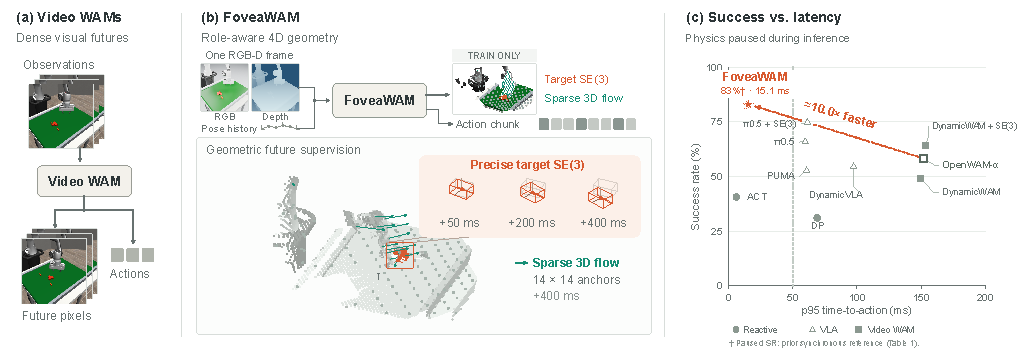
\includegraphics[width=\textwidth]{figures/Fig1/fig1.pdf}
\captionof{figure}{\textbf{\ours 按任务角色分配预测精度。}(a) 由真机 RGB 照片经 MoGe-2~\cite{moge2} 重建场景，叠加示意性的目标未来 SE(3) 位姿与稀疏 3D 流。(b) 表~\ref{tab:main} 中的 Native SR 与原生 p95 出动作时间。}
\label{fig:teaser}
\end{center}

% 图 1：跨栏首图（规格 2026-11-02）
\section{引言}
\label{sec:introduction}

从传送带上抓取零件、把物体放入移动的容器、接住从斜坡滚下的小球，都要求指令与其生效时刻的场景相符。从图像采集到夹爪闭合，策略需要推理，指令需要排队，机械臂也需要运动。传送带上以 0.10\,m/s 运动的零件在 150\,ms 延迟内会移动 15\,mm，超过平行夹爪抓取它所能容忍的 \fillin{X}\,mm。从扩散策略到视觉—语言—动作（VLA）模型与世界—动作模型（WAM）\cite{diffusionpolicy,pi05,dreamzero,openwam_alpha}，多数先进的视觉运动策略是在准静态场景中发展起来的，延迟在这些场景中影响很小 \cite{akinola2021dynamic,domino,dynamicvla}。

近期工作以三种方式加入时间上下文：以堆叠帧、光流或压缩视频 token 作为历史输入 \cite{tracevla,hifvla,pactwam,dynamicvla,dynamicwam}；用世界模型预测未来视频、隐变量、物体状态或速度场 \cite{dreamzero,dreamvla,domino,ahead}；以及在推理存在延迟时保持指令及时性的执行方案 \cite{rtc,vlash,chronos}。动态策略需要哪些信息、需要多高精度、针对哪个时刻，仍不清楚。我们认为，答案可以从交互误差的来源中寻找。抓取或放置的误差由指令生效时刻目标的度量位姿决定，场景其余部分则仅通过其留下的间隙起作用。像素历史隐含了这种运动，而图像空间的预测将大部分容量用于外观。

我们用物理时间中的误差预算具体说明这一观点（第~\ref{sec:formulation}~节）。它把接触误差分为定位、运动、时间、未建模动力学与旋转几项；场景其余部分则只在预测误差超过间隙时产生影响。这一代数推导很初等，延迟补偿在控制与跟踪中也已有长期研究 \cite{smith1957,azuma1994,barshalom2001}，但对学习型策略而言，误差预算提供了在场景中分配精度的方法，并给出可检验的预测，例如忽略运动的策略必然失败的领先时长界限。它也导出三项设计选择：\emph{记住}目标的度量运动，\emph{预测}目标的 SE(3) 轨迹及精度不超过间隙所需的环境 3D 流，并依据按生效时刻索引的预测与指令\emph{行动}。

我们围绕这些选择构建 \ours（图~\ref{fig:architecture}）。Transformer 编码当前 RGB-D 帧、机器人状态，以及因果位姿跟踪器给出的目标 SE(3) 历史。世界流在物理时域上预测目标的 SE(3) 轨迹与\QtwoSel{粗粒度}{粗粒度}{} 3D 场景流，动作流则生成以领先时长为条件的指令；领先时长是从图像采集到指令生效的时间。
\QthreeSel{动作 token 在每层读取世界流。}{动作流读取解码后的预测。}{世界流在训练时监督共享表示，部署时只运行动作流。}
对于真机，我们用现成的感知方法 \cite{pointworld,wilddet3d,sam2} 把 DROID \cite{droid} 提升为度量 4D 标签，并据此预训练基座模型。

我们在 \bench、DOMINO \cite{domino}、LIBERO \cite{libero} 和真实传送带上评测。\bench 包含我们构建的十四项仿真任务，能够分别改变误差预算中的各项；实时协议保证每种方法计算期间场景持续运动。\ours 在 \bench 留出场景上的成功率为 \fillin{XX.X}\%，比最强基线高 \fillin{X.X} 个百分点；不过，推理时暂停物理仿真后，一个更大的模型领先。SE(3) 历史在超过临界领先时长后带来帮助，而 RGB、光流或视频隐变量历史的增益很小。
\Qthree{1}{读取预测的收益随延迟增大，对静止目标则没有收益，这与测试时想象并无必要的报告 \cite{fastwam} 相协调。}%
\Qthree{2}{根据解码后的预测生成动作，其收益随延迟增大，对静止目标则没有收益，这与测试时想象并无必要的报告 \cite{fastwam} 相协调。}%
\Qthree{3}{只要在指令生效时刻监督预测，部署时去掉预测仍能保留大部分收益，与文献 \cite{fastwam} 在静态场景中的发现类似。}
误差预算的预测近似成立，偏差最大的是捕获任务\fillin{，且有一项任务仍未被任何方法解决}。我们的贡献包括：
\begin{itemize}[leftmargin=*,topsep=2pt,itemsep=1pt]
\item 一个物理时间中的简单误差预算，用于指导设计，并由实验检验其预测；
\item \ours：联合学习以领先时长为条件的动作与按角色区分的 4D 预测，以及在带有提升后 4D 标签的 DROID 上预训练的真机基座；
\item 采用实时协议的 \bench，\ours 在其上优于已有方法。我们将一并发布该基准、DROID 标签和代码。
\end{itemize}

\section{相关工作}
\label{sec:related_work}

\paragraph{动态操作。}补偿感知与执行之间的时间差是一个经典问题，从带纯滞后的控制 \cite{smith1957}，到用卡尔曼类滤波器跟踪目标并规划拦截的抓取系统 \cite{barshalom2001,allen1993,baeuml2010,marturi2019dynamic}；这些系统精确，但针对每种物体和任务专门设计。近来，学习型策略开始进入运动场景 \cite{dynamicvla}。PUMA 读取历史光流，并以未来物体特征作为监督 \cite{domino}；DynamicWAM 以光流和运动学描述子为 WAM 提供条件，并以实时分块方式执行 \cite{dynamicwam}。两者都从图像空间线索中推断过去的运动，而 \ours 以目标的度量 SE(3) 位姿历史为输入，只观测当前一帧 RGB-D。另一些动态策略预测显著 token \cite{ahead}、未来图像 \cite{dbctfp}、紧凑的未来编码 \cite{foretime} 或 3D 场景动力学 \cite{physmani}，并在测试时以这些预测为条件生成动作。DynaWM 针对动态操作调整基础 VLA 的动作块 \cite{dynawm}，DynamicManip 从单条静态示范合成动态示范 \cite{dynamicmanip}。执行调度方案通过让推理与执行重叠 \cite{dynamicvla,smolvla}、保持相邻动作块一致 \cite{rtc,bid}，或以执行时刻为条件 \cite{vlash}，来减小或掩盖延迟。它们决定的是动作何时计算、何时执行，而不是策略表示什么。DOMINO \cite{domino} 与 PhysMani-Bench \cite{physmani} 提供了多样的动态操作任务，但它们公开的默认评测流程只在策略返回预测之后才推进仿真。\bench 则在推理期间推进场景，并让每个方法承担其实测延迟。

\paragraph{WAM 中的预测监督。}世界—动作模型（WAM）在同一个网络中生成未来视频与动作 \cite{uwm,uva,dreamzero,openwam_alpha}，其基础是把视频预测作为策略目标 \cite{gr1,seer}。由于生成视频代价高，近期工作改变了预测的内容，例如动态区域、深度与语义特征 \cite{dreamvla}，与 RGB 并列的光流和几何 \cite{dreamwam}，物体掩码或物体槽 \cite{maskwam,oawam}，以及紧凑隐变量 \cite{flare,wog}；它们也在追问测试时是否需要预测。Fast-WAM 在不做测试时想象的情况下保留了视频建模的大部分收益 \cite{fastwam}，PUMA 与 SG-WAM 则在训练后去掉预测器 \cite{domino,sgwam}。\ours 沿用这种只在训练中使用预测的方式，但主要预测的是度量 4D 状态，而不是像素、特征或隐变量，因此目标未来的位姿得到显式监督，而不是停留在隐式。

\paragraph{以物体为中心与基于几何的运动表示。}度量 3D 输入使策略更精确、样本效率更高 \cite{peract,dp3}。运动已被表示为 2D 点轨迹 \cite{atm,track2act,im2flow2act}、3D 流 \cite{generalflow,flowdreamer,pointworld,physmani}，以及物体关键点或 SE(3) 轨迹 \cite{kpam,spot,objectforesight}；刚体分解也早已用于学习场景动力学 \cite{se3nets,se3posenets}。这些工作用同一种表示描述场景：要么处处是稠密的流或轨迹，要么每个物体一个位姿。以目标为中心的预测器（包括预测物体层面未来的动态 VLA）只建模目标的未来 \cite{domino,spot}，把阻挡或推动目标的物体排除在外。DOCIR 把机器人、目标与障碍物分开，但只把这种区分用作输入编码 \cite{docir}。\ours 按角色分配精度：粗粒度的稀疏 3D 流描述整个场景，接触依赖毫米级精度的目标另由其 SE(3) 历史与预测描述。

\section{\ours}
\label{sec:method}

\begin{figure*}[t]
\centering
\resizebox{\textwidth}{!}{% Fig. 2: architecture of the method (schematic in TikZ, v4 2026-10-23). Spec: docs/writing/v2_figure_specs.md (Fig. 2).
% Semantic colors: obscol (observation), predcol (prediction / world), actcol (action), gtcol (neutral).
% The picture is about 17.4 cm wide and is scaled to \textwidth, so \scriptsize prints at about 7 pt.
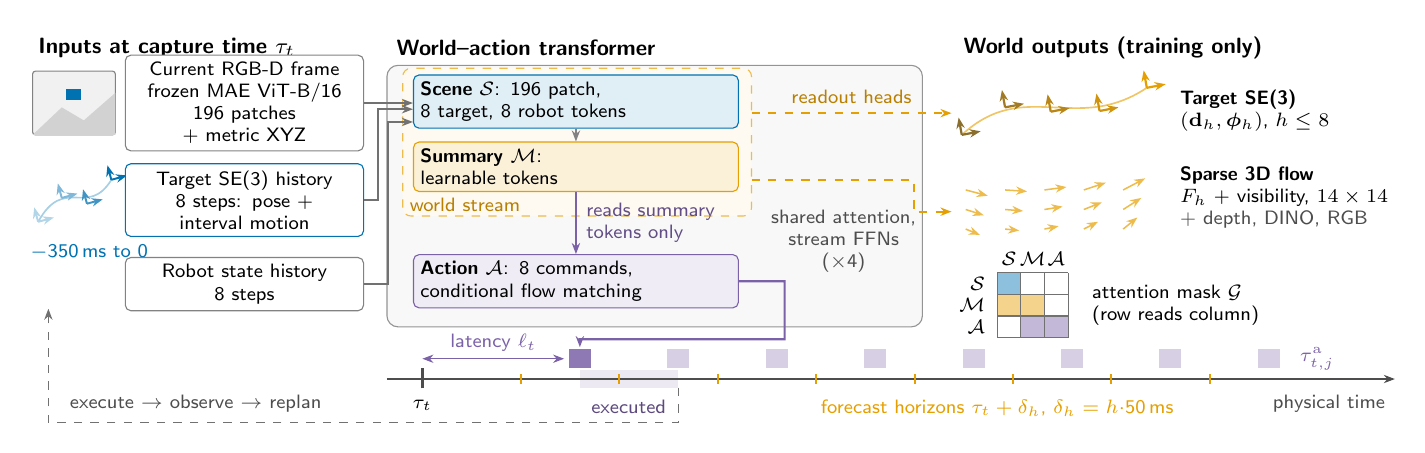
\begin{tikzpicture}[
  yscale=0.92,
  font=\sffamily\scriptsize,
  >={Stealth[length=4pt,width=3pt]},
  box/.style={draw=gtcol!70, rounded corners=2pt, align=center, inner sep=2.5pt, fill=white, text width=2.85cm},
  lane/.style={rounded corners=2pt, align=left, inner sep=2.5pt, minimum height=0.60cm, text width=3.95cm},
  flowarrow/.style={->, thick, gtcol!80},
  readout/.style={->, thick, predcol, dashed},
]
% ======================= Titles =======================
\node[font=\sffamily\footnotesize\bfseries, anchor=west] at (0,5.12) {Inputs at capture time $\tau_t$};
\node[font=\sffamily\footnotesize\bfseries, anchor=west] at (4.55,5.12) {World--action transformer};
\node[font=\sffamily\footnotesize\bfseries, anchor=west] at (11.75,5.12) {World outputs (training only)};
% ======================= Inputs =======================
\draw[gtcol!70, fill=gtcol!8, rounded corners=1pt] (0.05,3.92) rectangle (1.10,4.80);
\fill[gtcol!25] (0.05,3.92) -- (0.42,4.30) -- (0.70,4.12) -- (1.10,4.50) -- (1.10,3.92) -- cycle;
\fill[obscol] (0.48,4.40) rectangle (0.66,4.56);
\node[box, anchor=west] (img) at (1.22,4.36) {Current RGB-D frame\\frozen \cfgVisualEncoder\\\cfgPatches{} patches + metric XYZ};
\draw[obscol!35, line width=0.6pt] (0.12,2.72) .. controls (0.45,3.37) and (0.75,2.77) .. (1.05,3.30);
\foreach \x/\y/\o in {0.12/2.72/30, 0.42/3.05/50, 0.74/2.97/75, 1.05/3.30/100}{
  \begin{scope}[shift={(\x,\y)}]
    \draw[obscol!\o, line width=0.7pt, ->] (0,0) -- (0.20,0.06);
    \draw[obscol!\o, line width=0.7pt, ->] (0,0) -- (-0.05,0.20);
  \end{scope}}
\node[anchor=north west, text=obscol, inner sep=1pt] at (-0.02,2.45) {$-$\cfgHistorySpan{} to 0};
\node[box, anchor=west, draw=obscol] (hist) at (1.22,3.02) {Target SE(3) history\\\cfgHistoryLen{} steps: pose +\\interval motion};
\node[box, anchor=west] (robot) at (1.22,1.86) {Robot state history\\\cfgHistoryLen{} steps};
% ======================= Transformer =======================
\draw[gtcol!60, rounded corners=4pt, fill=gtcol!4] (4.55,1.27) rectangle (11.35,4.88);
\draw[predcol!70, rounded corners=3pt, fill=predcol!5, dashed] (4.75,2.80) rectangle (9.18,4.84);
\node[anchor=south west, text=predcol!80!black, inner sep=1pt] at (4.80,2.82) {world stream};
\node[lane, fill=obscol!12, draw=obscol] (laneS) at (6.95,4.38) {\textbf{Scene} $\mathcal S$: \cfgPatches{} patch,\\\cfgHistoryLen{} target, \cfgHistoryLen{} robot tokens};
\node[lane, fill=predcol!15, draw=predcol] (laneM) at (6.95,3.48) {\textbf{Summary} $\mathcal M$: \cfgMetaTokens{}\\learnable tokens};
\node[lane, fill=actcol!12, draw=actcol] (laneA) at (6.95,1.90) {\textbf{Action} $\mathcal A$: \cfgChunk{} commands,\\conditional flow matching};
\node[align=center, text=gtcol, text width=2.05cm] at (10.35,2.45) {shared attention,\\stream FFNs\\($\times$\cfgLayers)};
\draw[->, thick, gtcol!70] (laneS.south) -- (laneM.north);
\draw[->, thick, actcol] (laneM.south) -- node[right, text=actcol!80!black, align=left] {reads summary\\tokens only} (laneA.north);
% input arrows
\draw[flowarrow] (img.east) -- (laneS.west |- img.east);
\draw[flowarrow] (hist.east) -- ++(0.18,0) |- ([yshift=-3pt]laneS.west);
\draw[flowarrow] (robot.east) -- ++(0.30,0) |- ([yshift=-8pt]laneS.west);
% ======================= Outputs =======================
\draw[predcol!60, line width=0.6pt] (11.85,3.92) .. controls (12.65,4.72) and (13.30,3.92) .. (14.20,4.57);
\foreach \x/\y/\o in {11.85/3.92/40, 12.40/4.30/55, 12.98/4.24/70, 13.60/4.25/85, 14.20/4.57/100}{
  \begin{scope}[shift={(\x,\y)}]
    \draw[predcol!\o!gtcol, line width=0.8pt, ->] (0,0) -- (0.24,0.05);
    \draw[predcol!\o!gtcol, line width=0.8pt, ->] (0,0) -- (-0.04,0.24);
  \end{scope}}
\node[anchor=west, align=left] at (14.50,4.26) {\textbf{Target SE(3)}\\$(\vect d_h,\boldsymbol\phi_h)$, $h\le\cfgHorizons$};
\foreach \i in {0,...,4}{\foreach \j in {0,...,2}{
  \pgfmathsetmacro{\dx}{0.18+0.05*\j}
  \draw[predcol!70, ->, line width=0.55pt] ({11.90+0.50*\i},{2.62+0.27*\j}) -- ++(\dx,{0.06*\i-0.08});}}
\node[anchor=west, align=left] at (14.50,3.05) {\textbf{Sparse 3D flow}\\$F_h$ + visibility, \cfgContextGrid\\\textcolor{gtcol}{+ depth, DINO, RGB}};
\draw[readout] (9.18,4.22) -- (11.72,4.22);
\draw[readout] (9.18,3.30) -- (11.24,3.30) |- (11.72,2.86);
\node[anchor=south, text=predcol!80!black] at (10.45,4.22) {readout heads};
% attention mask (rows read columns): S, M, A
\def\mx{12.30}\def\my{1.12}\def\cs{0.30}
\foreach \r/\rn in {0/S,1/M,2/A}{
  \node[anchor=east] at (\mx-0.03,{\my+(2-\r)*\cs+0.5*\cs}) {$\mathcal{\rn}$};
  \node[anchor=south] at ({\mx+\r*\cs+0.5*\cs},{\my+3*\cs-0.04}) {$\mathcal{\rn}$};}
\foreach \r/\c/\col in {0/0/obscol, 1/0/predcol, 1/1/predcol, 2/1/actcol, 2/2/actcol}{
  \fill[\col!45] ({\mx+\c*\cs},{\my+(2-\r)*\cs}) rectangle ++(\cs,\cs);}
\draw[gtcol!80, shift={(\mx,\my)}] (0,0) grid[step=\cs] ({3*\cs},{3*\cs});
\node[anchor=west, align=left] at ({\mx+3*\cs+0.18},{\my+1.5*\cs}) {attention mask $\mathcal G$\\(row reads column)};
% ======================= Physical time =======================
% 1.25 cm per 50 ms; capture at x = 5.00, first execution at x = 7.00 (latency 80 ms in this sketch).
\fill[actcol!14] (7.00,0.43) rectangle (8.25,0.67);
\draw[->, gtcol] (4.55,0.55) -- (17.35,0.55);
\node[anchor=north east, text=gtcol] at (17.35,0.47) {physical time};
\draw[gtcol, line width=0.8pt] (5.00,0.42) -- (5.00,0.70);
\node[anchor=north] at (5.00,0.40) {$\tau_t$};
\foreach \h in {1,...,8}{\draw[predcol, line width=0.7pt] ({5.0+1.25*\h},0.48) -- ({5.0+1.25*\h},0.62);}
\node[anchor=north, text=actcol!75!black] at (7.62,0.40) {executed};
\node[anchor=north, text=predcol] at (12.30,0.40) {forecast horizons $\tau_t+\delta_h$, $\delta_h=h\cdot$\cfgHorizonStep};
\foreach \k in {0,...,7}{
  \pgfmathtruncatemacro{\shade}{\k<1 ? 85 : 30}
  \fill[actcol!\shade] ({6.86+1.25*\k},0.70) rectangle ++(0.28,0.26);}
\draw[<->, actcol] (5.00,0.83) -- (6.80,0.83) node[midway, above=-1pt] {latency $\ell_t$};
\node[anchor=west, text=actcol] at (16.02,0.83) {$\tapp_{t,j}$};
\draw[flowarrow, actcol] (laneA.east) -- (9.60,1.90) -- (9.60,1.10) -| (7.00,0.99);
% replan loop
\draw[->, dashed, gtcol!80] (8.25,0.43) -- (8.25,-0.05) -- (0.25,-0.05) -- (0.25,1.52);
\node[anchor=south west, text=gtcol] at (0.40,-0.04) {execute $\to$ observe $\to$ replan};
\end{tikzpicture}
}
\caption{\textbf{\ours。}条件 token $\mathcal Z$ 编码当前 RGB-D 帧、因果跟踪器给出的目标 SE(3) 历史以及机器人状态。物体查询 $\mathcal Q$ 与场景查询 $\mathcal F$ 在物理时域 $\tau_t+\delta_h$ 上回归目标的 SE(3) 轨迹以及带可见性的\QtwoSel{粗粒度}{粗粒度}{\cfgContextPoints{} 个点的} 3D 场景流，外观读出头提供额外的训练目标。动作 token $\mathcal A$ 生成以领先时长为条件、在 $\tapp_{t,j}$ 生效的指令，每 \cfgReplan{} 重规划一次。掩码 $\mathcal G$ 规定每个组读取哪些组。
\QthreeSel{动作 token 在每一层读取世界查询。}{动作 token 读取解码出的世界几何。}{动作 token 不读取任何世界 token，因此部署时只运行动作分支。}}
\label{fig:architecture}
\end{figure*}

\ours（图~\ref{fig:architecture}）是一个包含三组 token 的 Transformer：条件 token 编码当前观测与目标的运动历史，世界查询在物理时域上预测场景，动作 token 生成以领先时长为条件的指令。我们以确定性方式预测世界，用流匹配生成动作 \cite{flowmatching}。下面先说明促成这一设计的问题设定。

\subsection{在物理时间中行动}
\label{sec:formulation}

\paragraph{生效时刻。}
我们考虑一个连同采集时刻一起接收图像与机器人状态的策略。在查询 $t$，其历史为 $\mathcal H_t=\{(o_i,s_i,\tau_i)\}_{\tau_i\le\tau_t}$，输出一个动作块 $A_t=(\vect a_{t,0},\ldots,\vect a_{t,H-1})$，其中第 $j$ 条指令在
\begin{equation}
\tapp_{t,j}=\tau_t+\ell_t+j\Delta_a
\label{eq:apptime}
\end{equation}
生效，$\ell_t$ 是从采集到首次生效的延迟（预处理、推理、排队与执行），$\Delta_a$ 是控制周期。我们把 $\Delta_{t,j}=\tapp_{t,j}-\tau_t$ 称为指令 $j$ 的\emph{领先时长}；这条指令必须与 $\tapp_{t,j}$ 而不是 $\tau_t$ 时的场景相符（图~\ref{fig:principles}）。

\begin{figure}[t]
\centering
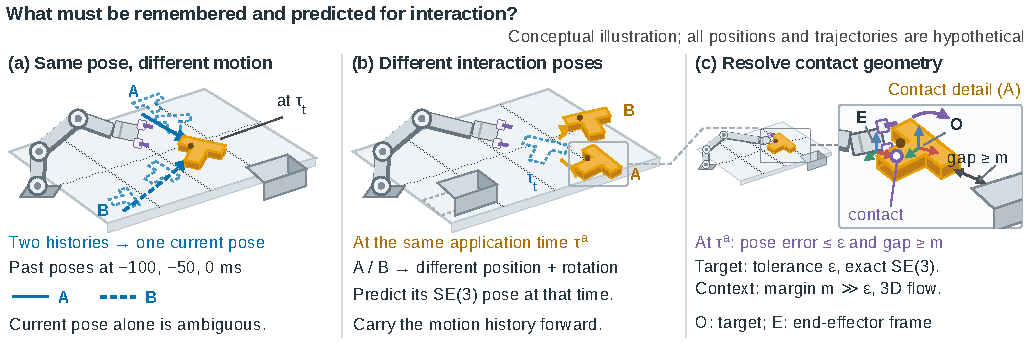
\includegraphics[width=\columnwidth,trim=0 0 0 26,clip]{interaction_timing.pdf}
\caption{\textbf{在物理时间中行动}（示意）。(a) 两段历史在采集时刻 $\tau_t$ 到达同一位姿，却意味着不同的运动。(b) 在生效时刻 $\tapp$，它们导致不同的目标位姿。(c) 接触要求末端坐标系 $E$ 与目标 $O$ 在 $\varepsilon$ 内对齐，而环境只通过它留下的间隙起作用，$m\gg\varepsilon$。}
\label{fig:principles}
\end{figure}

\paragraph{目标与环境。}
令 $W_t(\vect x,\tau)\in\R^3$ 为位于 $\vect x$ 的场景点在 $\tau_t$ 与 $\tau$ 之间的位移，在机器人基座坐标系中表示。\emph{目标} $\mathcal O$ 是其位姿误差进入接触或容纳容差 $\varepsilon$ 的刚体，例如要抓取的物体或要放入的料箱。\emph{环境} $\mathcal C$ 包含只需以间隙 $m$ 避开的物体——传送带或遮挡物。同一物体可以同时扮演两种角色，例如入口必须精确对准、环路必须避开的导线。在目标上，运动场由其位姿 $T(\tau)=(R(\tau),\vect p(\tau))\in\mathrm{SE}(3)$ 决定：
\begin{equation}
W_t(\vect x,\tau)=T(\tau)\,T(\tau_t)^{-1}\vect x-\vect x,\qquad \vect x\in\mathcal O .
\label{eq:rigidfield}
\end{equation}

\paragraph{误差从何而来。}
设策略显式或隐式地依据目标在 $\tapp$ 时位姿的估计 $\hat T$ 行动。对力臂为 $r$ 的接触点与旋转误差 $\theta$，接触误差至多为 $\|\hat{\vect p}(\tapp)-\vect p(\tapp)\|+2r\sin(\theta/2)$。把领先时长 $\Delta$ 内的运动写成匀速 $\vect v$ 加残差 $\boldsymbol\rho$（加速度、滚动、撞击），得到
\begin{equation}
\|\hat{\vect p}(\tapp)-\vect p(\tapp)\|\le
e_{\rm loc}+\hat\Delta\,e_{v}+\|\vect v\|\,e_{\tau}+e_{\rm dyn},
\label{eq:budget}
\end{equation}
四项依次为当前位置误差、速度误差乘领先时长、时间误差乘速度，以及残差运动的误差（附录~\appref{app:analysis}）。对于环境，只有当沿指令路径某处的预测误差至少为 $m$ 时才会发生碰撞。因此，忽略运动的策略一旦 $\|\vect v\|\Delta$ 超过 $\varepsilon$ 就会失手，而环境可以预测得粗得多。这些观察促成了 \ours 的三个部分，当前位置（$e_{\rm loc}$）则依赖位姿跟踪器：度量的运动历史，针对速度误差 $e_v$（第~\ref{sec:remember}~节）；目标的 SE(3) 预测加粗粒度环境流，针对 $e_{\rm dyn}$ 与旋转误差（第~\ref{sec:predict}~节）；知道自身领先时长、并与生效时刻的预测一起训练的指令，针对 $e_\tau$（第~\ref{sec:act}~节）。

\subsection{度量的目标运动历史}
\label{sec:remember}
我们用因果跟踪器在每个全分辨率 RGB-D 帧中估计目标位姿。SAM~2 从目标上的提示出发传播掩码 \cite{sam2}，FoundationPose 依据 CAD 模型或少量参考视图跟踪物体 \cite{foundationpose}。两者都没有时，我们使用逐帧估计度量包围盒位姿的单目三维检测器 \cite{wilddet3d}。每个估计只输出一次，带有其采集时刻与有效标志，之后的帧不会修改它。我们在 $-350,-300,\ldots,0$\,ms 处对这条因果轨迹重采样，使其含义不依赖于相机频率，并构建 \cfgHistoryLen{} 个运动 token，包含区间运动、有限差分速度与加速度以及当前位姿，均在基座坐标系与物理单位下表示（附录~\appref{app:tokens}）。冻结的 \cfgVisualEncoder{} \cite{mae} 把当前 RGB 图像编码为 \cfgPatches{} 个图像块 token，深度图为每个图像块提供用于旋转位置注意力的度量 3D 位置。机器人 token 保存 \cfgHistoryLen{} 个末端状态以及为第一个生效时刻指令的位姿。模型不接收过去的图像；训练时它使用与测试时相同的因果位姿估计，包括跟踪失败。

\subsection{按角色划分的 4D 预测}
\label{sec:predict}
世界查询在时域 $\tau_t+\delta_h$ 上预测 $W_t$，其中 $\delta_h=h\cdot$\cfgHorizonStep{}，$h=1,\ldots,\cfgHorizons$，覆盖下一次重规划之前所执行指令的领先时长，使预测在指令生效的时刻受到监督（附录~\appref{app:budget_leads}）。目标通过式~\eqref{eq:rigidfield} 参数化。对每个时域，
\begin{equation}
\vect d_h=\vect p(\tau_t{+}\delta_h)-\vect p(\tau_t),\;\;
\boldsymbol\phi_h=\Log\!\big(R(\tau_t{+}\delta_h)R(\tau_t)^{\!\top}\big)^{\vee}.
\label{eq:poselabel}
\end{equation}
物体查询以平方平移误差加 $\lambda_R$ 倍平方测地旋转误差回归 $(\vect d_h,\boldsymbol\phi_h)$（$\mathcal L_P$）。对旋转对称的目标，我们排除绕对称轴的不可观测旋转。场景的其余部分表示为 3D 场景流，即固定 \cfgContextGrid{} 图像网格上 $N=\cfgContextPoints$ 个点在基座坐标系中的位移 $F_h\in\R^{N\times3}$，这些点在工作空间中相距约 \fillin{X}\,mm。每个点对应一个带角色嵌入（目标、机器人或环境）的场景查询，回归该点的位移与可见性（$\mathcal L_F$）。\QtwoSel{网格刻意取得较粗，因为环境的误差在其间隙之内都可以容忍。}{网格刻意取得较粗，因为环境的误差在其间隙之内都可以容忍。}{其分辨率是在我们基准中最窄间隙处仍能保持成功率的最粗网格。}未来深度、DINOv3 特征 \cite{dinov3} 与运动表面的 RGB 作为场景查询的额外训练目标（$\mathcal L_{\rm aux}$）。所有标签都从当前状态累计，损失只使用有效标签。

\subsection{以领先时长为条件的动作}
\label{sec:act}
一个动作块包含 \cfgChunk{} 条按式~\eqref{eq:apptime} 的时刻生效的指令，控制周期 $\Delta_a$ 为 50\,ms（\cfgControlRate{}）。每 \cfgReplan{} 重规划一次时，动作块的前两条指令会在下一个动作块替换其余指令之前执行。每条指令是末端在基座坐标系中的平移与左乘相对旋转，外加一个夹爪指令，以为前一个生效时刻所指令的位姿为参考，这一位姿控制器确切知道 \cite{vlash}。每个动作 token 嵌入其领先时长 $\Delta_{t,j}=\ell_t+j\Delta_a$。训练时我们采样 $\ell\sim\mathcal U[0,\cfgLatencyMax]$，并从示范的 $\tau_t+\ell+j\Delta_a$ 处读取指令标签，因此一个模型可服务于该范围内的任何延迟。对归一化的动作块 $\vect a_1$、噪声 $\vect a_0\sim\mathcal N(0,I)$ 与 $u\sim\mathcal U[0,1]$，动作损失为
\begin{equation}
\mathcal L_A=\mathbb E\,\big\|v_\psi(\vect a_u,u\mid\mathcal Z_t,\hat{\mathcal W}_t,\mathcal G)-(\vect a_1-\vect a_0)\big\|^2,
\label{eq:fm}
\end{equation}
其中 $\vect a_u=(1-u)\vect a_0+u\vect a_1$，$\mathcal Z_t$ 为条件 token，$\hat{\mathcal W}_t$ 为耦合方式允许动作读取的世界 token（R0 与 R1 中没有）。总损失为 $\mathcal L=\mathcal L_A+\lambda_F\mathcal L_F+\lambda_P\mathcal L_P+\lambda_{\rm aux}\mathcal L_{\rm aux}$。

\paragraph{世界—动作耦合。}
注意力掩码 $\mathcal G$ 作用于四个 token 组：条件 $\mathcal Z$、物体查询 $\mathcal Q$、场景查询 $\mathcal F$ 与动作 $\mathcal A$。条件 token 只相互读取；世界查询读取条件与彼此；动作 token 读取条件、自身以及耦合方式所允许的那部分世界。
\Qthree{1}{动作 token 在每一层读取 $\mathcal Q$ 与 $\mathcal F$ 的隐藏状态，而世界不读取动作。}%
\Qthree{2}{我们每次查询预测一次世界，把解码出的目标轨迹与场景流编码为几何条件 token，并由它们以 \cfgEuler{} 步欧拉积分生成动作。训练时梯度穿过预测的几何反向传播，不使用教师强制。}%
\Qthree{3}{动作不读取任何世界 token。世界损失在训练中塑造共享参数，部署时只运行动作分支。}
\Bbone{1}{两个分支共享注意力投影，各自拥有前馈网络。}%
\Bbone{2}{世界分支与动作分支参数分离，条件 token 经过世界组，因此世界监督也塑造动作所读取的内容。}
第~\ref{sec:principles}~节把这一选择与其他方案进行比较，记号如下：R0 关闭世界损失，R1 中动作不读取任何世界 token，R2 中动作读取世界查询的隐藏状态，R3 中世界读取带噪动作，R4 双向开放，R5 把解码出的几何编码后供动作读取（附录~\appref{app:coupling}）。

\paragraph{执行与实现。}
测试时，我们依据执行器的延迟估计设定领先时长，即近期推理时间的 p95 加执行延迟。Transformer 有 \cfgLayers{} 层、宽度 \cfgWidth{}、\cfgHeads{} 个头，主干参数 \cfgBackboneParams{}，可训练参数共 \cfgTrainableParams{}。图像编码器与 DINOv3 教师保持冻结，但在每个训练步都要运行，并占据了其主要开销。在 \bench 上，我们以数据并行训练 4 个 epoch（全局 batch 为 16 时约 40k 次更新），在 \cfgTrainHardwareZh{} 上每个训练种子约需 \cfgTrainHours{} 小时。测试时，动作分支以半精度进行 \cfgEuler{} 步欧拉积分，在一块 \cfgGPU{} 上的 p95 出动作时间为 \fillin{XX}\,ms（附录~\appref{app:recipe} 与附录~\appref{app:timing}）。

\subsection{在提升为 4D 的真实机器人数据上预训练}
\label{sec:pretraining}
真实机器人数据不提供物体位姿或场景流。我们不使用物体模型，将 DROID \cite{droid} 提升为度量 4D 标签。场景流来自 PointWorld 为 DROID 发布的 3D 轨迹与优化后的相机标定 \cite{pointworld}。我们把指令中提到的物体作为目标：开放词汇检测器找到它 \cite{groundingdino}，SAM~2 跟踪其掩码，单目三维检测器估计其度量位姿。输入来自前向跟踪，与部署时一致；式~\eqref{eq:poselabel} 的标签来自整段回合上平滑的前向—后向跟踪。DROID 中的目标大多在机器人移动它们时才运动（\fillin{X}\% 的窗口在接触前出现目标运动），因此预训练主要教会模型度量几何、3D 流以及它们与以领先时长为条件的动作之间的耦合（图~\appref{fig:lifting}）。真机策略从这一基座初始化。仿真模型从通用初始化（冻结的 MAE 编码器加随机初始化的 Transformer）训练，另有一组受控比较在 \bench 上对基座做后训练（附录~\appref{app:pretraining}）。

\section{实验}
\label{sec:experiments}
我们在仿真和真机上比较 \ours 与反应式、动态及世界—动作策略（第~\ref{sec:main_results}~节与第~\ref{sec:real}~节），然后对目标历史与未来监督做消融（第~\ref{sec:principles}~节）。

\subsection{设置}
\label{sec:setup}

\paragraph{\bench。}
我们在 MuJoCo/robosuite \cite{mujoco,robosuite} 中构建了五个任务族共 14 个任务：抓取运动目标（简谐、传送带、平移、旋转与遮挡运动）、放入移动的容器、让棒沿旋转的导线穿过、捕获滚动或滑动的物体，以及撞击后的抓取（附录~\appref{app:benchmark}，图~\appref{fig:benchmark_tasks}）。我们在原任务运动范围内扫描附加延迟（0--200\,ms）。使用仿真特权状态的专家为每个任务提供 \cfgDemos{} 条示范。我们在开发场景上选择配置，并在 1{,}400 个留出场景（每个任务 100 个，新种子）上报告 \bench 主要比较与最终模型消融。最终模型的消融取三个训练种子的平均；筛选研究的种子与划分分别见附录~\appref{app:design}。每个基线训练一次。我们给出对留出场景自助法得到的配对 95\% 区间。

\paragraph{协议。}
观测、场景运动与执行共用一个控制周期为 50\,ms 的物理时钟。所有方法在同一执行器下运行，方法计算期间物理世界按其在一块 \cfgGPU{} 上测得的延迟继续推进。一条指令执行完毕且上一次推理结束后，策略再次被查询；新动作块到达之前，执行器继续执行上一个动作块。+150\,ms 设置为每个方法额外加入 150\,ms 延迟，暂停设置在推理期间停止物理仿真（附录~\appref{app:sweeps}）。我们报告按任务等权的成功率（SR）、接触时刻误差 $e_t$、首次接触时的位置误差 $e_p$ 以及 p95 出动作时间。

\paragraph{基线。}
我们比较反应式策略（ACT \cite{act}、Diffusion Policy \cite{diffusionpolicy} 与 $\pi_{0.5}$ \cite{pi05}）、动态 VLA（DynamicVLA \cite{dynamicvla} 与 PUMA \cite{domino}）、图像或隐空间 WAM（DreamVLA \cite{dreamvla} 与 OpenWAM-$\alpha$ \cite{openwam_alpha}），以及一个动态 WAM（DynamicWAM \cite{dynamicwam}）。每个基线使用其官方代码、输入与训练配方，在相同示范上训练；若其配方使用腕部相机，则提供渲染的腕部图像（附录~\appref{app:evaluation}）。\ours 只使用主视角，但还使用深度和目标位姿。为了控制目标运动信息的可用性，$\pi_{0.5}$ 与 DynamicWAM 还额外接收我们的 SE(3) 历史 token（+SE(3)）；它们的深度输入仍与本文方法不同。\emph{匀速输入}对照是去掉预测损失、改为接收目标位姿匀速外推作为输入 token 的 \ours。

% Transcribed from results/realtime_c/ (INFER0): ACT/DP native/+150 ms/Paused SR and 5090 p95. Other results pending.
% Highlight reported values per column with \bestcell/\secondcell (SR: highest; p95: lowest); exclude pending cells.
\begin{table}[t]
\centering\footnotesize
\caption{\tablelang{\textbf{Main results.} Task-balanced SR on 1{,}400 held-out \bench scenes: native latency, +150\,ms, and paused physics. Three training seeds for \ours, one per baseline. p95: time-to-action on \cfgGPU{}. Wrist and history denote extra inputs (Sec.~\ref{sec:setup}). Blue/bold and light blue mark the best and second reported values per column; rankings remain provisional while results are pending.}{\textbf{主要结果。}1{,}400 个 \bench 留出场景的任务均衡 SR：原生延迟、+150\,ms 和暂停物理。\ours 训练三个种子，基线各一个。p95：\cfgGPU{} 上的出动作时间。腕部及历史列表示额外输入（第~\ref{sec:setup}~节）。每列已有结果的最佳值为粗体加蓝底，次佳为浅蓝底；结果待齐，排名为暂时性比较。}}
\label{tab:main}
\setlength{\tabcolsep}{0.8pt}
\begin{tabular}{@{}lccccrrrr@{}}
\toprule
 & & \multicolumn{3}{c}{\tablelang{History}{历史}} & \multicolumn{3}{c}{SR (\%) $\uparrow$} & \\
\cmidrule(lr){3-5}\cmidrule(lr){6-8}
\tablelang{Method}{方法} & \tablelang{Wrist}{腕部} & RGB & \tablelang{Flow}{光流} & SE(3) & \tablelang{Native}{原生} & \makecell{+150\\ms} & \tablelang{Paused}{暂停} & \makecell{p95\\(ms)\\$\downarrow$} \\
\midrule
ACT \cite{act} &  &  &  &  & \bestcell{42.0} & \bestcell{24.1} & \bestcell{40.9} & \bestcell{10.7} \\
DP \cite{diffusionpolicy} &  & \cmark &  &  & \secondcell{0.0} & \secondcell{0.0} & \secondcell{33.1} & \secondcell{1701.9} \\
$\pi_{0.5}$ \cite{pi05} &  &  &  &  & \resultplaceholder & \resultplaceholder & \resultplaceholder & \resultplaceholder \\
$\pi_{0.5}$+SE(3) & \resultplaceholder &  &  & \cmark & \resultplaceholder & \resultplaceholder & \resultplaceholder & \resultplaceholder \\
\midrule
DynamicVLA \cite{dynamicvla} &  & \cmark &  &  & \resultplaceholder & \resultplaceholder & \resultplaceholder & \resultplaceholder \\
PUMA \cite{domino} &  &  & \cmark &  & \resultplaceholder & \resultplaceholder & \resultplaceholder & \resultplaceholder \\
\midrule
DreamVLA \cite{dreamvla} &  & \cmark &  &  & \resultplaceholder & \resultplaceholder & \resultplaceholder & \resultplaceholder \\
OpenWAM-$\alpha$ \cite{openwam_alpha} &  &  &  &  & \resultplaceholder & \resultplaceholder & \resultplaceholder & \resultplaceholder \\
\midrule
DynamicWAM \cite{dynamicwam} &  &  & \cmark &  & \resultplaceholder & \resultplaceholder & \resultplaceholder & \resultplaceholder \\
DynamicWAM+SE(3) & \resultplaceholder &  & \cmark & \cmark & \resultplaceholder & \resultplaceholder & \resultplaceholder & \resultplaceholder \\
\midrule
\ours &  &  &  & \cmark & \resultplaceholder & \resultplaceholder & \resultplaceholder & \resultplaceholder \\
\bottomrule
\end{tabular}
\end{table}


\subsection{主要结果}
\label{sec:main_results}
\ours 在 \bench 留出场景上的 SR 为 \fillin{XX.X}\%（表~\ref{tab:main}），比最强基线 \fillin{最强基线名称} 高 \fillin{X.X} 个百分点，比接收相同 SE(3) 历史的最强基线 \fillin{名称} 高 \fillin{X.X} 个百分点。优势最大的是 \fillin{旋转目标以及快速的传送带和平移目标}，即领先时长内目标移动最远的任务。它的 p95 出动作时间为 \fillin{XX}\,ms，是图像空间 WAM 的 \fillin{X} 分之一；后者的延迟会叠加到它们需要弥补的领先时长上。加入 150\,ms 延迟后，\ours 保持 \fillin{XX.X}\%，而反应式策略降至 \fillin{XX.X}\%，图像空间 WAM 降至 \fillin{XX.X}\%。推理期间暂停物理仿真时，它与 \fillin{暂停设置下最强基线名称} 的差为 \fillin{$\pm$X.X} 个百分点，从而把速度的贡献与表示的贡献区分开。匀速输入变体落后 \ours \fillin{X.X} 个百分点。我们结合无未来监督对照解释这一差异；后者既没有预测损失，也没有外推输入 token。DOMINO \cite{domino} 上的结果见附录~\appref{app:external}。

\subsection{真机实验}
\label{sec:real}

% Planned results: six-task real-robot study; numeric results and baseline selection pending.
\begin{table}[t]
\centering\footnotesize
\caption{\tablelang{\textbf{Real-robot result template.} Six planned tasks: T1 conveyor grasping, T2 moving-receptacle placement, T3 turntable grasping, T4 moving-car grasping, T5 post-collision interception, and T6 ramp interception. Trial counts and baseline selection await confirmation. Cells reserve success rates (\%); All pools the trials.}{\textbf{真机结果模板。}六个计划任务：T1 传送带抓取、T2 移动容器放置、T3 转盘抓取、T4 移动小车抓取、T5 碰撞后拦截、T6 斜坡拦截。试验数与基线选择待确认。单元格预留成功率（\%）；All 合并全部试验。}}
\label{tab:real}
\setlength{\tabcolsep}{2pt}
\resizebox{\columnwidth}{!}{%
\begin{tabular}{@{}lccccccc@{}}
\toprule
\tablelang{Method}{方法} & T1 & T2 & T3 & T4 & T5 & T6 & All \\
\midrule
\fillin{$\pi_{0.5}$} & \resultplaceholder & \resultplaceholder & \resultplaceholder & \resultplaceholder & \resultplaceholder & \resultplaceholder & \resultplaceholder \\
\fillin{DynamicWAM} & \resultplaceholder & \resultplaceholder & \resultplaceholder & \resultplaceholder & \resultplaceholder & \resultplaceholder & \resultplaceholder \\
\tablelang{\ours, no DROID base}{\ours，无 DROID 基座} & \resultplaceholder & \resultplaceholder & \resultplaceholder & \resultplaceholder & \resultplaceholder & \resultplaceholder & \resultplaceholder \\
\ours & \resultplaceholder & \resultplaceholder & \resultplaceholder & \resultplaceholder & \resultplaceholder & \resultplaceholder & \resultplaceholder \\
\bottomrule
\end{tabular}}
\end{table}


我们在\cfgRobotZh{}上评估六个任务（图~\appref{fig:real_setup}，表~\appref{tab:real_tasks}），比较 \ours、$\pi_{0.5}$、DynamicWAM 与 Diffusion Policy \cite{diffusionpolicy}：传送带抓取（T1）、放入传送带上的容器（T2）、转盘抓取（T3）、抓取运动的玩具小车（T4）、拦截碰撞后的球（T5），以及拦截沿斜坡滚落或滑落的物体（T6）。它们涵盖直线、圆周、平面自由运动、撞击后运动与重力加速运动。每个方法在相同的 100 条遥操作示范上逐任务训练或微调，另用独立的 20 条示范验证，并以共享的试验键在每个任务上运行 20 次试验。\ours 用\fillin{跟踪器}跟踪目标，在一块 \cfgGPU{} 上运行，p95 出动作时间为 \fillin{XX}\,ms。它在全部试验中的成功率为 \fillin{XX.X}\%，\fillin{最强基线}为 \fillin{XX.X}\%（表~\ref{tab:real}）。\fillin{优势最大的任务及主要失败模式}（图~\ref{fig:real_trials}）。

\begin{figure}[t]
\centering
\figplaceholder[1.45in]{\columnwidth}{图 4——真机试验}{%
\textbf{行：}\ours 的一次成功；最强基线在同一试验键上的表现；\ours 的一次失败。
\textbf{列：}查询帧、首个执行时刻 $\tapp$ 与接触时刻。\textbf{叠加：}\textcolor{obscol}{蓝色}为跟踪得到的过去位姿；\textcolor{actcol}{紫色}为指令的夹爪路径。真实照片不做修饰；叠加来自各次试验的日志数据。}
\caption{\textbf{真机试验}：\ours 与\fillin{最强基线}在同一试验键上的表现（上两行），以及 \ours 的一次失败（下）。\fillin{对所选试验的一句话说明。}}
\label{fig:real_trials}
\end{figure}

\subsection{消融：动态策略需要什么？}
\label{sec:principles}
四个核心对照使用最终 24 层模型与配方，每个对照训练三个种子，数据与训练预算相同（表~\ref{tab:design}）。它们检验目标历史、未来监督、场景流监督和专用目标位姿监督。各对照在实时协议下评估 0 与 150\,ms 附加延迟，完整模型的参考结果复用第~\ref{sec:main_results}~节。更广泛的设计选择在 4 层模型上筛选，各组配方见附录~\appref{app:design}。

% Planned results: A4 final 24-layer confirmation, four controls x three training seeds, real-time C at added 0/150 ms. Full-model reference reused from A1; no screening numbers substituted.
\begin{table}[t]
\centering\footnotesize
\caption{\tablelang{\textbf{Core ablations} of the final 24-layer model on held-out \bench scenes (three training seeds). Each row changes one component of
\ours (\sel). Native, +150\,ms: success (\%) with native latency and with 150\,ms of added latency. Bottom: the CV-input alternative, which replaces the forecast losses by constant-velocity extrapolations as input tokens. $e_p$: position
error at first contact (mm). p95: time-to-action (ms).}{\textbf{核心消融}（最终 24 层模型，\bench 留出场景，三个训练种子）。每行只改变 \ours（\sel）的一个组件。
原生、+150\,ms：原生延迟下与附加 150\,ms 延迟下的成功率（\%）；下方为匀速外推输入的替代方案，它以匀速外推作为输入 token 取代预测损失；$e_p$：首次接触时的位置误差（mm）；p95：出动作时间（ms）。}}
\label{tab:design}
\setlength{\tabcolsep}{2.9pt}
\begin{tabular}{@{}lcccc@{}}
\toprule
\tablelang{Variant}{变体} & \tablelang{Native}{原生} & +150\,ms & $e_p$ & p95 \\
\midrule
\ours\sel & \resultplaceholder & \resultplaceholder & \resultplaceholder & \resultplaceholder \\
\tablelang{No target history}{无目标历史} & \resultplaceholder & \resultplaceholder & \resultplaceholder & \resultplaceholder \\
\tablelang{No future supervision}{无未来监督} & \resultplaceholder & \resultplaceholder & \resultplaceholder & \resultplaceholder \\
\tablelang{No scene-flow supervision}{无场景流监督} & \resultplaceholder & \resultplaceholder & \resultplaceholder & \resultplaceholder \\
\tablelang{No dedicated SE(3)}{无专用 SE(3)} & \resultplaceholder & \resultplaceholder & \resultplaceholder & \resultplaceholder \\
\midrule
\tablelang{CV input}{匀速外推输入} & \resultplaceholder & \resultplaceholder & \resultplaceholder & \resultplaceholder \\
\bottomrule
\end{tabular}
\end{table}


\begin{figure*}[t]
\centering
\figplaceholder[1.55in]{\textwidth}{图 5——消融（四个子图）}{%
\textbf{(a) 历史。}完整模型与无目标运动历史在 0 和 150\,ms 附加延迟下的 SR 差值。
\textbf{(b) 未来监督。}完整模型与关闭全部未来损失，按任务族分组。
\textbf{(c) 几何监督。}完整模型、无场景流和无专用 SE(3)，按任务族分组。
\textbf{(d) 成功率与延迟。}完整模型与四个对照在 0 和 150\,ms 附加延迟下的 p95 出动作时间与 SR。
各面板复用相同留出轨迹与三个训练种子，显示 95\% 配对自助法区间。}
\caption{\textbf{最终模型规模上的核心消融。}(a) 目标运动历史。(b) 未来监督。(c) 两项几何监督。(d) 实时协议下的成功率与延迟。\fillin{四个对照完成后概括实测效应。}}
\label{fig:analysis}
\end{figure*}

\paragraph{记住什么。}
无历史对照保留当前图像、当前目标位姿和八个机器人状态，移除过去的目标位姿及其速度、加速度特征。它相对完整模型的 SR 差值在 0\,ms 时为 \fillin{带符号 X.X} 个百分点，在 150\,ms 附加延迟时为 \fillin{带符号 X.X} 个百分点（图~\ref{fig:analysis}a）。视觉历史替代方案属于 4 层筛选，不是最终规模的对照。位姿噪声鲁棒性单独用冻结权重评测（附录~\appref{app:design_remember}）。

\paragraph{预测什么。}
无未来对照关闭 SE(3)、场景流及可见性、未来深度、DINO 与动态 RGB 损失，保留当前目标 RGB 重建，用于检验未来监督的整体作用（图~\ref{fig:analysis}b）。另外两个对照保留全部外观目标：一个只移除场景流与可见性监督，另一个只移除专用 SE(3) 监督。后者仍用同一 \cfgContextGrid{} 流覆盖目标、机器人与周围环境，场景各部分均使用相同的粗粒度表示。前者检验场景流监督的作用，不能单独归因于环境信息。两者的带符号 SR 差值在 0\,ms 时为 \fillin{X.X} 和 \fillin{X.X} 个百分点，在 150\,ms 时为 \fillin{X.X} 和 \fillin{X.X} 个百分点；图~\ref{fig:analysis}c 按任务族分解这些效应。

\begin{figure}[t]
\centering
\figplaceholder[1.35in]{\columnwidth}{图 6——执行时刻的预测}{%
\textbf{行：}一次滚动捕获（预测误差为中位数）与一次失败的撞击后抓取。\textbf{列：}$\tau_t$ 的查询帧、$\tapp$ 的帧，以及基座坐标系中的 3D 小图。
\textbf{叠加：}\textcolor{obscol}{蓝色}为过去位姿，\textcolor{predcol}{橙色}为训练期预测头给出的预测三轴与粗粒度流箭头，\textcolor{gtcol}{灰色}为同一时刻的真值，\textcolor{actcol}{紫色}为指令路径。完整示例见图~\appref{fig:qualitative}。}
\caption{\textbf{执行时刻的预测}（\bench 留出回合，读自训练期预测头）。上：SE(3) 预测跟随滚动目标，而外推冲过了头。下：撞击之前，回归得到的预测对可能的结果取平均，抓取落空。}
\label{fig:forecasts}
\end{figure}

\paragraph{如何使用预测。}
最终模型只把预测用于训练监督。4 层耦合研究的三个种子中，把预测送给动作没有带来稳定增益（附录~\appref{app:design_act}）；该结果不能证明最终规模下的等效性。最终模型开启未使用的预测头时，只检查固定输入与噪声下的动作一致性并测量额外代价。实时协议下，额外延迟可能改变闭环轨迹。图~\ref{fig:analysis}d 报告四个训练对照的实测成功率与延迟，不包含最终规模的 R5 比较。

\section{结论}
\label{sec:conclusion}

\ours 把精度花在接触所依赖之处：它精确建模目标的度量运动、粗略建模整个场景，并只用这些预测来训练它据以行动的表示。在 \bench、DOMINO 与六个真机任务上，它都优于反应式、动态与世界—动作策略。\fillin{消融表明，目标历史在附加延迟下作用最大，未来监督在不改变推理计算的情况下改善控制。}\fillin{说明专用 SE(3)、场景流与统一精度对照支持什么：更好的预测设计，或者在任务分组也一致时，按角色分配精度。}计入推理延迟后，\fillin{说明成功率与相对表现与暂停评测相比有何不同}。

\paragraph{局限性。}
\ours 需要一个指定的刚体目标及其可靠的位姿估计，其预测也不建模机器人自身的接触如何改变目标的运动。目标轨迹预测头在每个时域只预测一个未来，不表示不确定性或多模态运动；不确定性感知的预测可以弥补这一点。

\FloatBarrier
\clearpage
\section*{LLM Usage Statement（大语言模型使用声明）}
\label{sec:llm_usage}
我们使用 OpenAI Codex 辅助文献调研、代码实现与调试、实验执行及论文语言润色。
Codex 还用于辅助编写绘图代码，以及调整图表与论文排版。
作者审阅了 AI 辅助生成或修改的内容，对照原始来源核查了参考文献，并通过测试与实验验证了实现。
作者对最终稿件、实验结果和结论承担全部责任。

\bibliographystyle{ieeenat_fullname}
\begingroup
\small
\setlength{\bibsep}{2pt}
\bibliography{references}
\endgroup
\clearpage
\appendix
\setcounter{table}{0}
\setcounter{figure}{0}
\setcounter{equation}{0}
\renewcommand{\thetable}{S\arabic{table}}
\renewcommand{\thefigure}{S\arabic{figure}}
\renewcommand{\theequation}{S\arabic{equation}}
\renewcommand{\theHtable}{supp.\arabic{table}}
\renewcommand{\theHfigure}{supp.\arabic{figure}}
\renewcommand{\theHequation}{supp.\arabic{equation}}
% 中文附录装配，与英文 appendix/content.tex 一一对应。
\section{延迟下行动的误差分析}
\label{app:analysis}

本附录推导第~\mainref{sec:formulation}~节的误差分解，把它推广到旋转、环境与分块执行，推导简单的比例关系，给出 \bench 中各项的量级，并说明其不适用的情形。这一分解促成了 \ours 的设计，它不是成功率的模型。

\subsection{平移}
\label{app:budget_translation}
设执行时刻目标的真实位置为 $\vect p(\tapp)=\vect p(\tau_t)+\vect v\Delta+\boldsymbol\rho$，策略的估计为 $\hat{\vect p}(\tapp)=\hat{\vect p}(\tau_t)+\hat{\vect v}\hat\Delta+\hat{\boldsymbol\rho}$。减去再加上 $\vect v\hat\Delta$ 得到恒等式
\begin{equation}
\begin{aligned}
\hat{\vect p}(\tapp)-\vect p(\tapp)
={}&\big[\hat{\vect p}(\tau_t)-\vect p(\tau_t)\big]+(\hat{\vect v}-\vect v)\hat\Delta\\
&+\vect v(\hat\Delta-\Delta)+(\hat{\boldsymbol\rho}-\boldsymbol\rho),
\end{aligned}
\label{eq:budget_identity}
\end{equation}
由三角不等式即得式~\mainref{eq:budget}。由于 $\vect v$ 是 $\tau_t$ 时的速度，$\boldsymbol\rho$ 恰好是匀速外推遗漏的那部分运动。在匀加速度 $\vect a$ 下，$\boldsymbol\rho=\tfrac12\vect a\Delta^2$，从历史中估计的加速度可以消除 $e_{\rm dyn}$ 的一部分；撞击、滚动接触与摩擦变化留下的余项只有动力学模型才能减小。对于学习型预测器，其估计在 $\hat{\vect v}\hat\Delta$ 与 $\hat{\boldsymbol\rho}$ 之间的划分不可辨识，因为任何预测位置都可以写成这种形式。因此我们用这一分解说明每一项需要哪些信息。我们的实验不在学习型预测器内部分离各项，而是改变作用于已知项的领先时长、速度、位姿噪声与时间，并比较接收不同信息的变体（附录~\ref{app:predictions}）。

\subsection{旋转与接触点}
\label{app:budget_rotation}
我们写 $R(\tapp)=\Exp(\boldsymbol\omega\Delta+\boldsymbol\eta)R(\tau_t)$ 与 $\hat R(\tapp)=\Exp(\hat{\boldsymbol\omega}\hat\Delta+\hat{\boldsymbol\eta})\hat R(\tau_t)$。当 $R$ 与 $\hat R$ 绕同一固定轴旋转时，指数映射可以相加，于是
\begin{equation}
\theta=\big\|\Log(\hat R(\tapp)R(\tapp)^\top)^{\vee}\big\|
\le\theta_{\rm loc}+\hat\Delta\,e_\omega+\|\boldsymbol\omega\|\,e_\tau+e_\eta ,
\label{eq:budget_rotation}
\end{equation}
其中 $\theta_{\rm loc}$ 是当前朝向误差，$e_\omega$ 与 $e_\eta$ 的定义与平移相同。对一般旋转，Baker--Campbell--Hausdorff 公式会带来角度的二阶项。物体坐标系中位于 $\vect c$、$\|\vect c\|=r$ 的接触点，其世界位置为 $\vect p+R\vect c$，因此误差为 $(\hat{\vect p}-\vect p)+(\hat RR^\top-I)R\vect c$。对转角为 $\theta$ 的旋转，$\hat RR^\top-I$ 的算子范数为 $2\sin(\theta/2)$，于是
\begin{equation}
e_{\rm c}\le\|\hat{\vect p}-\vect p\|+2r\sin(\theta/2)\le\|\hat{\vect p}-\vect p\|+r\theta ,
\label{eq:contact_app}
\end{equation}
这就是第~\mainref{sec:formulation}~节中的接触误差界。因此朝向误差以力臂为比例进入接触几何，依赖朝向的抓取或放置需要 SE(3) 的目标状态。计划中的真机球类协议使用球心平移，从输入、旋转监督及旋转误差中排除目标旋转与角运动学分量（附录~\ref{app:tracker}）。这一针对具体任务的选择不改变机器人旋转指令或仿真 SE(3) 状态，也不是一般性的对称处理结果。

\subsection{环境与间隙}
\label{app:budget_context}
令 $\mathcal P$ 为执行路径经过的环境点与时刻的集合，并设路径使机器人与被携带物体上的每一点 $\vect x$ 与\emph{预测的}环境位置 $\hat{\vect y}_t(\vect z,\tau)$（$(\vect z,\tau)\in\mathcal P$）至少相距 $m$。碰撞要求对某个 $(\vect z,\tau)\in\mathcal P$ 有 $\vect x=\vect y_t(\vect z,\tau)$，此时 $\|\hat{\vect y}_t(\vect z,\tau)-\vect y_t(\vect z,\tau)\|=\|\hat{\vect y}_t(\vect z,\tau)-\vect x\|\ge m$，因此碰撞要求路径上某处的预测误差至少为 $m$。比 $m$ 更细的环境精度因而对成功率没有一阶影响。这个界只关乎误差的大小，与采样无关。在网格上采样的流会漏掉比其间距更细的结构，并在运动边界处出错；这两种效应都进入路径误差 $e_F$，仅凭网格间距不能推断它。间隙本身也是一个设计变量：环境估计较粗时，策略可以保持更大的间隙，代价是可达性或时间。

\subsection{滚动重规划下的领先时长}
\label{app:budget_leads}
在附录~\ref{app:sweeps} 的实时执行器下，第 $t$ 次查询的总延迟 $\ell_t$ 包括附加延迟。其动作块在 $k_t\Delta_a$ 后被采用，其中 $k_t=\max(1,\lceil\ell_t/\Delta_a\rceil)$，下一次查询也在同一边界开始。设动作块长度为 $K=\cfgChunk$，在被替换或耗尽之前，到达执行阶段的指令具有领先时长 $\Delta_{t,j}=(k_t+j)\Delta_a+d_{\rm task}$，其中 $j=0,\ldots,\min(K,k_{t+1})-1$。$d_{\rm task}$ 是任务内置指令延迟：撞击后抓取为 50\,ms，其他任务为零。耗尽后的保持阶段不增加新指令。当 $k_t=k_{t+1}=k\le4$（总延迟不超过 200\,ms）时，最大领先时长为 $(2k-1)\Delta_a+d_{\rm task}$，包括任务延迟在内仍处于 \cfgMaxHorizon{} 的预测时域内。总延迟更大时，最后几条指令可能在这一时域之外执行。完整模型的动作流不接收延迟，因此不会针对特定延迟调整指令。在首个满足条件的边界重新规划可使领先时长保持较短；延迟扫描衡量更长领先时长对成功率的影响。

\subsection{比例关系}
\label{app:predictions}
这一分解给出以下参考关系。图~\ref{fig:budget_trends} 报告运动与合成噪声诊断。
\paragraph{临界领先时长。}不补偿运动的策略（$\hat{\vect v}=0$，$\hat{\boldsymbol\rho}=0$）在 $e_{\rm loc}$ 与 $\|\boldsymbol\rho\|$ 之外还要承受 $\|\vect v\|\Delta$。定位误差较小、运动平滑时，一旦 $\|\vect v\|\Delta>\varepsilon$，即超过临界领先时长 $\Delta^\star=\varepsilon/\|\vect v\|$，其接触就会失败，其成功率只通过 $\|\vect v\|\Delta/\varepsilon$ 依赖于任务、速度与延迟。表~\ref{tab:roles} 列出每个任务的 $\varepsilon$、$\|\vect v\|$ 与 $\Delta^\star$。图~\ref{fig:budget_trends}a 给出每个方法的成功率与 $\|\vect v\|\Delta/\varepsilon$ 的关系，后者在每个回合的首个指令执行时刻计算，并在已有任务与延迟条件上汇总；同时给出反应式策略的 Spearman 相关系数与拟合的 logistic 曲线。反应式策略\fillin{落在同一条曲线上}（Spearman $\rho=\fillin{X.XX}$），其成功率在 \fillin{X.X} 处减半。这一分解只给出约为 1 的阈值，而不给出曲线的形状。捕获任务在曲线周围最分散，因为其成功还取决于夹爪何时合拢。

\paragraph{位姿噪声。}由跨度为 $T$ 的 $n$ 个等间隔位姿（每个轴上带独立噪声 $\sigma$）得到的最小二乘速度估计，其标准差为 $\sigma\sqrt{12(n-1)/(n(n+1))}/T\approx\sigma\sqrt{12/n}/T$ \cite{barshalom2001}。因此在噪声达到 $\sigma^\star=\varepsilon T\sqrt n/(\Delta\sqrt{12})$ 之前，位姿历史能使 $\hat\Delta e_v$ 保持在容差以下。取 $\varepsilon=10$\,mm、$T=350$\,ms、$n=8$ 与 $\Delta=200$\,ms，得到 $\sigma^\star\approx14$\,mm。带运动先验的学习型估计器可以做得更好，因此 $\sigma^\star$ 是独立噪声下无模型线性估计对应的值。我们的鲁棒性评测采用三个合成条件：时序相关噪声、双倍幅度，以及标称噪声加连续观测缺失。它复用实时协议的无噪声参考，不估计噪声交叉点，也不声称已按真实跟踪器标定。

\paragraph{间隙。}在附录~\ref{app:budget_context} 的假设下，路径误差为 $e_F$ 的环境预测在 $m>e_F$ 时避开碰撞。这是几何上的充分条件，不是粗、细流网格在实验中等效的结论。

\begin{figure}[t]
\centering
\figplaceholder[1.5in]{\columnwidth}{图 S6——未补偿的运动与位姿噪声}{%
\textbf{(a)} x：首个指令执行时刻的 $\|\vect v\|\Delta/\varepsilon$（对数）；y：SR。每个方法 $\times$ 任务族 $\times$ 延迟一个点，复用主延迟扫描；反应式策略（灰）附拟合的 logistic 曲线与 Spearman $\rho$，标出阈值 1；补偿运动的基线与 \ours（\textcolor{predcol}{橙}）。
\textbf{(b)} x：无噪声参考、标称时序相关噪声、双倍幅度，以及标称噪声加连续观测缺失；y：SR。冻结权重并使用同一实时协议；配对区间来自匹配场景。}
\caption{\textbf{运动与位姿噪声诊断。}(a) 成功率与相对容差的未补偿运动之间的关系，比较反应式方法与补偿运动的方法。(b) 三个合成位姿噪声条件相对于无噪声参考的鲁棒性。}
\label{fig:budget_trends}
\end{figure}

\subsection{\bench 中的量级}
\label{app:budget_magnitudes}
表~\ref{tab:magnitudes} 在有代表性的 \bench 设置下（表~\ref{tab:task_sampling}）计算各项的大小。每一项都与成功条件中毫米级的容差（表~\ref{tab:tasks}）相当或更大。

\begin{table}[h]
\centering\small
\caption{领先时长为 200\,ms 时式~\mainref{eq:budget} 各项的示意量级。数值由所述量推出，并非测量值。}
\label{tab:magnitudes}
\begin{tabularx}{\columnwidth}{@{}lXr@{}}
\toprule
项 & 设置 & 大小 \\
\midrule
$\|\vect v\|\Delta$ & 传送带 0.10\,m/s & 20\,mm \\
$\hat\Delta e_v$ & 速度估计偏差 10\% & 2.8\,mm \\
$\|\vect v\|e_\tau$ & 50\,ms 时间误差（一个周期） & 7.0\,mm \\
$2r\sin(\theta/2)$ & $\omega=1.2$\,rad/s 未被预测，$r=3$\,cm & 7.2\,mm \\
$e_{\rm dyn}$ & $10^\circ$ 斜坡上的球，无加速度模型 & 24\,mm \\
$\varepsilon$ & 抓取传送带零件 & \fillin{X}\,mm \\
网格间距 & 工作空间处的 \cfgContextGrid{} 流 & \fillin{X}\,mm \\
\bottomrule
\end{tabularx}
\end{table}

斜坡一项使用纯滚动实心球的加速度 $a=\tfrac57 g\sin\alpha\approx1.2$\,m/s$^2$（$\alpha=10^\circ$），以及 $\Delta=0.2$\,s 时的 $\tfrac12a\Delta^2$。

\subsection{适用范围}
\label{app:budget_scope}
这一分解针对的是接触前运动由外部决定的刚性目标的接近过程。它不涵盖可变形或铰接的目标，因为其在 $\mathcal O$ 上的运动场不由六个数决定。它也不涵盖接触后的运动，后者取决于动作本身，需要以动作为条件的预测，这正是让世界读取动作可能起作用的情形。目标角色随时间变化的场景（例如依次操作多个物体的任务）同样不在其范围内。感知质量只通过 $e_{\rm loc}$ 与 $e_v$ 进入，我们单独测量它（表~\ref{tab:supp_tracker}）。这个界不是成功的概率，它指出哪些误差随哪些因素放大。

\FloatBarrier
\section{\bench 与评测协议}
\label{app:benchmark}
\suppressfloats[t]

\subsection{任务、角色与成功条件}
\label{app:tasks}
我们在 MuJoCo 与 robosuite \cite{mujoco,robosuite} 上构建了 \bench。它包含五个任务族共 14 个任务（图~\mainref{fig:bench_overview}）。表~\ref{tab:tasks} 列出它们的成功条件，表~\ref{tab:task_sampling} 列出其场景范围。我们将公开这些任务、已接受的场景、成功判定与示范。

\begin{table*}[!t]
\centering\fontsize{9}{11}\selectfont
\setlength{\tabcolsep}{4pt}
\renewcommand{\arraystretch}{1.13}
\caption{Native success conditions in the reported fourteen-task suite.
Thresholds come from the evaluator source and task configurations bound to the
accepted FUTURE0, BASE2, and HISTORY1 packages. A task must pass its preceding
stages and avoid terminal failures. All tasks run at 20\,Hz with a 2\,ms physics
step; durations below refer to physical time. COM denotes center of mass.}
\label{tab:tasks}
\begin{tabularx}{\textwidth}{@{}p{0.19\textwidth}Xp{0.07\textwidth}@{}}
\toprule
Task & Ordered success conditions & Limit \\
\midrule
grasp;\newline t1\_belt, t1\_xyz,\newline t1\_so3, t1\_occ
& Approach within 0.10\,m; bilateral fingerpad contact for 0.05\,s; collision-geometry
bottom at least 0.05\,m above support; retain contact and clearance for 0.50\,s.
T1 adds conveyor drive, translation, rotation, or a physical occluder.
SO3 has no additional success-angle threshold; unsafe occluder contact terminates OCC.
& 160 steps\newline 8\,s \\
t2\_trans
& Approach within 0.10\,m. Entire object collision geometry inside the receptacle:
planar clearance and floor gap both $\geq-0.002$\,m, top no higher than the opening.
Release requires an opening command $<-0.5$ and no fingerpad contact.
Relative linear/angular speeds $\leq0.08$\,m/s and $0.8$\,rad/s for 0.10\,s,
followed by a 0.50\,s stable dwell.
& 200\newline 10\,s \\
t2\_se3
& Approach within 0.05\,m and 0.12\,rad. Full T-shaped containment:
planar clearance $\geq0.002$\,m, floor gap in $[-0.002,0.002]$\,m,
tilt $\leq0.05$\,rad, top below opening.
After release, relative speeds $\leq0.02$\,m/s and $0.04$\,rad/s
for 0.10\,s, then a 0.50\,s dwell. The 0.12\,rad gate applies to approach.
& 200\newline 10\,s \\
t3\_phase
& Start with the native pre-grasp. Phase alignment: distance $\leq0.090$\,m and
loop-direction error $\leq0.20$\,rad. Enter within 0.030\,m at progress $\leq0.15$;
reach historical maximum progress $\geq0.60$, then $\geq0.85$ and endpoint
distance $\leq0.055$\,m.
& 420\newline 21\,s \\
t3\_full
& Acquire the wand with bilateral contact for 0.05\,s, then complete the phase
stages above. In a later sample, retain current progress $\geq0.85$ and move
at least 0.045\,m from both path and endpoint. Finally open ($<-0.5$)
with no fingerpad contact. Releasing before exit fails.
& 640\newline 32\,s \\
t4\_sphere
& Approach within 0.10\,m; first qualifying contact after ramp exit; any tray contact before success
fails. Bilateral hold for nominal 25\,ms (12 physics samples, 24\,ms).
Raise COM by 0.05\,m from its height when the bilateral-hold criterion is first met, and retain
contact and height for 0.50\,s.
& 120\newline 6\,s \\
t4\_sphere\_tabletop;\newline t4\_slider
& Approach within 0.10\,m; contact after ramp exit, while supported, in the capture region, and moving
at planar speed $\geq0.08$\,m/s. Bilateral hold for 0.05\,s, COM lift
$\geq0.05$\,m from the first attainment of that hold criterion, then contact and height for 0.50\,s.
& 120\newline 6\,s \\
t4\_can
& Same supported-capture sequence. Before first fingerpad contact, a can-axis
absolute dot product with vertical $>0.45$ fails as unstable tipping.
The configuration does not require a transverse closing axis.
& 120\newline 6\,s \\
t5\_replan
& Exactly one selected-side impact group completes before robot contact.
At 30\,ms after the physical impact-end timestamp, branch-signed lateral speed $\geq0.035$\,m/s and yaw rate
$\geq0.35$\,rad/s. Approach within 0.10\,m; bilateral hold with grasp-axis
error $\leq18^\circ$ for 0.05\,s; COM lift $\geq0.05$\,m from the first
attainment of that hold criterion and stable hold
for 0.50\,s. Impact-group lag is 12\,ms and maximum contact is 0.10\,s.
& 120\newline 6\,s \\
\bottomrule
\end{tabularx}
\end{table*}


\paragraph{角色。}
\label{app:roles}
表~\ref{tab:roles} 把每个任务中的物体分配到第~\mainref{sec:formulation}~节的目标与环境两种角色。移动的容器是目标，因为它的位姿决定能否放入。穿越任务中的导线同时扮演两种角色：入口处的位姿是目标，因为棒必须在 30\,mm 内与之对齐；沿环的几何是环境，因为任何接触都算失败。传送带、斜坡与撞击器是环境中的驱动物。最后一列列出每个任务涉及的式~\mainref{eq:budget} 中的误差项（附录~\ref{app:analysis}）。图~\mainref{fig:analysis} 的两个任务组由这张表导出，并在消融之前确定：旋转敏感组包含误差项含 $r\theta$ 的任务（\texttt{grasp}、\texttt{t1\_so3}、\texttt{t2\_se3}、\texttt{t3\_phase}、\texttt{t3\_full}、\texttt{t4\_can}、\texttt{t5\_replan}）；环境活跃组包含有障碍间隙或驱动物的任务（\texttt{t1\_belt}、\texttt{t1\_occ}、\texttt{t3\_phase}、\texttt{t3\_full}，以及四个捕获任务与 \texttt{t5\_replan}）。

% Protocol table: interaction roles, tolerances, speeds, critical leads, and exercised budget terms per Dynamic-14 task (from the task definitions and sampling ranges; bracketed values are computed from the task geometry before testing).
\begin{table*}[t]
\centering\footnotesize
\caption{\tablelang{\textbf{Roles and tolerances of the \bench tasks.} The target is the body whose pose error
enters a contact or containment tolerance $\varepsilon$. The context comprises obstacles, avoided with clearance $m$, and drivers that move the target.
Terms: error terms that a task exercises (Eq.~\mainref{eq:budget} and Appendix~\ref{app:analysis}). $v$: moving target. $r\theta$: orientation enters the
contact. $e_{\rm dyn}$: non-constant motion (harmonic, gravity, friction, impact). $m$: a context body must be avoided. Occ.:
history gaps. Delay: command delay built into the task. Groups of Fig.~\mainref{fig:analysis}: R, rotation-sensitive; C, context-active.
$^\dagger$Nominal clearance between the wire and the wand's loop for a centered, perpendicular crossing.}{\textbf{\bench 各任务的角色与容差。}目标是位姿误差进入接触或容纳容差 $\varepsilon$ 的物体；环境包括须以间隙 $m$ 避开的障碍物，以及推动目标运动的驱动物。
误差项：任务涉及的误差分解项（式~\mainref{eq:budget} 与附录~\ref{app:analysis}）。$v$：目标运动。$r\theta$：朝向影响接触。$e_{\rm dyn}$：非匀速运动（谐波、重力、摩擦、撞击）。
$m$：须避开某个环境物体。occ.：历史缺失。delay：任务内置的指令延迟。图~\mainref{fig:analysis} 的任务组：R 为旋转敏感组，C 为环境活跃组。
$^\dagger$导线居中且垂直穿过杆端环时两者之间的名义间隙。}}
\label{tab:roles}
\setlength{\tabcolsep}{3.2pt}
\begin{tabularx}{\textwidth}{@{}lll>{\raggedright\arraybackslash}Xccll@{}}
\toprule
\tablelang{Task}{任务} & \tablelang{Code}{代号} & \tablelang{Target}{目标} & \tablelang{Context}{环境} & $\varepsilon$ (mm) & $m$ (mm) & \tablelang{Terms}{误差项} & \tablelang{Group}{任务组} \\
\midrule
\tablelang{Harmonic grasp}{谐波抓取} & grasp & \tablelang{block}{物块} & \tablelang{table}{桌面} & \fillin{X} & -- & $v$, $r\theta$, $e_{\rm dyn}$ & R \\
\tablelang{Conveyor grasp}{传送带抓取} & t1\_belt & \tablelang{part}{零件} & \tablelang{belt}{传送带} & \fillin{X} & -- & $v$ & C \\
\tablelang{Translating grasp}{平移抓取} & t1\_xyz & \tablelang{part}{零件} & \tablelang{table}{桌面} & \fillin{X} & -- & $v$, $e_{\rm dyn}$ & -- \\
\tablelang{Rotating grasp}{旋转抓取} & t1\_so3 & \tablelang{part ($\omega\le1.2$\,rad/s)}{零件（$\omega\le1.2$\,rad/s）} & \tablelang{table}{桌面} & \fillin{X} & -- & $v$, $r\theta$, $e_{\rm dyn}$ & R \\
\tablelang{Occluded grasp}{遮挡抓取} & t1\_occ & \tablelang{part}{零件} & \tablelang{occluder canopy}{遮挡罩} & \fillin{X} & \fillin{X} & $v$, $m$, occ. & C \\
\tablelang{Moving receptacle}{移动容器} & t2\_trans & \tablelang{receptacle}{容器} & \tablelang{table}{桌面} & \fillin{X} & -- & $v$ & -- \\
\tablelang{Rotating receptacle}{旋转容器} & t2\_se3 & \tablelang{T-shaped receptacle}{T 形容器} & \tablelang{table}{桌面} & \fillin{X} & -- & $v$, $r\theta$ & R \\
\tablelang{Wire passage}{导线穿越} & t3\_phase & \tablelang{wire loop (entry)}{导线环（入口）} & \tablelang{rotating wire}{旋转导线} & 30 & 26.4$^\dagger$ & $v$, $r\theta$, $m$ & R, C \\
\tablelang{Wire passage, full}{导线穿越（完整）} & t3\_full & \tablelang{wire loop (entry)}{导线环（入口）} & \tablelang{rotating wire}{旋转导线} & 30 & 26.4$^\dagger$ & $v$, $r\theta$, $m$ & R, C \\
\tablelang{Ball capture}{小球捕获} & t4\_sphere & \tablelang{ball}{小球} & \tablelang{tray, ramp}{托盘、斜坡} & \fillin{X} & \fillin{X} & $v$, $e_{\rm dyn}$, $m$ & C \\
\tablelang{Ball capture, table}{小球捕获（桌面）} & t4\_sphere\_tabletop & \tablelang{ball}{小球} & \tablelang{table, ramp}{桌面、斜坡} & \fillin{X} & -- & $v$, $e_{\rm dyn}$ & C \\
\tablelang{Slider capture}{滑块捕获} & t4\_slider & \tablelang{slider}{滑块} & \tablelang{table, ramp}{桌面、斜坡} & \fillin{X} & -- & $v$, $e_{\rm dyn}$ & C \\
\tablelang{Can capture}{罐体捕获} & t4\_can & \tablelang{can}{罐体} & \tablelang{table, ramp}{桌面、斜坡} & \fillin{X} & -- & $v$, $r\theta$, $e_{\rm dyn}$ & R, C \\
\tablelang{Post-impact grasp}{撞击后抓取} & t5\_replan & \tablelang{part}{零件} & \tablelang{striker}{撞击器} & \fillin{X} & \fillin{X} & $v$, $r\theta$, $e_{\rm dyn}$, $m$, delay & R, C \\
\bottomrule
\end{tabularx}
\end{table*}


\paragraph{终止事件。}我们在每个 2\,ms 的物理步上，按表~\ref{tab:tasks} 的先后要求判定成功；连续条件一旦中断，其计数器清零。终止事件分为五类。\emph{无效}事件是仿真器状态损坏。\emph{边界}事件是离开工作空间或越过下游、掉落，或目标时间窗过期。\emph{安全}事件是不安全接触、过大的边缘冲量、碰到导线、释放冲量、机器人过早接触、无支撑地接触托盘或被撞击器卡住。\emph{任务违规}是在目标之外释放、偏离路径或倒退、过早释放、偏转而未捕获、倾倒、撞击缺失或多余，或出射运动改变不足。最后一类是\emph{超时}。每个任务族在每个物理步按固定顺序判定事件，并保留第一个终止事件。

\subsection{场景、示范与数据划分}
\label{app:splits}
\begin{table*}[!t]
\centering\fontsize{9}{11}\selectfont
\setlength{\tabcolsep}{4pt}
\renewcommand{\arraystretch}{1.12}
\caption{Historical validation proposal ranges. Length, linear velocity, angle,
and angular velocity use m, m/s, rad, and rad/s unless marked otherwise.
Positions are in world coordinates except the stated ramp-local offsets.
Continuous intervals are uniform proposals; discrete choices are equiprobable
before feasibility checks. Evaluation replays the stored accepted scenarios,
whose distribution need not remain uniform. Harmonic centers are not initial positions.}
\label{tab:task_sampling}
\begin{tabularx}{\textwidth}{@{}p{0.18\textwidth}p{0.34\textwidth}X@{}}
\toprule
Task & Initial-state proposal & Motion or event parameters \\
\midrule
grasp & Harmonic center $c_x\in[-.08,.08]$, $c_y\in[-.26,-.19]$, $z=.822$;
yaw $[-1.1,1.1]$.
& $v_y\in[.025,.125]$, $A_x\in[.015,.035]$, $f_x\in[.3,.7]$\,Hz;
$\omega_z\in[-1.2,1.2]$. \\
t1\_belt & Target $x\in[-.08,.08]$, $y\in[-.26,-.18]$, $z=.822$;
identity orientation, zero initial twist.
& Belt $v_y\in[.04,.10]$. \\
t1\_occ & Same target proposal as Belt; canopy at $(.322,-.29,1.20)$.
& Same belt range; clearance parameter .20; physical occlusion. \\
t1\_xyz & Harmonic center $c_x\in[-.025,.025]$, $c_y\in[-.24,-.20]$, $z=.818$;
yaw $[-.35,.35]$.
& $v_y\in[.04,.09]$, $A_x\in[0,.03]$, $f_x\in[.25,.65]$\,Hz; $\omega_z=0$. \\
t1\_so3 & Same as XYZ.
& Same translation; $\omega_z\in[-1.2,-.4]\cup[.4,1.2]$, equal sign probabilities. \\
t2\_trans & Goal $x\in[-.13,-.08]$, $y\in[-.18,-.12]$, $z=.825$; fixed orientation.
& Goal $v_y\in[.03,.06]$; no rotation. \\
t2\_se3 & Same goal $x,y$ range, $z=.804$; yaw $[-.3,.3]$.
& Goal $v_y\in[.03,.06]$;
$\omega_z\in[-.25,-.08]\cup[.08,.25]$, equal sign probabilities. \\
t3\_phase & Wand $x,y\in[-.03,.03]$, $z=.870$, yaw $[0,2\pi]$;
wire phase $[-.25,.35]$.
& Wire center $(.10,-.02,.94)$; world-X rotation
$\omega_x=-\{2.5,3,\ldots,7.5\}^{\circ}$/s (11 equal-probability values). \\
t3\_full & Wand at $(-.05,-.02,1.04)$ with identity orientation;
same wire phase range.
& Same wire rotation; cradle and release requirement enabled. \\
t4\_sphere & Ramp-local offsets: lateral $[-.015,.015]$, longitudinal/normal
$(-.145,.030)$; lip $(.06,-.02,1.10)$.
& Gravity-driven from rest; gate release at tick 0; slope $[5,15]^\circ$;
target/ramp sliding friction $[.7,.9]$; unsupported capture. \\
t4\_sphere\_tabletop & Lateral $[-.015,.015]$, longitudinal/normal
$(-.124,.034)$; lip $(0,-.06,.808)$.
& Same slope and release; target/ramp friction $[.7,.9]$, table friction .35. \\
t4\_slider & Lateral $[-.015,.015]$, longitudinal/normal $(-.129,.024)$;
supported ramp.
& Same slope and release; target/ramp friction $[.025,.045]$,
table friction $[.012,.018]$. \\
t4\_can & Lateral $[-.010,.010]$, ramp-axis yaw $[-4,4]^\circ$;
longitudinal position follows gate geometry and oriented can extent.
& Same slope and release; target/ramp friction $[.25,.45]$,
table friction $[.09,.15]$. \\
t5\_replan & $x\in[-.005,.005]$, $y=-.29$, $z=.812$;
yaw $[-.08,.08]$; zero initial twist.
& Belt $v_y\in[.12,.14]$; equal-probability left/right striker triggered at
$y=-.13$; stroke .098, pulse .35\,s, actuator scale $[1,1.1]$,
force cap 4\,N; command delay 50\,ms. \\
\bottomrule
\end{tabularx}
\end{table*}

我们对连续范围均匀采样，对离散选项等概率采样，然后进行物理可行性检查。评测回放存储下来的已接受场景。简谐平移遵循 $\vect p(t)=\vect c+(0,v_y,0)t+(A_x\sin(2\pi f_xt+\phi),0,0)$，其中 $\phi\sim\mathcal U[-\pi,\pi]$。捕获任务的目标从静止开始，在 $[5,15]^\circ$ 的斜坡上受重力与摩擦作用运动。只有当目标在开始时至少可见八帧、被完全遮挡 0.5--3.0\,s、之后再次至少可见三帧时，我们才接受一个遮挡场景。

训练池包含 11{,}200 条示范，每个任务 800 条，由使用仿真特权状态的专家生成；学习得到的策略只接收第~\mainref{sec:method}~节的输入。我们以 20\,Hz 记录示范，包括相机图像、深度、机器人状态、下发的指令，以及目标位姿与场景几何的仿真真值，并由此计算未来标签、其有效掩码与指令标签。

我们在 1{,}400 个开发场景（每个任务 100 个）上选择配置。全部 \bench 结果使用另外 1{,}400 个留出场景，它们以相同的范围生成，使用不出现在任何训练、验证或开发回合中的新源种子；按种子递增顺序的前 100 个可行场景构成每个任务的集合。

\subsection{执行协议与延迟测量}
\label{app:sweeps}
\paragraph{执行器。}所有方法都在第~\mainref{sec:inference}~节的执行器下以 50\,ms 控制时钟运行，查询只在控制周期边界开始。第 $t$ 次查询的总延迟 $L_t$ 是查询期间物理推进的时间，即该协议下的推理时间加上任何附加延迟。其动作块的第 $j$ 条指令在式~\mainref{eq:apptime} 的 $\tapp_{t,j}$ 执行，撞击后抓取的 $d_{\rm task}=50$\,ms，其余任务为零。其 $j<k_t$ 的指令（$k_t=\lceil L_t/\Delta_a\rceil$）已经过期并被丢弃，因此第 $t$ 次查询执行第 $j=k_t,\ldots,\min(\cfgChunk,k_t+k_{t+1})-1$ 条指令，每个控制周期一条。当 $k_t+k_{t+1}>\cfgChunk$ 时，例如总延迟恒定且超过 200\,ms，动作块会在下一个到达之前耗尽；若 $k_t\ge\cfgChunk$，其全部指令都已过期。在回合的第一个动作块到达之前，以及动作块耗尽时，控制器保持当前的手臂目标与夹爪指令，物理照常推进，不重复执行任何指令。我们报告的出动作时间是取整到 $k_t\Delta_a$ 之前的实测延迟。

\paragraph{实时协议。}除非另有说明，推理期间物理按该方法的原生延迟推进：每次查询从该方法在 \cfgGPU{} 上以 batch 1 实测的延迟分布中抽取。ACT/DP 原生延迟组在 \cfgGPU{} 上运行，ACT 暂停组、附加延迟组及计划中的其余评测使用 \cfgEvalGPU{}；rollout 本身的计算时间不计入回合。表~\ref{tab:supp_protocols} 报告三种替代协议。在\emph{暂停}协议下，执行器不变，仿真等待推理完成；附加延迟仍推进物理。没有附加延迟时 $L_t=0$，第 0 条指令在采集时刻执行。在\emph{等延迟}协议下，无论自身速度如何，每个方法都被计入 \ours 的 p95 延迟。在\emph{原执行方式}协议下，每个基线保留其论文中的执行方式，例如在重新规划前执行更长的动作块。

\paragraph{附加延迟。}在推理之后、协议本身的延迟之上，插入 0、50、100、150 或 200\,ms 的附加延迟，期间物理继续推进。

\paragraph{延迟测量。}
\label{app:timing}
我们在一块 \cfgGPU{}（32\,GB，即我们机器人所用的 GPU）上独占运行、以 batch 1 为所有方法计时。这些测量构成仿真 rollout 所回放的延迟分布，独立于 rollout 的计算硬件。每个方法在三轮中各进行三十次预热调用，再在三段各八帧的观测序列上测量 300 次调用；调用边界处做 CUDA 同步，方法顺序轮换。每个方法使用其发布版本的精度，\ours 使用 FP32。出动作时间包括图像编码与生成第一条指令，在真机上还包括跟踪最新一帧。对 \ours，我们另外测量预测头的耗时，尽管部署时跳过它们。我们区分三个时间量。\emph{出动作时间}是从观测到达到其第一条指令可用的实测墙钟时间，不取整；\emph{交接时刻} $\ell_t=k_t\Delta_a$ 把总延迟向上取整到控制周期；\emph{动作年龄}是一条指令的执行时刻减去采集时刻。在真机上，日志记录采集、可用、预处理、推理开始与结束、进入队列、指令下发与执行等时刻。若一次查询的出动作时间超过 50\,ms 的控制周期，下一个周期只能执行剩余指令或保持，我们称该查询超时。附录~\ref{app:latency_results} 报告实测值。

\subsection{基线与消融对照}
\label{app:baselines}
% Protocol table: Dynamic-14 baseline adaptations from BASE1 and the v3 endpoint records.
% PUMA uses the resolved 40k training configuration and parameter summary in
% BASE1/results/puma_dynamic14_20261101/h100/training-final.zip.
\begin{table}[!htbp]
\centering\footnotesize
\caption{\tablelang{\textbf{Baseline training.} The training budget gives optimizer updates and global batch size.
$H$ is the number of commands returned per query. The parameter counts include trainable parameters only.
DOM ckpt. denotes the released DynamicVLA checkpoint trained on DOM.}{\textbf{基线训练。}训练量以优化器更新次数和全局 batch 大小表示。
$H$ 为每次查询返回的指令数。参数量只计入可训练参数。DOM 检查点指 DynamicVLA 发布的、在 DOM 上训练的检查点。}}
\label{tab:baselines}
\setlength{\tabcolsep}{2.6pt}
\begin{tabular}{@{}llccc@{}}
\toprule
\tablelang{Method}{方法} & \tablelang{Initialization}{初始化} & \tablelang{Updates$\times$batch}{更新数$\times$batch} & $H$ & \tablelang{Params}{参数量} \\
\midrule
ACT \cite{act} & \tablelang{scratch}{从头训练} & $50{,}000\times32$ & 100 & 83.9M \\
DP \cite{diffusionpolicy} & \tablelang{scratch}{从头训练} & $50{,}000\times32$ & 15 & 288.7M \\
$\pi_{0.5}$ \cite{pi05} & \texttt{pi05\_base} & $30{,}000\times256$ & 10 & 3,353.4M \\
$\pi_{0.5}$+SE(3) & \texttt{pi05\_base} & $30{,}000\times256$ & 10 & 3,357.7M \\
DynamicVLA \cite{dynamicvla} & \tablelang{DOM ckpt.}{DOM 检查点} & $50{,}000\times44$ & 20 & 99.1M \\
PUMA \cite{domino} & \tablelang{official}{官方} & $40{,}000\times64$ & 16 & 4,516.5M \\
OpenWAM-$\alpha$ \cite{openwam_alpha} & \tablelang{official}{官方} & $34{,}490\times192$ & 32 & 6,021.2M \\
DynamicWAM \cite{dynamicwam} & \tablelang{official}{官方} & $40{,}000\times128$ & 16 & 988.8M \\
DynamicWAM+SE(3) & \tablelang{official}{官方} & $40{,}000\times128$ & 16 & 989.4M \\
\midrule
\ours & \tablelang{scratch}{从头训练} & $\cfgUpdates\times512$ & \cfgChunk & \cfgTrainableParams \\
\bottomrule
\end{tabular}
\end{table}

\paragraph{共同条件。}表~\ref{tab:baselines} 汇总各基线的适配。每个基线保留其官方架构、动作块与初始化。ACT 与 Diffusion Policy 从头训练，$\pi_{0.5}$ 从 \texttt{pi05\_base} 微调，其余方法从其发布的权重出发。它们都在相同的 11{,}200 条示范上训练，示范中的指令通过同一个笛卡尔控制器映射到各自的动作空间。七个已训练基线端点都只使用主视角 RGB，\ours 也只使用主视角。各方法保留原生缺失视图路径：$\pi_{0.5}$ 将两个腕部槽置零并屏蔽；DreamVLA 使用经过预处理的黑色腕部图像并屏蔽腕部辅助监督；OpenWAM-$\alpha$ 与 DynamicWAM 将缺失腕部区域填黑。每个基线沿用官方更新预算，只训练一次，种子为 0；输入与动作适配在本节及表~\ref{tab:baselines} 中说明。对 DreamVLA，我们同时运行了其原始的 40 轮调度与 20 轮余弦调度，并报告在开发场景上更好的一个。

\paragraph{输入。}PUMA \cite{domino} 接收在渲染帧上计算的历史光流。DreamVLA 接收七帧因果 RGB、末端执行器位置与朝向、手指位置和固定的任务文本，用十步 DDIM 和 1.5 的无分类器引导采样。OpenWAM-$\alpha$ 接收当前 RGB 视图、关节值、夹爪开度与任务文本，联合生成视频与动作，但不解码视频。DynamicWAM 接收其光流历史与运动学描述。

\paragraph{加入 SE(3) 的基线。}$\pi_{0.5}$+SE(3) 与 DynamicWAM+SE(3) 从相同的位姿来源接收附录~\ref{app:tokens} 的八个目标状态 token，带有相同的有效标志与掩码。一个两层 MLP 把这些 token 映射到模型宽度。对 $\pi_{0.5}$，我们把它们附加在前缀中的图像 token 之后，动作专家会读取它们；对 DynamicWAM，它们并入其运动学描述。MLP 的输出层零初始化，训练沿用基础模型的配方。

\paragraph{消融对照。}
\label{app:ablation_defs}
第~\mainref{sec:principles}~节的五个对照各改变表~\ref{tab:hyper} 配置中的一个组件，数据、配方、更新预算、执行器以及训练种子 0、1 与 2 保持不变。\emph{无目标历史}去掉目标状态 token 的槽位 0--6，即过去的位姿及其速度与加速度特征，保留存放当前位姿的槽位 7（附录~\ref{app:tokens}）。\emph{无未来监督}去掉 $\mathcal L_P$、$\mathcal L_F$ 与三个未来外观损失及其预测头，保留对当前目标区域的重建。\emph{无场景流监督}去掉 $\mathcal L_F$ 与流读出，\emph{无专用 SE(3)} 去掉 $\mathcal L_P$ 与位姿头；两者都保留目标状态 token 与全部外观目标。\emph{统一精度预测}以\fillin{冻结视频 VAE 在相同时域上对整帧未来隐变量的预测、其读出方式与损失权重}取代 $\mathcal L_P$ 与 $\mathcal L_F$。由于所有预测头在部署时都被跳过，只有无目标历史对照改变推理时的输入。

\subsection{指标与统计}
\label{app:metrics}
按任务等权的成功率为
\begin{equation}
\mathrm{SR}(m)=\frac{100}{14}\sum_{k=1}^{14}\frac1{S_m n_k}\sum_{s=1}^{S_m}\sum_{i=1}^{n_k}y_{mski},
\end{equation}
其中 $y_{mski}$ 是以种子 $s$ 训练的方法 $m$ 在任务 $k$ 的场景 $i$ 上的二值结果；本文各变体 $S_m=3$，基线 $S_m=1$。\emph{首次接触时的位置误差} $e_p$ 是首次接触时末端到专家在目标上的接触坐标系的距离。两个放置任务开始时物体已被抓住，因此其接触是所持物体与容器的首次接触，接触坐标系是专家放置目标所对应的末端位姿。仅含相位阶段的穿越任务（\texttt{t3\_phase}）的成功不需要任何接触，因此 $e_p$ 在其余 13 个任务上平均；它只在发生接触的回合上报告，没有接触的失败仍计入 SR 的分母。

\paragraph{训练种子与区间。}
\label{app:statistics}
完整模型与五个消融对照使用训练种子 0、1 与 2，每个基线使用种子 0。在开发场景上，同一配置的三个训练种子之间 SR 最多相差 \fillin{7.4} 个百分点，主要来自导线穿越，其成功率在各种子间从 \fillin{0} 到 \fillin{71}\% 不等。我们报告每个训练种子以及跨种子的均值与标准差（附录~\ref{app:ablations}）；对消融，我们还在去掉纯相位导线穿越（\texttt{t3\_phase}）后重复比较。对于配对 95\% 区间，我们对每个场景的各种子取平均，并在每个任务内、跨方法联合地对留出场景做自助法。这些区间刻画给定训练权重下的场景不确定性；区间落在 $\pm2$ 个百分点以内的差异视为持平。

\FloatBarrier
\section{实现}
\label{app:implementation}

\subsection{条件 token}
\label{app:tokens}
\paragraph{当前图像。}
冻结的 \cfgVisualEncoder{} \cite{mae} 将 $224\times224$ agent 视角 RGB 编码为 \cfgPatches{} 个图像块 token。我们在开发场景上比较冻结的 DINOv3 编码器 \cite{dinov3} 和与策略共同训练的 CNN 后选择它（附录~\ref{app:design_shared}）。每个图像块接收视角嵌入、有效度量深度均值的线性嵌入，以及反投影到基座坐标系的位置的线性嵌入。该位置根据固定源像素与相机内外参计算，也用于图像查询、键及共享相同源点的场景查询的三维旋转位置嵌入。目标、机器人和动作 token 不使用旋转位置嵌入。仅训练时，条件 token 上的线性解码器重建当前目标框内的 RGB（在 $\mathcal L_{\rm aux}$ 中权重为 0.1），从而在不增加输入的情况下把图像块特征与目标关联。

\paragraph{目标运动历史。}
因果跟踪器（附录~\ref{app:tracker}）在采集时刻输出位姿。每次查询时，在 $-350,-300,\ldots,0$\,ms 偏移处对已输出轨迹重采样，在估计之间对平移线性插值、对旋转沿测地线插值。不进行外推，也不跨越超过两个相机周期的缺口插值；两侧没有估计的偏移标记为无效。每个运动 token 为 25 维描述符
$(\vect p,\log R,\Delta\vect p,\log\Delta R,\Delta t,\vect v,\boldsymbol\omega,\vect a,\boldsymbol\alpha)$，
各部分维数为 $(3,3,3,3,1,3,3,3,3)$，共 \cfgHistoryLen{} 个 token。槽位 0--6 描述相邻偏移间的七个区间，槽位 7 保存当前绝对位姿。速度由区间位移除以经过时间得到，加速度由相邻速度作差得到。各维按训练统计标准化，无效维置零，再附加三项有效性标记（位姿、区间、加速度），送入带时间嵌入的 $28\to\cfgWidth\to\cfgWidth$ GELU MLP。跟踪器报告目标丢失时，用可学习嵌入替代位姿。

\paragraph{机器人状态。}
同一组偏移处的 \cfgHistoryLen{} 个末端执行器状态（位置、旋转向量、实测夹爪开度）构成机器人 token。另一个 token 保存首个生效时刻 $\tapp_{t,0}$ 的末端指令位姿，作为动作块增量的参考（附录~\ref{app:action}）。

\subsection{位姿跟踪器}
\label{app:tracker}
SAM~2.1（Hiera-small）从首帧框因果传播目标掩码 \cite{sam2}。仿真中，框来自目标的渲染掩码；真机上，框由 Grounding DINO 根据指令中的物体短语给出 \cite{groundingdino}。FoundationPose 使用发布权重，在全分辨率 RGB-D 帧（\fillin{$640\times480$}）中配准并跟踪物体 \cite{foundationpose}。仿真中，物体模型为目标的仿真器网格；真机上为 CAD 模型或每个物体一次性采集的 \fillin{16} 个带掩码参考视图。跟踪器在独立线程中运行，每个估计附有采集时刻、可用时刻和有效性标记。配准失败、掩码范围内深度丢失，或帧间跳变超过 \fillin{X}\,mm 时，标记为无效。

单目三维检测器位姿（第~\mainref{sec:main_results}~节）无需物体模型。对每个带掩码的帧，WildDet3D \cite{wilddet3d} 从 RGB 帧、紧致二维框及内参预测所提示目标的度量三维框。框轴存在由对称性导致的歧义，因此如 DROID 处理（附录~\ref{app:droid_target}），我们从 24 种轴排列与符号翻转中选择最接近前帧朝向的一种，把每个框映射到该 episode 内统一的物体坐标系。旋转对称目标的估计、标签与误差均投影去除绕对称轴的旋转。表~\ref{tab:supp_tracker} 报告两种跟踪器的精度与输入分辨率的影响。

% Planned results: selected marker-free pipeline; real errors require an independent marker-free reference with stated uncertainty. No tracker ranking or ball rotation experiment.
\begin{table}[t]
\centering\footnotesize
\caption{\tablelang{\textbf{Real-robot pose tracking.} Median/p95 translation (mm) and rotation ($^\circ$) error of the tracker against a marker-free reference, the uncertainty of that reference, and the fraction of lost observations. Ball rotation is not used.}{\textbf{真机位姿跟踪。}跟踪器相对无标记参照的平移（mm）与旋转（$^\circ$）误差的中位数/p95、该参照的不确定度，以及观测丢失比例。球体不使用旋转。}}
\label{tab:supp_tracker}
\setlength{\tabcolsep}{2.8pt}
\begin{tabular}{@{}lcccc@{}}
\toprule
\tablelang{Target}{目标} & mm & $^\circ$ & \tablelang{Ref.\ uncertainty}{参照不确定度} & \tablelang{Lost}{丢失} \\
\midrule
\tablelang{Real rigid object}{真机刚体} & \resultplaceholder[{0.0/0.0}] & \resultplaceholder[{0.0/0.0}] & \resultplaceholder & \resultplaceholder \\
\tablelang{Real ball}{真机球体} & \resultplaceholder[{0.0/0.0}] & -- & \resultplaceholder & \resultplaceholder \\
\bottomrule
\end{tabular}
\end{table}


\subsection{世界流}
\label{app:world}
世界由一个可学习物体查询（$\mathcal Q$）和每个网格点一个场景查询（$\mathcal F$）组成，宽度均为 \cfgWidth{}。它们由可学习嵌入和位置编码初始化，关注条件及彼此，并采用确定性回归，因此不输入未来标签或噪声。读出头嵌入每个时域的物理偏移 $\delta_h$，从而可在其他偏移监督同一组查询，预训练即采用此方式（附录~\ref{app:droid}）。

\paragraph{目标。}
MLP 从物体查询的最终状态读出轨迹 $\{(\vect d_h,\boldsymbol\phi_h)\}_{h=1}^{\cfgHorizons}$。对有效时域 $\mathcal V$，
\begin{equation}
\mathcal L_P=\frac1{|\mathcal V|}\sum_{h\in\mathcal V}\Big[\|\hat{\vect d}_h-\vect d_h\|^2
+\lambda_R\,d_{\mathrm{SO}(3)}\big(\hat R_h,R_h\big)^2\Big],
\end{equation}
其中 $\lambda_R=0.1$，$\hat R_h=\Exp(\hat{\boldsymbol\phi}_h^\wedge)R(\tau_t)$。对称目标的 $d_{\mathrm{SO}(3)}$ 忽略绕对称轴旋转。我们使用左相对旋转向量与累积平移，而非会通过雅可比耦合平移与旋转的 twist 指数映射。预测为条件均值，因此会平均多模态未来，例如碰撞发生前的多种可能结果。

\paragraph{场景流。}
流表示 $N=\cfgContextPoints$ 个源点在 \cfgHorizons{} 个时域上的累积三维位移 $F\in\R^{N\times\cfgHorizons\times3}$，位于基座坐标系，并附有可见性 $o\in\{0,1\}^{N\times\cfgHorizons}$。每个场景查询包含源位置与角色嵌入。角色（目标、机器人或环境）来自跟踪器掩码以及机器人的渲染或运动学掩码。线性读出给出每点各时域的位移与可见性 logit。位移除以在训练标签上拟合的固定尺度，损失为
\begin{equation}
\mathcal L_F=\frac1{|\mathcal V_F|}\sum_{(i,h)\in\mathcal V_F}o_{ih}\big\|\hat F_{ih}-F_{ih}\big\|^2
+\mathrm{BCE}(\hat o,o),
\end{equation}
其中 $\mathcal V_F$ 包含有效标签，因此被遮挡点仅监督可见性。

\paragraph{外观目标。}
场景查询最终状态上的图像块解码器，在各时域预测三类目标：该块的度量深度（有效深度上的平方误差）、冻结 DINOv3 ViT-L/16 教师 \cite{dinov3} 在 $14\times14$ 网格上的特征（逐通道层归一化后的平方误差），以及运动表面的 RGB（位移超过 1\,mm 的表面，包含机器人，在该掩码内计算平方误差）。各目标在 $\mathcal L_{\rm aux}$ 中权重均为 0.1。部署时跳过这些头，没有 token 读取其输出，因此它们仅塑造场景查询状态。

\subsection{动作流}
\label{app:action}
每个动作块包含 \cfgChunk{} 条七维指令：基座坐标系平移增量、左相对旋转向量和夹爪指令。指令 $j$ 相对 $\tapp_{t,j-1}$ 的指令位姿定义增量；当 $j=0$ 时，参考位姿为仍在执行的上一动作块给 $\tapp_{t,0}$ 指定的位姿。因此动作块锚定于控制器精确已知的位姿，而非采集时刻机械臂的实测位姿。每个动作 token 加入其领先时长 $\Delta_{t,j}=\ell_t+j\Delta_a$ 的正弦嵌入。训练时每个窗口采样延迟 $\ell\sim\mathcal U[0,\cfgLatencyMax]$，指令 $j$ 的标签为示范中 $\tau_t+\ell+j\Delta_a$ 时刻的指令增量，在控制步之间插值。归一化使用训练划分中有效、未重复的已发出指令的均值与总体标准差。流匹配在该坐标下使用单位高斯噪声，每块一个 $u$，动作 token 通过自适应层归一化接收 $u$。部署时逆归一化、解码旋转向量，并逐轴将平移和旋转截断到 0.10\,m 和 0.5\,rad。夹爪按指令符号动作。

\subsection{耦合}
\label{app:coupling}
注意力掩码作用于条件（$\mathcal Z$）、物体查询（$\mathcal Q$）、场景查询（$\mathcal F$）和动作（$\mathcal A$）四组 token。条件 token 仅关注 $\mathcal Z$；世界查询关注 $\mathcal Z$、$\mathcal Q$、$\mathcal F$；动作 token 关注 $\mathcal Z$、$\mathcal A$ 以及耦合增加的连接（附录~\ref{app:design_act}）。阻断边在训练和部署时的每层、每头 logit 均为 $-\infty$。因此，动作不关注的世界查询不能影响动作，未来标签也不能经条件流入动作。所有耦合共享模块、初始化与损失，仅掩码不同，R5 则另有几何编码器。两流之间不截断梯度。除非打开动作到世界的边，世界既不关注动作，也不关注流时间，因此 R1、R2、R5 的世界状态每次查询只计算一次，在 Euler 步间复用；R3、R4 则每步重算。
\Qthree{1}{选定的 R2 耦合中，动作 token 在每层关注由该层输入状态计算的 $\mathcal Q$、$\mathcal F$ 的键和值。部署时计算一次世界，再以 \cfgEuler{} 步 Euler 积分生成动作。}%
\Qthree{2}{选定的 R5 耦合中，解码后的目标轨迹、场景查询的位移与可见性概率，以及连续 6D 形式的旋转，经 0.37M 参数的几何编码器形成每查询一个几何 token。动作除关注 $\mathcal Z$ 外也关注这些 token，不读取任何世界隐藏状态。训练使用预测几何，动作损失经其回传，不采用教师强制。部署时预测一次世界，跳过外观头，再以 \cfgEuler{} 步 Euler 积分生成动作。}%
\Qthree{3}{选定的 R1 耦合没有打开从世界到动作的边。世界损失塑造共享参数，部署时只运行动作流，执行 \cfgEuler{} 步 Euler 积分。}
\Bbone{1}{主干各组共享注意力投影，世界查询与动作 token 使用独立前馈网络（扩展比 4）。世界查询采用层归一化，动作 token 采用自适应层归一化，可训练主干参数为 \cfgBackboneParams{}。}%
\Bbone{2}{主干具有独立的世界与动作参数组，各自包含注意力投影、自适应层归一化和前馈网络（扩展比 3）。条件 token 由世界组处理，因此世界损失也塑造动作读取的条件表示。}
附录~\ref{app:design_act} 的另一种参数化，其可训练参数量相差 0.013\%。

\subsection{训练配方}
\label{app:recipe}
表~\ref{tab:hyper} 列出 \bench 训练配方。每条示范提供查询间隔为 \fillin{8} 个控制步的窗口，约每条示范 \fillin{14} 个，每窗独立采样延迟。先导试验中，全局 batch 64 配合两倍学习率使训练快约 \fillin{2.5} 倍，但跨种子稳定性较低，因此保留 16。一次训练在 \cfgTrainHardwareZh{} 上约需 \cfgTrainHours{} 小时。DROID 基座与受控对照采用附录~\ref{app:scale} 的配方。

\begin{table}[h]
\centering\small
\caption{\bench 上的训练超参数。}
\label{tab:hyper}
\begin{tabularx}{\columnwidth}{@{}lX@{}}
\toprule
项目 & 取值 \\
\midrule
主干 & \cfgLayers{} 层，宽度 \cfgWidth{}，\cfgHeads{} 个头，\cfgBackboneParams{} 参数 \\
编码器 & 冻结 \cfgVisualEncoder{}，$224\times224$ 输入 \\
优化器 & AdamW，$\beta=(0.9,0.95)$，$\epsilon=10^{-8}$，权重衰减 0.05 \\
学习率 & $2\times10^{-4}$，1{,}000 次预热更新，余弦衰减到 0.1 \\
batch 与更新 & 全局 batch 16，4 个 epoch（40{,}104 次更新，641{,}664 个窗口） \\
损失权重 & $\lambda_P=\lambda_F=1$，$\lambda_R=0.1$，各目标 $\lambda_{\rm aux}=0.1$ \\
延迟采样 & 每窗 $\ell\sim\mathcal U[0,\cfgLatencyMax]$ \\
精度 & BF16 配合 TF32，梯度裁剪阈值 1，无 dropout \\
采样 & 动作使用 \cfgEuler{} 步 Euler 积分 \\
推理 & FP16、编译、条件 token 缓存 \\
硬件 & \cfgTrainHardwareZh{}，每次约 \cfgTrainHours{} 小时 \\
\bottomrule
\end{tabularx}
\end{table}

\subsection{部署}
\label{app:deployment}
每次查询编码最新观测，在查询内复用缓存的条件 token，并发出按各自生效时刻调度的动作块（式~\mainref{eq:apptime}）。查询前，执行器将 $\ell_t$ 设为延迟预算，即最近 50 次实测推理时间的 p95 加平台执行延迟。若推理提前结束，指令等待至预定时刻；若推理超时，丢弃已过时指令，执行其余指令。附录~\ref{app:sweeps} 说明所有方法共享的执行器，附录~\ref{app:timing} 说明计时。

\FloatBarrier
\section{完整设计研究}
\label{app:design}

本附录的各项比较只改变一个轴，其他轴保持选定配置，采用附录~\ref{app:recipe} 的配方，各变体使用相同场景与推理种子。所有变体先用一个训练种子筛选，全部选择决策基于开发池，表中报告留出场景。编码器和耦合比较，以及同时出现在表~\mainref{tab:design} 中的行，平均三个训练种子；其余行使用一个种子。整个研究共耗费约 \fillin{XXXX} GPU 小时训练和 \fillin{XXXXXX} 条评测 episode。

\paragraph{选择。}
候选的部署性能须满足：从观测到动作的 p95 时间不超过 200\,ms，峰值显存低于单块 \cfgGPU{} 的 80\%。由于单种子结果可相差数个百分点（附录~\ref{app:statistics}），仅当候选在开发场景的种子 0 上提高超过 3 个百分点，且种子 1、2 均保持增益时，才替换参考配置；否则保留更便宜或更简单的变体。

\subsection{共用组件}
\label{app:design_shared}
观测编码器和仅训练时使用的外观目标由三项研究共用，我们先确定它们。开发场景上比较与策略共同训练的 CNN、冻结 DINOv3 ViT-S/16 与 ViT-L/16 \cite{dinov3}，以及 MAE ViT-B/16 \cite{mae}（表~\ref{tab:supp_shared}）。冻结 MAE 的三种子均值最高，为 \fillin{66.8}\%，但种子范围为 \fillin{63.7}--\fillin{71.1}\%，与 DINOv3 编码器重叠。我们依据其均值及低于 ViT-L/16 的成本选择它。DINOv3 ViT-L/16 特征仍作为未来外观目标之一，与世界表示一同选择（附录~\ref{app:design_predict}）。

% Transcribed from Research docs/experiments/SCALE0/SCALE0.md and AUX0/results/comparison.md (8-GPU encoder runs), BACKBONE0/BACKBONE0.md (matched parameter sharing). SR mean/sample SD from three seed counts /1400.
\begin{table}[!htb]
\centering\footnotesize
\caption{\tablelang{\textbf{Encoder and parameter sharing.} Three seeds, 1{,}400 scenes per seed; direct 3D, SE(3), and all appearance targets. SR: seed mean $\pm$ sample s.d.\ (\%). Panel (b) fixes MAE-B, reusing (a)'s shared-attention runs. Params: trainable backbone; $\star$: selected. Blue/bold and light blue mark the best and second point estimates within each panel and outcome column, not statistical significance.}{\textbf{编码器与参数共享。}三个种子，各评测 1{,}400 场；直接三维、SE(3) 与全部外观目标。SR 为种子均值 $\pm$ 样本标准差（\%）。面板 (b) 固定 MAE-B，复用 (a) 的共享注意力结果。参数量仅计可训练主干；$\star$ 表示选定配置。 各面板和结果列中，粗体加蓝底与浅蓝底分别标出最佳、次佳点估计，不表示统计显著性。}}
\label{tab:supp_shared}
\begin{tabularx}{\columnwidth}{@{}Xlc@{}}
\toprule
\tablelang{Configuration}{配置} & \tablelang{Status / params}{状态／参数量} & SR (\%) \\
\midrule
\multicolumn{3}{@{}l}{\tablelang{\textit{(a) Observation encoder}}{\textit{(a) 观测编码器}}}\\
CNN & \tablelang{trainable}{可训练} & \secondcell{$62.86\pm2.64$} \\
DINOv3 ViT-S/16 & \tablelang{frozen}{冻结} & $61.69\pm2.00$ \\
DINOv3 ViT-L/16 & \tablelang{frozen}{冻结} & $62.21\pm1.82$ \\
MAE ViT-B/16\sel & \tablelang{frozen}{冻结} & \bestcell{$66.76\pm3.84$} \\
\midrule
\multicolumn{3}{@{}l}{\tablelang{\textit{(b) World/action parameter sharing}}{\textit{(b) 世界／动作参数共享}}}\\
\tablelang{Shared attention\sel}{共享注意力\sel} & 47.266M & \bestcell{$66.76\pm3.84$} \\
\tablelang{Separate parameters}{独立参数} & 47.272M & \secondcell{$62.86\pm2.98$} \\
\bottomrule
\end{tabularx}
\end{table}


\subsection{记住}
\label{app:design_remember}
\paragraph{条件。}
各条件都接收当前图像、因果跟踪器给出的\emph{当前}目标位姿、八个机器人状态，以及选定的未来目标和耦合。差别仅在于保留过去 350\,ms 的什么信息，从而固定 $e_{\rm loc}$ 并隔离历史对 $e_v$ 的贡献。RGB 窗口保留每隔 50\,ms 的七帧历史，每帧 196 个图像块，不压缩。光流为 $64\times64$ RGB 上的双向 Farneb\"ack 流 \cite{farneback}，覆盖 100、100、100、50\,ms 四个区间，总计同一 350\,ms 窗口，带前向—后向有效性；“光流 + 运动统计”另加 DynamicWAM 每区间十二项物理统计 \cite{dynamicwam}。编码器运动向量来自实际 MPEG-4 P 帧，并按光流方式编码；视频隐变量为冻结 Wan2.2 VAE 的后验均值，由 56 个可学习查询读取。压缩窗口用共享的八查询组读取历史帧，或均匀分配，或按 PACT-WAM \cite{pactwam} 为较新帧分配更多查询。RGB-D 窗口增加每个历史图像块的度量位置，检验缺少的是度量几何还是运动。SE(3) 变体中，仅位置历史去掉朝向；检测器历史以逐帧单目三维框替代物体模型（附录~\ref{app:tracker}）；真值历史使用仿真器位姿。最后一个对照从 RGB 窗口中去掉当前目标位姿，测量当前位姿本身的贡献。

% Transcribed from Research HISTORY1/HISTORY1.md, completed nine-condition seed-0 study; original 4-layer synchronous evaluation.
\begin{table}[t]
\centering\footnotesize
\caption{\tablelang{\textbf{History screening.} Four layers, width 768, frozen DINO-L, one training seed, and the original synchronous evaluation on 1,400 scenes. The first eight conditions receive the current target pose; the final condition adds target-motion history. These are not final-scale real-time results.}{\textbf{历史筛选。}4层、宽768、冻结DINO-L、一个训练种子，按原同步协议评测1,400个场景。前八项接收当前目标位姿，最后一项另加目标运动历史。这些不是最终规模的实时结果。}}
\label{tab:supp_remember}
\begin{tabular}{@{}lrr@{}}
\toprule
\tablelang{History input}{历史输入} & \tablelang{Success / 1,400}{成功数 / 1,400} & SR (\%) \\
\midrule
\tablelang{Current image}{当前图像} & 748 & 53.43 \\
\tablelang{RGB window}{RGB窗口} & 662 & 47.29 \\
\tablelang{Optical flow}{光流} & 720 & 51.43 \\
\tablelang{Flow + motion statistics}{光流＋运动统计} & 723 & 51.64 \\
\tablelang{Codec motion vectors}{编码器运动向量} & 733 & 52.36 \\
\tablelang{Video-VAE latent}{视频VAE隐变量} & 710 & 50.71 \\
\tablelang{Compressed window (age)}{压缩窗口（按时间）} & 634 & 45.29 \\
\tablelang{Compressed window (uniform)}{压缩窗口（均匀）} & 670 & 47.86 \\
\midrule
\tablelang{Current image + target-motion history}{当前图像＋目标运动历史} & 824 & 58.86 \\
\bottomrule
\end{tabular}
\end{table}


\paragraph{冻结读出。}
为区分历史编码\emph{包含}的信息与策略\emph{使用}的信息，我们在三处冻结特征上拟合岭回归读出：历史编码器输出、最终物体查询、首次函数求值时动作头的输入。标签为过去 50、200、350\,ms 的目标位置、最后区间的速度及 400\,ms 未来位移，均在基座坐标系中。每项任务分别用 60、20、20 条不同开发 episode 训练、验证和测试，每条五个窗口。依据验证误差从 $\{0.1,1,10,100\}$ 选择正则强度，以打乱标签的对照估计随机水平。条件读出先从当前图像、几何、机器人状态与当前位姿拟合基线，再从相应位置的特征预测其残差，以检验历史超出现有状态的增量信息。

\paragraph{扰动与干预。}
离线扰动将所有历史槽位替换为当前图像，或倒序历史图像，同时固定当前帧、位姿和噪声，测量首条发出动作的变化。在最终模型上（表~\ref{tab:supp_interventions}），\emph{静止历史}在重算运动学前将全部历史位姿替换为当前位姿，消除位移、速度和加速度。\emph{时间反转}倒序历史位姿。\emph{当前状态匹配替换}使用同任务、物体和相机的另一条最近开发 episode 的历史，要求当前目标和末端位姿在 5\,mm、$5^\circ$ 内。\emph{方向歧义}子集进一步要求末区间速度方向相反，且大小至少为 0.01\,m/s。

% Transcribed from Research HISTORY1/HISTORY1.md, frozen GT-E intervention (2026-10-18), original 4-layer seed-0 synchronous evaluation.
\begin{table}[t]
\centering\footnotesize
\caption{\tablelang{\textbf{Stationary-history intervention.} One frozen 4-layer HISTORY1 checkpoint, training seed 0, and its original synchronous protocol. Past target poses are replaced by the current pose and kinematics recomputed; the unchanged-history result is reused. These 1,400 original scenes are separate from the final real-time confirmation.}{\textbf{静止历史干预。}使用同一个冻结的4层 HISTORY1 检查点、训练种子0及其原同步协议。将过去目标位姿替换为当前位姿，再重算运动学；真实历史结果直接复用。这1,400个原场景与最终实时确认实验分开报告。}}
\label{tab:supp_interventions}
\begin{tabular}{@{}lrr@{}}
\toprule
\tablelang{Target history}{目标历史} & \tablelang{Success / 1,400}{成功数 / 1,400} & SR (\%) \\
\midrule
\tablelang{Unchanged}{真实历史} & 824 & 58.86 \\
\tablelang{Stationary replacement}{静止历史替换} & 9 & 0.64 \\
\bottomrule
\end{tabular}
\end{table}


\paragraph{位姿噪声。}
计算运动学前，对各历史位姿独立加入位置标准差 $\sigma_p\in\{0,1,2,5,10,20,40\}$\,mm、旋转标准差 $\sigma_R=\sigma_p/(30\,\mathrm{mm})$ rad 的高斯噪声，使两者在 3\,cm 力臂处产生同样位移。当前位姿保持不变，从而隔离历史作用。取 $T=350$\,ms、$n=8$ 及实际领先时长，依据表~\ref{tab:roles} 逐任务计算预测交叉点 $\sigma^\star$（附录~\ref{app:predictions}），并与跟踪器实测误差（表~\ref{tab:supp_tracker}）一起标在图~\mainref{fig:analysis}c。

\paragraph{遮挡与采样。}
用 0.5、1、2、3\,s 遮挡及无遮挡对照检验历史缺口。采样试验保持 350\,ms 跨度，选择 2、4 或 8 个偏移，时间嵌入使用实际偏移。

\subsection{预测}
\label{app:design_predict}
\paragraph{表示。}
表~\ref{tab:target_shapes} 定义各类未来目标。所有目标均相对当前状态累积，覆盖从 50 到 400\,ms 的相同八个时域。表~\ref{tab:supp_predict} 各行保持选定配置的历史、耦合、动作损失、训练预算和世界流容量，仅替换由场景查询经附录~\ref{app:world} 接口回归的世界目标，因此图像空间目标在容量匹配下比较。冻结视频一行则读取预训练图像到视频模型从当前帧预测的隐变量，其未来不依赖我们的模型容量。Kabsch 行先预测物体点轨迹，再拟合 SE(3)，所获信息与点轨迹行相同，但增加刚性先验。最后一组保留选定世界，仅改变部署时删除读出头的外观辅助目标，以测量它们教给场景查询的内容。

开发场景中，多数表示的总体差异只有数个百分点，差别集中于少数任务。目标点轨迹配合流的总体 SR 甚至略高于 SE(3) 轨迹（单种子 \fillin{+1.7} 个百分点）。我们保留直接给出位姿、且误差预算在旋转目标上支持的 SE(3) 轨迹，表~\ref{tab:supp_predict} 在留出场景上比较两者。稠密二维位移是唯一明显有害的未来目标（相对无未来为 \fillin{$-$3.6} 个百分点）。

\begin{table*}[t]
\centering\small
\caption{\tablelang{Future targets in the representation screen. Shape excludes batch/query axes.
Displacements are cumulative from the current state except codec vectors,
which retain the decoder's native correspondence. All targets come from
the recorded demonstration.}{表示筛选中的未来监督目标。张量形状不含 batch 和 query 轴。除保留解码器原生对应关系的 codec 向量外，位移均从当前状态累计。所有监督目标均来自记录的演示。}}
\label{tab:target_shapes}
\begin{tabularx}{\textwidth}{@{}llX@{}}
\toprule
\tablelang{Target}{目标} & \tablelang{Shape}{形状} & \tablelang{Support, units, and validity}{几何支持、单位与有效条件} \\
\midrule
\tablelang{Scene flow}{场景流} & $196\times8\times3$ & \tablelang{Fixed $14\times14$ patch centers; base-frame meters; valid source depth/geometry and finite future displacement.}{固定 $14\times14$ patch 中心；以基座坐标系中的米为单位；源深度／几何有效，未来位移有限。} \\
\tablelang{Target pose}{目标位姿} & $8\times6$ & \tablelang{Cumulative translation (m) and left-relative rotvec (rad); valid object pose and query.}{累计平移 (m) 和左相对旋转向量 (rad)；物体位姿和 query 有效。} \\
P04: Wan & $48\times2\times12\times10$ & \tablelang{Frozen Wan2.2 VAE posterior mean and native normalization; future groups end at 200/400\,ms; valid query.}{冻结的 Wan2.2 VAE 后验均值及原生归一化；未来分组终点为 200/400\,ms；query 有效。} \\
\tablelang{P05: dense 2-D}{P05：稠密二维} & $8\times2\times224\times224$ & \tablelang{Fixed source pixels; displacement divided by 224; valid source and finite future projection.}{固定源像素；位移除以 224；源像素有效，未来投影有限。} \\
\tablelang{P06: codec}{P06：codec} & $8\times2\times64\times64$ & \tablelang{Each future/current pair is encoded as P/I frames; native vectors divided by 64; actual valid vector regions.}{每对未来／当前帧编码为 P/I 帧；原生向量除以 64；使用实际有效向量区域。} \\
\tablelang{P07: scene tracks}{P07：场景轨迹} & $196\times8\times3$ & \tablelang{Same patch source points; two displacement channels divided by 224 and one visibility logit; valid correspondences.}{相同的 patch 源点；两个位移通道除以 224，另加一个可见性 logit；对应关系有效。} \\
\tablelang{P08: object DINO}{P08：物体 DINO} & $8\times1024$ & \tablelang{Object-mask-area-weighted patch pooling; channel layer normalization; positive mask area.}{按物体掩码面积加权汇聚 patch；沿通道作层归一化；掩码面积为正。} \\
\tablelang{P09: object tracks}{P09：物体轨迹} & $32\times8\times3$ & \tablelang{Deterministic farthest-point sampling in the current target mask; displacement and visibility as P07; padded points invalid.}{在当前目标掩码内确定性地作最远点采样；位移和可见性同 P07；填充点无效。} \\
\tablelang{$A_\alpha$: magnitude}{$A_\alpha$：幅值} & $196\times8$ & \tablelang{Cumulative flow norm (m); same correspondence mask as flow.}{累计流的范数 (m)；对应关系掩码与场景流相同。} \\
\tablelang{P12: depth}{P12：深度} & $8\times1\times224\times224$ & \tablelang{Metric future depth; finite positive pixels.}{未来深度的米制值；像素值为有限正数。} \\
P13: DINO & $8\times196\times1024$ & \tablelang{Frozen DINOv3-L/16 patches, channel layer normalization; valid query/horizon/patch.}{冻结的 DINOv3-L/16 patch，沿通道作层归一化；query、时域和 patch 均有效。} \\
\tablelang{P14: dynamic RGB}{P14：动态 RGB} & $8\times3\times224\times224$ & \tablelang{RGB divided by 255; visible surfaces moving more than 1\,mm in world coordinates, including robot and other geometry.}{RGB 除以 255；世界坐标中移动超过 1\,mm 的可见表面，包括机器人和其他几何体。} \\
\bottomrule
\end{tabularx}
\end{table*}

% Transcribed from tables/future_complete.tex (Research FUTURE0 accepted summaries) and Research AUX0/AUX0.md MAE-B seed-1 results (2026-10-22).
\begin{table*}[p]
\centering\small
\caption{\tablelang{\textbf{Forecast targets} at the screening scale. The first group uses a frozen DINO-L encoder and seed 0, with its 140 development scenes and the 1{,}260 remaining scenes reported separately. The second group uses the MAE encoder and seed 1 on 1{,}400 scenes; it keeps scene flow, SE(3), and the current-target RGB reconstruction and removes future appearance targets. Compare conditions within each group.}{\textbf{预测目标}（筛选规模）。第一组使用冻结 DINO-L 编码器与种子 0，其 140 个开发场景与其余 1{,}260 个场景分别报告。第二组使用 MAE 编码器与种子 1，在 1{,}400 个场景上评测；它保留场景流、SE(3) 与当前目标 RGB 重建，并移除未来外观目标。请在组内比较各条件。}}
\label{tab:supp_predict}
\setlength{\tabcolsep}{4pt}
\begin{tabular*}{\textwidth}{@{\extracolsep{\fill}}llrrr@{}}
\toprule
\tablelang{ID}{编号} & \tablelang{Future supervision}{未来监督} & \tablelang{Dev.\ success / 140}{开发集成功数 / 140} & \tablelang{Success / 1,260}{成功数 / 1,260} & SR$_{1260}$ (\%) \\
\midrule
P00 & \tablelang{None}{无} & 88 & 791 & 62.78 \\
P01 & \tablelang{3D scene flow}{三维场景流} & 95 & 782 & 62.06 \\
P02 & \tablelang{SE(3)}{SE(3)} & 92 & 789 & 62.62 \\
P03 & \tablelang{Scene flow + SE(3)}{场景流＋SE(3)} & 93 & 786 & 62.38 \\
P04 & \tablelang{Video-VAE latent + SE(3)}{视频VAE隐变量＋SE(3)} & 92 & 783 & 62.14 \\
P05 & \tablelang{Dense 2D displacement + SE(3)}{稠密二维位移＋SE(3)} & 87 & 746 & 59.21 \\
P06 & \tablelang{Codec motion + SE(3)}{编码器运动向量＋SE(3)} & 86 & 795 & 63.10 \\
P07 & \tablelang{Sparse scene 2D tracks + SE(3)}{稀疏场景二维轨迹＋SE(3)} & 90 & 807 & 64.05 \\
P08 & \tablelang{Scene flow + object DINO}{场景流＋物体DINO} & 89 & 794 & 63.02 \\
P09 & \tablelang{Scene flow + target 2D tracks}{场景流＋目标二维轨迹} & 88 & 808 & 64.13 \\
$A_\alpha$ & \tablelang{P03 + motion magnitude}{P03＋运动幅值} & 89 & 778 & 61.75 \\
P12 & \tablelang{P03 + depth}{P03＋深度} & 90 & 791 & 62.78 \\
P13 & \tablelang{P03 + DINO}{P03＋DINO} & 92 & 788 & 62.54 \\
P14 & \tablelang{P03 + dynamic RGB}{P03＋动态RGB} & 89 & 790 & 62.70 \\
P15 & \tablelang{P03 + depth / DINO / dynamic RGB}{P03＋深度／DINO／动态RGB} & 94 & 802 & 63.65 \\
\midrule
\multicolumn{2}{@{}l}{\tablelang{AUX0 MAE-B: future appearance auxiliaries}{AUX0 MAE-B：未来外观辅助}} & \multicolumn{2}{c}{\tablelang{Success / 1,400}{成功数 / 1,400}} & SR$_{1400}$ (\%) \\
\midrule
\multicolumn{2}{@{}l}{\tablelang{None}{无}} & \multicolumn{2}{c}{894} & 63.86 \\
\multicolumn{2}{@{}l}{\tablelang{Depth only}{仅深度}} & \multicolumn{2}{c}{867} & 61.93 \\
\multicolumn{2}{@{}l}{\tablelang{DINO only}{仅DINO}} & \multicolumn{2}{c}{946} & 67.57 \\
\multicolumn{2}{@{}l}{\tablelang{Dynamic RGB only}{仅动态RGB}} & \multicolumn{2}{c}{926} & 66.14 \\
\multicolumn{2}{@{}l}{\tablelang{All three (existing reference)}{三者全部（已有参照）}} & \multicolumn{2}{c}{995} & 71.07 \\
\bottomrule
\end{tabular*}
\end{table*}


\paragraph{角色覆盖。}
在选定表示上，各角色行保留全部源点和相同计算量，仅改变哪些角色参与流损失。最后一行去掉角色嵌入，检验显式角色划分是否在依赖任务的读出之外提供帮助。

\paragraph{分辨率与间隙。}
$28^2$、$56^2$ 网格更密集地采样同一图像；按物体采样的流将点放在环境掩码上，而非固定网格。所有变体使用相同标签、归一化与损失权重。路径误差 $e_F$ 是最接近执行路径的 256 个留出环境点，在路径经过它们时的流端点误差。表~\ref{tab:supp_clearance} 报告全部变体在附录~\ref{app:sweeps} 间隙扫描上的结果，并加入容量匹配的视频隐变量未来。

% Planned results: context resolution vs clearance on the passage tasks (App. D.3; Fig. 4e data), held-out scenes, three seeds (Fig. 4e).
\begin{table}[t]
\centering\footnotesize
\caption{\tablelang{\textbf{Context resolution versus clearance} on the passage tasks: grid spacing at the workspace and path
error $e_F$ (mm), and SR (\%) at the swept clearances $c_1<\dots<c_5$ (Appendix~\ref{app:sweeps}). The target is predicted in
SE(3) throughout.}{\textbf{环境分辨率与间隙}（穿越任务）：工作空间中的网格间距与路径误差 $e_F$（mm），以及各扫描间隙 $c_1<\dots<c_5$
下的成功率（\%）（附录~\ref{app:sweeps}）；目标始终以 SE(3) 预测。}}
\label{tab:supp_clearance}
\setlength{\tabcolsep}{2.3pt}
\begin{tabular}{@{}lccccccc@{}}
\toprule
\tablelang{Context}{环境} & \tablelang{Spacing}{间距} & $e_F$ & $c_1$ & $c_2$ & $c_3$ & $c_4$ & $c_5$ \\
\midrule
\tablelang{none}{无} & -- & -- & \resultplaceholder & \resultplaceholder & \resultplaceholder & \resultplaceholder & \resultplaceholder \\
\tablelang{flow, $14^2$}{流，$14^2$} & \resultplaceholder & \resultplaceholder & \resultplaceholder & \resultplaceholder & \resultplaceholder & \resultplaceholder & \resultplaceholder \\
\tablelang{flow, $28^2$}{流，$28^2$} & \resultplaceholder & \resultplaceholder & \resultplaceholder & \resultplaceholder & \resultplaceholder & \resultplaceholder & \resultplaceholder \\
\tablelang{flow, $56^2$}{流，$56^2$} & \resultplaceholder & \resultplaceholder & \resultplaceholder & \resultplaceholder & \resultplaceholder & \resultplaceholder & \resultplaceholder \\
\tablelang{flow, object-sampled}{流，按物体采样} & \resultplaceholder & \resultplaceholder & \resultplaceholder & \resultplaceholder & \resultplaceholder & \resultplaceholder & \resultplaceholder \\
\tablelang{video-VAE latent}{视频 VAE 隐变量} & -- & -- & \resultplaceholder & \resultplaceholder & \resultplaceholder & \resultplaceholder & \resultplaceholder \\
\bottomrule
\end{tabular}
\end{table}


\paragraph{外推基线。}
匀速和匀加速预测只使用模型可见的因果 SE(3) 历史，即末区间速度与最后两个区间的速度差，分别作用于平移和以旋转向量表示的旋转。离线时，将三类预测与生效时刻真值比较。为测量闭环价值，以相同数据和预算训练两个变体（表~\ref{tab:supp_extrapolation}）：第一个把外推目标轨迹作为额外输入 token，保留选定模型的世界监督；第二个以这些输入 token 替代世界监督，即表~\mainref{tab:main} 的 CV-input 基线。

% Planned results: offline causal CV/CA and frozen learned-pose-head errors; no new controller or training arm.
\begin{table}[!htb]
\centering\footnotesize
\caption{\tablelang{\textbf{Offline prediction errors.} Target-position error at 400\,ms (mm) on the same held-out observations. CV and CA are analytic extrapolations from causal pose history; the learned head reads frozen full-model states.}{\textbf{离线预测误差。}在同一批留出观测上计算400\,ms处的目标位置误差（mm）。CV和CA是由因果位姿历史计算的解析外推；学习位姿头读取冻结完整模型的状态。}}
\label{tab:supp_extrapolation}
\setlength{\tabcolsep}{2.6pt}
\begin{tabular}{@{}lcccc@{}}
\toprule
 & \tablelang{Const.\ vel.}{匀速} & \tablelang{Harmonic}{谐波} & \tablelang{Roll/slide}{滚动/滑动} & \tablelang{Impact}{撞击} \\
\midrule
\tablelang{CV extrapolation}{匀速外推} & \resultplaceholder & \resultplaceholder & \resultplaceholder & \resultplaceholder \\
\tablelang{CA extrapolation}{匀加速外推} & \resultplaceholder & \resultplaceholder & \resultplaceholder & \resultplaceholder \\
\tablelang{Learned pose head}{学习的位姿头} & \resultplaceholder & \resultplaceholder & \resultplaceholder & \resultplaceholder \\
\bottomrule
\end{tabular}
\end{table}


\paragraph{预测误差。}
物理误差使用共同的 256 个目标源点和 256 个环境源点，以确定性方式采样并排除在训练查询之外。平移与旋转误差分别保留度量单位和测地单位，流误差为有效对应上的端点误差。所有预测误差均在留出 episode 的生效时刻测量。

\subsection{行动}
\label{app:design_act}
\paragraph{主干。}
共享注意力主干在所有 token 组间共享注意力投影，按组分开前馈网络。独立参数组主干的世界与动作组各自包含注意力投影、自适应层归一化和前馈网络；条件与世界 token 共用世界组。通过将独立组前馈扩展比由 4 改为 3 匹配可训练参数量，两者均约 47.3M，层数、宽度和注意力头数相同。相同训练预算不意味着相同 FLOPs，因此报告实测成本。

\paragraph{耦合。}
各耦合的注意力掩码定义见附录~\ref{app:coupling}，模块、初始化、损失和训练预算相同。R0 保留世界查询与读出头，但关闭全部世界损失，从而与 R1 容量匹配且无世界监督。R1 加入世界监督，关闭所有世界到动作的边。其同一检查点分别仅运行动作，或计算但不读取预测，以隔离无用预测的成本。R2 让动作读取世界查询隐藏状态，R3 让世界读取带噪动作，R4 打开双向连接。R3、R4 每个 Euler 步重算世界。R5 解码世界显式几何，再通过 0.37M 参数的几何编码器重新编码供动作使用，训练端到端穿过预测几何，不采用教师强制。由于 R5 同时改变动作读取的内容及其进入位置，R2 与 R5 比较的是完整设计，而非单因素。

\Qthree{3}{开发场景中，没有耦合稳定优于 R1。世界读取动作的 R3 三种子均值最高，比 R1 高 \fillin{+0.6} 个百分点，但差异完全来自线缆通行，且两个读取方向的作用均跨种子变号。我们保留了同时也是最便宜的 R1。世界监督本身，即 R1 相对 R0，平均提高 \fillin{3.1} 个百分点，但各种子增益从 \fillin{$-$1.3} 到 \fillin{+9.6} 个百分点。}

% Planned results: Q3-INFO0 4x768, MAE, 4 epochs, three training seeds per R0-R5. Screening layout; no final-scale R5 run or equivalence claim.
\begin{table}[t]
\centering\footnotesize
\caption{\tablelang{\textbf{Couplings R0--R5 and backbones} at the screening scale (MAE encoder, three training seeds each; Appendix~\ref{app:design_act}).}{\textbf{耦合方式 R0--R5 与主干}（筛选规模：MAE 编码器，各三个训练种子；附录~\ref{app:design_act}）。}}
\label{tab:supp_act}
\setlength{\tabcolsep}{4.4pt}
\begin{tabular}{@{}lccc@{}}
\toprule
\tablelang{Coupling}{耦合} & \tablelang{SR mean}{SR 均值} & \tablelang{SR std.}{SR 标准差} & p95 (ms) \\
\midrule
R0 \tablelang{(future losses off)}{（关闭未来损失）} & \resultplaceholder & \resultplaceholder & \resultplaceholder \\
R1 \tablelang{(queries, no edge)}{（查询，无连接）} & \resultplaceholder & \resultplaceholder & \resultplaceholder \\
R2 \tablelang{(world$\to$action)}{（世界$\to$动作）} & \resultplaceholder & \resultplaceholder & \resultplaceholder \\
R3 \tablelang{(action$\to$world)}{（动作$\to$世界）} & \resultplaceholder & \resultplaceholder & \resultplaceholder \\
R4 \tablelang{(bidirectional)}{（双向）} & \resultplaceholder & \resultplaceholder & \resultplaceholder \\
R5 \tablelang{(decoded geometry)}{（解码几何）} & \resultplaceholder & \resultplaceholder & \resultplaceholder \\
\bottomrule
\end{tabular}
\end{table}


\paragraph{预测干预。}
干预固定条件 token 和动作噪声，仅改变动作从世界读取的内容。对 R2，替换动作 token 在每层读取的键和值；当前状态匹配替换使用当前目标位姿在 5\,mm 和 $5^\circ$ 内的另一条开发 episode 的世界状态，时间平移则将所有时域偏移 50\,ms 后重算。对 R5，在几何编码前编辑解码几何：零运动采用零三维位移与单位目标位姿，保持可见性不变；匹配当前状态的打乱采用同样匹配条件下另一条开发 episode 的几何；时间平移在 $\delta_h\pm50$\,ms 重采样轨迹；真值干预使用首次接触前的实测外源运动。接触后未来标签依赖动作，因此真值分析从仿真器快照分叉，在固定候选动作序列下进行。恒等对照复制原始状态，动作完全不读取世界的耦合充当阴性对照。

\FloatBarrier
\section{把真实机器人数据提升为 4D 并预训练}
\label{app:pretraining}

\subsection{数据、划分与时间}
\label{app:droid}
预训练语料是 DROID \cite{droid}，以 15\,Hz 录制，含两台外部相机与一台腕部相机，并配有 PointWorld 为其发布的 3D 点轨迹与优化后的相机标定 \cite{pointworld}。我们要求关节序列、末端位姿、夹爪状态、指令与相机身份完全一致，才把每个发布的片段与其原始 DROID 回合关联起来；采集时钟不单调或关联有歧义的片段被排除。模型看到的是第一台外部相机。训练单元是一个因果观测窗口及其对齐的未来与动作标签。我们在任何筛选之前，按原始标识把回合分到训练、开发与留出划分（90/5/5，固定随机种子），因此同一回合的重叠片段不会跨越划分。表~\ref{tab:pretraining_data} 报告每个阶段的产出，并分别统计回合、窗口、动作与有效标签。

% Planned results: DROID lifting statistics and stage yield (App. E). PW0 manifest facts for reference (confirm before submission): 42,935 released episodes; 42,087 trainable; 598,889 main-camera windows (train 37,874 ep. / 538,740 win.; val 4,213 / 60,149); window action validity 96.88%.
\begin{table}[t]
\centering\footnotesize
\caption{\tablelang{\textbf{DROID lifted to 4D.} Yield of each stage. Windows are causal observation windows with aligned
labels. Exogenous windows show target motion before the first robot--target contact (Appendix~\ref{app:lifting}). The last
two rows compare all windows with valid windows.}{\textbf{提升为 4D 的 DROID。}各阶段的保留量。窗口指带有对齐标签的因果观测窗口。
外源窗口指在机器人与目标首次接触前目标已在运动的窗口（附录~\ref{app:lifting}）；最后两行比较全部窗口与有效窗口。}}
\label{tab:pretraining_data}
\setlength{\tabcolsep}{3.4pt}
\begin{tabular}{@{}lccc@{}}
\toprule
 & \tablelang{Train}{训练} & \tablelang{Dev.}{开发} & \tablelang{Held-out}{留出} \\
\midrule
\tablelang{Episodes with PointWorld tracks}{含 PointWorld 轨迹的 episode} & \resultplaceholder & \resultplaceholder & \resultplaceholder \\
\quad\tablelang{associated to raw DROID}{与原始 DROID 对齐} & \resultplaceholder & \resultplaceholder & \resultplaceholder \\
\quad\tablelang{one rigid target named and boxed}{指令只指定一个刚体且已检测} & \resultplaceholder & \resultplaceholder & \resultplaceholder \\
\tablelang{Windows}{窗口} & \resultplaceholder & \resultplaceholder & \resultplaceholder \\
\quad\tablelang{exogenous (\%)}{外源（\%）} & \resultplaceholder & \resultplaceholder & \resultplaceholder \\
\quad\tablelang{with causal pose input}{含因果位姿输入} & \resultplaceholder & \resultplaceholder & \resultplaceholder \\
\tablelang{Valid actions (\%)}{有效动作（\%）} & \resultplaceholder & \resultplaceholder & \resultplaceholder \\
\tablelang{Valid SE(3) labels (horizons, \%)}{有效 SE(3) 标签（时域，\%）} & \resultplaceholder & \resultplaceholder & \resultplaceholder \\
\tablelang{Valid 3D flow labels (points, \%)}{有效 3D 流标签（点，\%）} & \resultplaceholder & \resultplaceholder & \resultplaceholder \\
\tablelang{Speed, all / valid (cm/s)}{速度，全部 / 有效（cm/s）} & \resultplaceholder[0.0]/\resultplaceholder[0.0] & \resultplaceholder[0.0]/\resultplaceholder[0.0] & \resultplaceholder[0.0]/\resultplaceholder[0.0] \\
\tablelang{Occluded, all / valid (\%)}{遮挡，全部 / 有效（\%）} & \resultplaceholder[00]/\resultplaceholder[00] & \resultplaceholder[00]/\resultplaceholder[00] & \resultplaceholder[00]/\resultplaceholder[00] \\
\bottomrule
\end{tabular}
\end{table}


\paragraph{时间。}所有时间都是采集时间戳，我们不把帧重新标注为名义帧率。历史偏移位于 15\,Hz 帧不会恰好落在的 50\,ms 网格上，因此我们与部署时完全一样（附录~\ref{app:tokens}），在查询时刻之前已输出的估计之间对因果输入在这些偏移处重采样，不做外推。目标标签以同样的方式对离线轨迹插值（位置线性插值，旋转沿测地线插值），不跨越超过两个源周期的空缺，因此它们位于主模型的时域上。流标签保留 PointWorld 自己的记录时刻（前方 \fillin{0.13} 到 \fillin{1.13}\,s），不做插值。世界读出头嵌入每个时域在物理时间中的偏移 $\delta_h$（附录~\ref{app:world}），因此场景查询在预训练时在这些偏移上受到监督，之后在 50\,ms 网格上受到监督。

\paragraph{动作。}我们在经过标定的法兰到工具中心点变换之后，在机器人基座坐标系中表示机器人状态与笛卡尔指令。指令标签遵循附录~\ref{app:action}：每个标签是从为前一个生效时刻指令的位姿到为当前生效时刻指令的位姿的增量，DROID 的指令位姿被插值到所采样延迟对应的生效时刻 $\tau_t+\ell+j\Delta_a$。数值有限且其参考状态可因果获得的标签才被接受。机器人的执行限幅不是接受规则，因为每条指令每轴 5\,cm 的限幅会丢弃运动最快四分位中 \fillin{XX}\% 的指令，使基座偏向慢速示范。我们只屏蔽 DROID 采集器没有发出指令的步（窗口槽位的 \fillin{3.1}\%）。动作与流的有效性相互独立，因此无效的动作不会去掉其窗口的流标签。

\subsection{目标及其位姿}
\label{app:droid_target}
DROID 不提供物体位姿，其指令只说出被操作物体的名字而不标出它。我们把指令中提到的物体作为目标，即依存句法分析器提取的主要动词的直接宾语（``put the mug in the sink'' 中的 ``the mug''），每个回合一个持续存在的实例。Grounding DINO \cite{groundingdino} 在该短语得分首次达到 0.35 的帧中给出包围盒，SAM~2.1 \cite{sam2} 跟踪其掩码。对每个掩码非空的帧，我们以紧致 2D 包围盒、RGB 帧与固定内参提示 WildDet3D \cite{wilddet3d}。它从单张图像、用自身的几何估计而不借助外部深度预测度量 3D 包围盒，PointWorld 优化后的外参把包围盒映射到基座坐标系。当两台外部相机给出的包围盒中心在基座坐标系中相距 5\,cm 以内时，我们接受该包围盒。指令中没有物体、有多个物体或物体非刚性的回合，以及没有被接受的包围盒的回合，都被排除。空掩码记为缺失观测，我们不用上一个位姿填补。

\paragraph{物体坐标系。}3D 包围盒只在其对称性范围内确定坐标系，检测器在相邻帧之间可能排列或翻转其坐标轴。因此我们把每个新包围盒映射到与上一个有效估计最接近的等价坐标系（保持其尺寸的坐标轴排列与符号翻转），从而为每个回合固定一个物体坐标系。经过这一步后仍然存在的相邻帧间超过 $45^\circ$ 的旋转跳变（占 \fillin{X.X}\% 的帧）被标为无效，而不是被平滑。与仿真中一样，对称目标绕对称轴的旋转被排除在损失之外（第~\mainref{sec:predict}~节）。

\subsection{因果输入与离线标签}
\label{app:lifting}
\begin{figure*}[t]
\centering
\figplaceholder[1.6in]{\textwidth}{图 S1——把真实机器人回合提升为度量 4D（示意）}{%
\textbf{左（共同设置）：}指令及其被加下划线的物体短语（``put \underline{the mug} in the sink''），以及两个外部视角第一帧上的 Grounding DINO 包围盒，其 WildDet3D 包围盒中心在基座坐标系中一致；小插图给出 PointWorld 优化后的相机位姿与原始位姿的对比。\textbf{上行（因果输入路径，\textcolor{obscol}{蓝}）：}帧从左到右到达；SAM~2 向前传播掩码，WildDet3D 把每个带掩码的帧提升为度量 3D 包围盒；输出的位姿画为带可用时刻标记的坐标轴；空掩码显示一个明确的``缺失'' token。没有箭头指向过去。
\textbf{下行（离线标签路径，\textcolor{predcol}{橙}）：}向前与向后传播的掩码，映射到同一物体坐标系的逐帧包围盒，由鲁棒平滑器融合并保留突变事件（抓取）的两条位姿轨迹，50\,ms 时域上的累计 SE(3) 标签 $(\vect d_h,\boldsymbol\phi_h)$；另一分支在每个网格图像块中选取离块中心最近的 PointWorld 轨迹，画出其在 PointWorld 记录时刻的 3D 位移，无效点以灰色显示。竖直虚线标出机器人与目标的首次接触，掩码标签对照在其后去掉世界标签。\textbf{右：}一个训练样本 = 因果输入（上）+ 带掩码的标签（下）。使用一段真实 DROID 帧序列，只用矢量叠加。}
\caption{把 DROID 提升为度量 4D 监督。指令中提到的物体被框出并跟踪。输入以只向前的跟踪重现部署条件，标签则使用整个回合、双向跟踪与平滑，以及 PointWorld 的 3D 轨迹。标签不改写输入，无效标签屏蔽其损失。}
\label{fig:lifting}
\end{figure*}

\paragraph{因果输入。}SAM~2.1（Hiera-small）因果地传播掩码，WildDet3D 以全精度提升每个带掩码的帧，使估计不依赖于 batch 的组成。每次查询只处理新到达的帧，并追加其估计而不改写之前的估计。空掩码、被拒绝的包围盒与旋转跳变把输入有效性置为假；训练使用这些自然出现的缺失状态，不做合成的随机丢弃。对没有 CAD 模型或参考视图的物体，真机使用同一路径（附录~\ref{app:tracker}）。

\paragraph{离线标签。}标签使用整个回合与同一目标短语。SAM~2 向前和向后传播掩码，我们接受两个掩码 IoU 至少为 0.5 的帧。两个方向的包围盒进入同一个鲁棒平滑器：Huber 代价，位姿残差以 5\,mm 与 $3^\circ$ 缩放，速度变化残差权重为 0.1。在空缺处以及超过 0.2\,m/s 或 1\,rad/s 的速度跳变处省略速度项，以保留突变事件。二十次流形 Gauss--Newton 迭代优化该代价，两个包围盒相差超过 20\,mm 或 $15^\circ$ 的帧为无效。目标标签是离线轨迹内的 $\tilde{\vect p}_{t+h}-\tilde{\vect p}_t$ 与 $\Log(\tilde R_{t+h}\tilde R_t^\top)^\vee$。由于它们不是离线未来减去因果估计，因此不会吸收对当前位姿的修正。只有当参考位姿与未来位姿都有效、且身份与物体坐标系相同时，一个时域才有效。

\paragraph{场景流。}PointWorld 的轨迹已经在基座坐标系中表示。对网格中的每个点，标签取其初始投影在该点所在图像块内离该点最近的已发布轨迹，前提是该轨迹初始可见、在图像内有有效的正深度，并与其最近像素处的深度相差在 20\,mm 以内。没有这样的轨迹的图像块为无效，我们不用邻近块填补。标签是轨迹在每个记录时刻相对其初始位置的位移，可见性取自 PointWorld。被遮挡、出图像或深度无效的未来点屏蔽其位移损失，只监督其可见性。所选轨迹到图像块中心的距离中位数为 \fillin{0.5}\,px（第 95 百分位为 \fillin{9}\,px）。

\paragraph{接触与外部运动。}机器人与目标的首次接触是目标包围盒首次进入由机器人运动学得到的夹爪手指几何 1\,cm 范围内的那一帧。若目标在该接触之前、在其 400\,ms 时域内移动超过 1\,cm 或 $5^\circ$，则该窗口为\emph{外部运动}窗口，表~\ref{tab:pretraining_data} 报告其比例。表~\ref{tab:supp_pretraining} 中的掩码标签对照在首次接触之后去掉所有世界标签，并保留动作损失。它保留了预训练低数据增益的 \fillin{XX}\%，因此\fillin{这一增益的大部分并非来自预测机器人如何移动目标}。

\paragraph{有效性偏差。}PointWorld 的轨迹对静态表面的覆盖比对快速运动表面更完整，被接受的包围盒偏向未被遮挡、纹理丰富的目标。表~\ref{tab:pretraining_data} 比较全部窗口与有效窗口之间的目标速度与遮挡情况。表~\ref{tab:supp_pretraining} 中的标签来源对照用从 2D 对应关系 \cite{dpflow} 结合单目度量深度 \cite{moge2} 提升得到的流替代这些轨迹，后者覆盖图像的更大部分。

\subsection{标签质量}
\label{app:label_quality}
% Planned results: controlled DROID-base comparisons and data efficiency (App. E). Simulation post-training from each initialization; DROID held-out forecast error of each base. Real-robot effects of the base: Tables 5, S-real.
\begin{table*}[t]
\centering\small
\caption{\tablelang{\textbf{Controlled comparison of initializations.} Each row post-trains the simulation model from its
own initialization on 10/25/50/100\% of the \bench demonstrations (held-out SR, \%, three post-training seeds). The
generic initialization is the one \ours uses. The last columns give each base's forecast error on held-out DROID episodes
at the last horizon, for target translation (mm) and rotation ($^\circ$) against the smoothed labels and for the flow
endpoint (mm) against PointWorld tracks. Control bases are pretrained at pilot scale against a world--action base at the same
budget (Appendix~\ref{app:scale}).}{\textbf{初始化的受控比较。}每行从各自的初始化出发，用 10/25/50/100\% 的 \bench 示范后训练仿真模型
（留出 SR，\%，三个后训练种子）；通用初始化即 \ours 所用的初始化。最后几列为各基座在留出 DROID episode 上最后一个时域的预测误差：
目标平移（mm）与旋转（$^\circ$，相对平滑标签），以及相对 PointWorld 轨迹的流端点误差（mm）。对照基座按试点规模预训练，并与相同预算的世界—动作基座比较（附录~\ref{app:scale}）。}}
\label{tab:supp_pretraining}
\setlength{\tabcolsep}{4.6pt}
\begin{tabular}{@{}lccccccc@{}}
\toprule
 & \multicolumn{4}{c}{\tablelang{\bench SR, fraction of demonstrations}{\bench SR，示范比例}} & \multicolumn{3}{c}{\tablelang{DROID held-out}{DROID 留出}} \\
\cmidrule(lr){2-5}\cmidrule(lr){6-8}
\tablelang{Initialization}{初始化} & 10\% & 25\% & 50\% & 100\% & mm & $^\circ$ & \tablelang{flow (mm)}{流（mm）} \\
\midrule
\tablelang{Generic visual only (\ours)}{仅通用视觉初始化（\ours）} & \resultplaceholder & \resultplaceholder & \resultplaceholder & \resultplaceholder & -- & -- & -- \\
\tablelang{Action-only base, same episodes}{仅动作基座，相同 episode} & \resultplaceholder & \resultplaceholder & \resultplaceholder & \resultplaceholder & -- & -- & -- \\
\tablelang{World--action base, flow from monocular depth}{世界—动作基座，单目深度提升的流} & \resultplaceholder & \resultplaceholder & \resultplaceholder & \resultplaceholder & \resultplaceholder & \resultplaceholder & \resultplaceholder \\
\tablelang{World--action base, world labels masked after contact}{世界—动作基座，接触后屏蔽世界标签} & \resultplaceholder & \resultplaceholder & \resultplaceholder & \resultplaceholder & \resultplaceholder & \resultplaceholder & \resultplaceholder \\
\tablelang{World--action base, pilot scale}{世界—动作基座，试点规模} & \resultplaceholder & \resultplaceholder & \resultplaceholder & \resultplaceholder & \resultplaceholder & \resultplaceholder & \resultplaceholder \\
\tablelang{World--action base (real-robot base)}{世界—动作基座（真机基座）} & \resultplaceholder & \resultplaceholder & \resultplaceholder & \resultplaceholder & \resultplaceholder & \resultplaceholder & \resultplaceholder \\
\bottomrule
\end{tabular}
\end{table*}

我们在四十个片段上检查标签，其中十四个用于开发、二十六个留出，每个片段五个锚点。这些片段覆盖七个层次：静止目标、平滑平移、旋转、接触或打滑、遮挡与恢复、外观较弱，以及对称或铰接部件。留出片段未用于调整估计器。在对 \fillin{200} 个随机回合的人工检查中，被接受的包围盒在 \fillin{XX}\% 的回合中落在预期目标上。前缀截断与未来替换实验证实，已输出的输入、有效性、身份与参考几何不随未来帧改变。独立的人工标注关键点与多视角几何在约束充分处提供参考，其他地方我们把物理精度标为未验证。在留出片段上，因果路径的平移与旋转误差中位数为 \fillin{X}\,mm 与 \fillin{X}$^\circ$，离线路径为 \fillin{X}\,mm 与 \fillin{X}$^\circ$。身份错误出现在 \fillin{X}\% 的锚点上，被接受窗口中有 \fillin{X}\% 为误接受，标签覆盖 \fillin{XX}\% 的窗口。这次检查用了 \fillin{X} 小时的标注，提升整个 DROID 用了 \fillin{X} GPU 小时。在图像中静止的表面上，所选 PointWorld 轨迹在各时域上的位移为 \fillin{0.9} 与 \fillin{5.8}\,mm（中位数与第 95 百分位），而用单目深度提升的流为 \fillin{18} 与 \fillin{72}\,mm，其尺度随时间漂移。在运动子集上，两种来源都没有参考，我们报告两者与一个前向—后向一致的 2D 跟踪器之间的一致性。

\subsection{训练方案与规模}
\label{app:scale}
\paragraph{仿真模型。}\ours 从通用视觉初始化出发，以表~\ref{tab:hyper} 的方案在 \bench 上训练。我们在相同训练样本数下扫描两种主干规模（参考规模以及固定宽度、加深到约两倍参数的规模）、两种全局 batch（$B_0$ 与其四倍）以及每种 batch 两种学习率（$B_0$ 时为 $\{0.5,1\}\eta_0$，较大 batch 时为 $\{1,2\}\eta_0$），再在每种规模的最佳配置周围做 \fillin{四}次局部细化，全部在开发集场景上选择（图~\ref{fig:scaling}a），以确定其规模与方案。

\paragraph{DROID 基座。}基座使用相同的结构与初始化，只使用真实数据。我们训练了两个试点规模，约为仿真主干的两倍与四倍，在按层抽取的四分之一训练窗口上训练一遍。我们依据留出集上的预测与动作误差，在一块 \cfgGPU{} 的部署预算（p95 出动作时间不超过 200\,ms，且没有超过 250\,ms 的调用）下选择规模。选定的规模（主干参数 \fillin{XX}M）在全部训练窗口上预训练一次，共 \fillin{四}遍，全局 batch 为 \fillin{256}，使用 AdamW、2.5\% 预热以及余弦衰减到峰值学习率的 0.1。开发集损失最低的检查点即为基座（图~\ref{fig:scaling}b）。我们以较小的试点规模与预算训练只用动作、标签来源与掩码标签三个对照，并与同规模的世界—动作基座比较（表~\ref{tab:supp_pretraining}）。

\begin{figure}[t]
\centering
\figplaceholder[1.55in]{\linewidth}{图 S2——训练方案与规模}{%
\textbf{(a) 仿真扫描。}y：开发集 SR；x 分组：两种主干规模；每组内在相同样本量下的四根柱：$(B_0,0.5\eta_0)$、$(B_0,\eta_0)$、$(4B_0,\eta_0)$、$(4B_0,2\eta_0)$；细化结果为小菱形；选定配置以星号标出。
\textbf{(b) DROID 基座。}x：训练样本数（对数）；y：留出集最后一个时域的目标平移误差（左轴，mm）与流端点误差（右轴，mm）；细线为两个试点规模，粗线为主训练；标记选定的检查点；水平点线：同一历史的匀速外推。}
\caption{仿真模型（a）与 DROID 基座（b）的训练方案与规模。}
\label{fig:scaling}
\end{figure}

\subsection{独立的后训练与对照}
\label{app:posttraining}
真机策略从选定的基座初始化，只在传送带示范上微调。基座是在检测器位姿上预训练的，而传送带策略接收基于模型的跟踪器给出的位姿；微调使历史编码器适应跟踪器，我们没有单独测量这一位姿来源变化的代价。仿真权重不用于初始化任何真机策略，基座也不接触仿真数据。每个策略创建自己的优化器、学习率计划、仅用于训练的归一化与读出头，不兼容的动作或状态投影在每个对照中都以相同种子重新初始化。不使用基座的参考策略从通用视觉初始化出发，在相同示范上微调，在开发试验上进行相同的搜索（\fillin{三}种学习率与两种训练长度），并采用相同的评测。仿真中的受控比较以下游方案、与通用初始化相同的数据比例在 \bench 上对基座做后训练。只用动作的对照在相同窗口上预训练 R0，因此其世界查询没有目标。标签来源对照只替换流标签，掩码标签对照在首次接触后去掉世界标签（表~\ref{tab:supp_pretraining}）。

\FloatBarrier
\section{基线、外部基准、真机与计时}
\label{app:evaluation}

\subsection{基线}
\label{app:baselines}
\paragraph{共同条件。}
表~\ref{tab:baselines} 汇总适配。各基线保留官方架构、输入、动作块和初始化。ACT 与 Diffusion Policy 从头训练，$\pi_{0.5}$ 从 \texttt{pi05\_base} 微调，其他方法使用发布权重。所有方法在相同 11{,}200 条示范上训练，经同一个笛卡尔控制器将指令映射到各自动作空间。\bench 除 agent 视角外，还渲染 $224\times224$ 腕部相机；原配方使用腕部视角的方法获得该输入。\ours 与运动学基线仅用 agent 视角。所有方法采用附录~\ref{app:sweeps} 的共享执行器和实时协议，表~\ref{tab:supp_protocols} 另加原始执行器对照。

\paragraph{训练。}
各基线遵循官方配方和已发表的更新次数，以种子 0 训练一次。我们只改数据读取和动作空间。DreamVLA 同时运行原始 40 epoch 调度与 20 epoch 余弦调度，报告开发场景上较优的一种。相比之下，\ours 的配置经过附录~\ref{app:design} 的设计研究选择，而基线未获得同等搜索，其变体使用三个训练种子。

\paragraph{输入。}
PUMA \cite{domino} 接收由渲染帧计算的历史光流。DreamVLA 接收七帧因果 RGB、末端位置与朝向、夹指位置及固定任务文本，以十步 DDIM 和 1.5 的无分类器引导采样。OpenWAM-$\alpha$ 接收当前 RGB 视角、关节值、夹爪开度和任务文本，联合生成视频与动作，但关闭视频解码。DynamicWAM 接收光流历史和运动学描述。

\paragraph{加入 SE(3) 的基线。}
$\pi_{0.5}$+SE(3) 与 DynamicWAM+SE(3) 从同一因果跟踪器接收附录~\ref{app:tokens} 的八个运动 token，使用相同有效性标记与缺失状态嵌入。两层 MLP 将其映射到模型宽度。对 $\pi_{0.5}$，将其追加在前缀图像 token 之后，供动作专家关注；对 DynamicWAM，将其并入运动学描述。MLP 输出层零初始化，使训练起点保持基模型行为；训练配方也沿用基模型。

\paragraph{运动学基线。}
\emph{\ours，CV input} 共用 \ours 的跟踪器、条件 token 和动作流，但无世界监督。动作流改为接收在生效时刻对跟踪位姿作匀速外推的输入 token，在相同数据上按相同配方训练。附录~\ref{app:design_predict} 另加接收这些 token 且保留世界监督的变体。\emph{卡尔曼拦截器}没有学习组件。匀加速卡尔曼滤波器 \cite{barshalom2001} 在跟踪位姿上运行，过程噪声在开发场景调节，并预测目标轨迹。拦截器选择延迟预算后、机械臂在速度限制内最早可达的轨迹点，沿专家的预抓取偏移接近，在预测时刻闭合、释放或对齐。它每次查询重规划，使用专家按任务定义的抓取、放置和入口坐标系。

% Protocol table: Dynamic-14 baseline adaptations from BASE1 and the v3 endpoint records.
% PUMA uses the resolved 40k training configuration and parameter summary in
% BASE1/results/puma_dynamic14_20261101/h100/training-final.zip.
\begin{table}[!htbp]
\centering\footnotesize
\caption{\tablelang{\textbf{Baseline training.} The training budget gives optimizer updates and global batch size.
$H$ is the number of commands returned per query. The parameter counts include trainable parameters only.
DOM ckpt. denotes the released DynamicVLA checkpoint trained on DOM.}{\textbf{基线训练。}训练量以优化器更新次数和全局 batch 大小表示。
$H$ 为每次查询返回的指令数。参数量只计入可训练参数。DOM 检查点指 DynamicVLA 发布的、在 DOM 上训练的检查点。}}
\label{tab:baselines}
\setlength{\tabcolsep}{2.6pt}
\begin{tabular}{@{}llccc@{}}
\toprule
\tablelang{Method}{方法} & \tablelang{Initialization}{初始化} & \tablelang{Updates$\times$batch}{更新数$\times$batch} & $H$ & \tablelang{Params}{参数量} \\
\midrule
ACT \cite{act} & \tablelang{scratch}{从头训练} & $50{,}000\times32$ & 100 & 83.9M \\
DP \cite{diffusionpolicy} & \tablelang{scratch}{从头训练} & $50{,}000\times32$ & 15 & 288.7M \\
$\pi_{0.5}$ \cite{pi05} & \texttt{pi05\_base} & $30{,}000\times256$ & 10 & 3,353.4M \\
$\pi_{0.5}$+SE(3) & \texttt{pi05\_base} & $30{,}000\times256$ & 10 & 3,357.7M \\
DynamicVLA \cite{dynamicvla} & \tablelang{DOM ckpt.}{DOM 检查点} & $50{,}000\times44$ & 20 & 99.1M \\
PUMA \cite{domino} & \tablelang{official}{官方} & $40{,}000\times64$ & 16 & 4,516.5M \\
OpenWAM-$\alpha$ \cite{openwam_alpha} & \tablelang{official}{官方} & $34{,}490\times192$ & 32 & 6,021.2M \\
DynamicWAM \cite{dynamicwam} & \tablelang{official}{官方} & $40{,}000\times128$ & 16 & 988.8M \\
DynamicWAM+SE(3) & \tablelang{official}{官方} & $40{,}000\times128$ & 16 & 989.4M \\
\midrule
\ours & \tablelang{scratch}{从头训练} & $\cfgUpdates\times512$ & \cfgChunk & \cfgTrainableParams \\
\bottomrule
\end{tabular}
\end{table}


\subsection{DOMINO 与 LIBERO}
\label{app:external}
DOMINO \cite{domino} 包含拦截和跟踪两种交互的 35 项任务，具有三级动力学：匀速、多项式轨迹、带突变的随机分段。我们在 clean 设置中使用 Franka 的 \fillin{N} 项单臂任务，速度系数 \fillin{0.1}，覆盖全部三级，采用官方示范和基准自身评测器，每任务、每训练种子运行 100 条闭环 episode。报告 SR 和 DOMINO 操作分数 MS；MS 按离开工作空间／视野及碰撞惩罚缩放路线完成度。表~\mainref{tab:main} 的 DOMINO 列为任务均衡 SR。LIBERO \cite{libero} 使用 Spatial、Object、Goal、Long 四套任务，各十项，每任务评测 50 条 episode；我们的方法变体用三个训练种子，基线用一个，采用发布示范与初始状态。两基准上的 \ours 均从与 \bench 相同的通用初始化训练，使用各域独立归一化。跟踪器物体模型为指令首先作用物体的仿真器网格；无有效位姿的查询（LIBERO 为 \fillin{XX}\%，DOMINO 为 \fillin{XX}\%）使用附录~\ref{app:tokens} 的缺失状态嵌入。网格是基线没有获得的特权信息，因此表~\ref{tab:supp_external} 也报告使用检测器位姿的 \ours，并分别报告各动力学级别与任务套件。

% Planned results: A8 external comparison; four methods, one training seed each, 50 episodes per task and method.
\begin{table*}[t]
\centering\small
\caption{\tablelang{\textbf{DOMINO evaluation} on 24 single-arm clean-L1 tasks (one training seed per method, 50 episodes per task and method). SR (\%) is grouped by interaction type and averaged over tasks; MS is the manipulation score. Protocol: Appendix~\ref{app:external}.}{\textbf{DOMINO 评测}（24 个单臂 clean-L1 任务；每个方法一个训练种子，每个任务与方法 50 个回合）。SR（\%）按交互类型分组并在任务上平均；MS 为操作得分。协议见附录~\ref{app:external}。}}
\label{tab:supp_external}
\setlength{\tabcolsep}{7pt}
\begin{tabular}{@{}lcccc@{}}
\toprule
\tablelang{Method}{方法} & \tablelang{Intercept}{拦截} & \tablelang{Track}{跟踪} & \tablelang{All}{全部} & MS \\
\midrule
$\pi_{0.5}$ & \resultplaceholder & \resultplaceholder & \resultplaceholder & \resultplaceholder \\
DynamicWAM & \resultplaceholder & \resultplaceholder & \resultplaceholder & \resultplaceholder \\
PUMA & \resultplaceholder & \resultplaceholder & \resultplaceholder & \resultplaceholder \\
\ours & \resultplaceholder & \resultplaceholder & \resultplaceholder & \resultplaceholder \\
\bottomrule
\end{tabular}
\end{table*}


\subsection{真机}
\label{app:real}
\begin{figure}[t]
\centering
\figplaceholder[1.6in]{\linewidth}{图 S4——真机设置}{%
\textbf{左：}实验单元照片，包含带夹爪的 Franka 机械臂、固定第三人称 RGB-D 相机、腕部相机和传送带，标出基座坐标系及传送带可抓取区域。\textbf{右：}三类物体（边长不等的盒子、细长罐子、单柄杯），训练与测试实例并列，标出等价抓取；下方为三种带速（0.04、0.08、0.12\,m/s）下首条指令时刻各一帧，并按实测延迟标注 $\|\vect v\|\Delta$。}
\caption{真机设置：传送带实验单元，以及三类物体的训练和测试实例。}
\label{fig:real_setup}
\end{figure}

\paragraph{平台。}
七自由度 Franka 机械臂配备平行夹爪，经带时间戳的笛卡尔接口以 \cfgControlRate{} 控制（图~\ref{fig:real_setup}）。固定 \fillin{RealSense D435} 以 \fillin{$640\times480$}、\fillin{30}\,Hz 记录 RGB-D，每次实验前用棋盘格标定外参。\ours 使用这一第三人称视角，$\pi_{0.5}$ 按其配方额外接收腕部第二相机图像。

\paragraph{任务与成功。}
传送带将物体运送经过机械臂。若双指在可抓取区域内稳定夹持物体，将其提离传送带并保持至少 0.5\,s，则试验成功。触碰或推动物体、单指夹持、物体离开工作空间后才抓取均算失败。

\paragraph{物体。}
三类物体对朝向要求不同：边长不等的轻纸盒（其对称性允许少量等价抓取）、近似轴对称的细长空饮料罐，以及单柄轻塑料杯。记录各实例的质量、尺寸、材质、质心和等价抓取。测试实例不出现在示范中，示范、开发试验和测试试验分不同场次采集。

\paragraph{速度。}
传送带以 0.04、0.08 或 0.12\,m/s 运行。每个试验块起止时用编码器测量带速，因为电机升温会使带速在一个场次内下降最多 \fillin{3}\%。速度偏离名义值超过 5\% 的试验重做，并报告为设备失败。夹爪在罐子上闭合约需 \fillin{XX}\,ms，该时间计入附录~\ref{app:deployment} 延迟预算的执行延迟。

\paragraph{试验。}
每方法运行 180 次，每个物体与速度组合 20 次。各方法使用相同的预生成试验键，固定物体实例、速度，以及从标定可抓取区域采样的起始位置与朝向。策略不可见的外部夹具设置并记录起始位姿。试验键分为三个均衡块，每块 60 次，各块使用独立随机次序，避免设备漂移与方法对应；每个微调种子负责一块。操作者手动复位。试验从首个可用观测开始，无免费观测期，机器人可随时运动。人工接触、安全停止和人工完成均计失败。首个可用观测前的基础设施故障重做并报告。

\paragraph{微调。}
\ours 从 DROID 基座出发，在任务的 \fillin{300} 条遥操作示范上以三个种子微调（附录~\ref{app:posttraining}）。无基座参考采用通用初始化，示范、种子和搜索相同；$\pi_{0.5}$ 从 \texttt{pi05\_base} 在相同示范上用三个种子微调。跟踪器使用\fillin{盒子的 CAD 模型，以及罐子和杯子的参考视图}（表~\ref{tab:supp_tracker}）。

\paragraph{分析。}
接触时间误差相对由传送带编码器计算的可行接触窗口测量，未接触失败仍计入 SR 分母。表~\ref{tab:supp_real_ci} 按物体、速度和块报告成功次数，汇总成功率给出 95\% 二项区间，并对试验键 bootstrap 得到配对差值。因物理和相机不同，真机结果与仿真传送带任务分开报告。评测耗时 \fillin{四} 天。\ours 的失败大多为\fillin{罐子被夹爪遮挡时跟踪丢失，导致闭合过晚}；杯子上主要为\fillin{从把手侧闭合的抓取}。

% Planned results: six-task real-robot study (App. D.3); per-task counts, baseline set, and numeric results to be filled (see docs/writing/v4_t5_real_report.md).
\begin{table*}[t]
\centering\footnotesize
\caption{\tablelang{\textbf{Real-robot successes} per task (successes/trials, \fillin{n} trials per task; tasks in Table~\ref{tab:real_tasks}). All: pooled success rate (\%) with its 95\% binomial interval. $\Delta$: paired difference from \ours (points) with a bootstrap interval over trial keys. $e_t$: median contact-time error (ms) on trials that make contact.}{\textbf{真机成功次数}，按任务分列（成功次数/试验数，每个任务 \fillin{n} 次；任务定义见表~\ref{tab:real_tasks}）。All：合并成功率（\%）及 95\% 二项区间。$\Delta$：相对 \ours 的配对差值（百分点）及按试验键自助法得到的区间。$e_t$：发生接触的试验中接触时刻误差的中位数（ms）。}}
\label{tab:supp_real_ci}
\setlength{\tabcolsep}{3pt}
\begin{tabular}{@{}lccccccccc@{}}
\toprule
\tablelang{Method}{方法} & T1 & T2 & T3 & T4 & T5 & T6 & All & $\Delta$ & $e_t$ \\
\midrule
\fillin{$\pi_{0.5}$} & \resultplaceholder[s/n] & \resultplaceholder[s/n] & \resultplaceholder[s/n] & \resultplaceholder[s/n] & \resultplaceholder[s/n] & \resultplaceholder[s/n] & \resultplaceholder[00.0 {[00, 00]}] & \resultplaceholder[{$-$00.0 [00, 00]}] & \resultplaceholder \\
\fillin{DynamicWAM} & \resultplaceholder[s/n] & \resultplaceholder[s/n] & \resultplaceholder[s/n] & \resultplaceholder[s/n] & \resultplaceholder[s/n] & \resultplaceholder[s/n] & \resultplaceholder[00.0 {[00, 00]}] & \resultplaceholder[{$-$00.0 [00, 00]}] & \resultplaceholder \\
\tablelang{\ours, no DROID base}{\ours，无 DROID 基座} & \resultplaceholder[s/n] & \resultplaceholder[s/n] & \resultplaceholder[s/n] & \resultplaceholder[s/n] & \resultplaceholder[s/n] & \resultplaceholder[s/n] & \resultplaceholder[00.0 {[00, 00]}] & \resultplaceholder[{$-$00.0 [00, 00]}] & \resultplaceholder \\
\ours & \resultplaceholder[s/n] & \resultplaceholder[s/n] & \resultplaceholder[s/n] & \resultplaceholder[s/n] & \resultplaceholder[s/n] & \resultplaceholder[s/n] & \resultplaceholder[00.0 {[00, 00]}] & -- & \resultplaceholder \\
\bottomrule
\end{tabular}
\end{table*}


\subsection{计时}
\label{app:timing}
所有方法在机器人部署 GPU，即单块 \cfgGPU{}（32\,GB）上计时。每方法先预热三十次，再在三个八帧观测序列上测量 300 次调用，调用边界 CUDA 同步，轮换方法顺序共做三轮，各自使用发布版本的精度。从观测到动作的时间包含最新帧跟踪、图像编码和首条指令生成；完整预测耗时单独记录。表~\mainref{tab:main} 给出 p95，表~\ref{tab:baselines} 给出参数量。真机轨迹记录采集、可用、预处理、推理起止、进入队列、发出和生效时刻。动作年龄为生效时刻减采集时刻，报告 p50、p95、最大值、错过截止时刻的比例及峰值显存（表~\ref{tab:supp_timing}）。\bench 的延迟扫描与墙钟部署不同：它在物理持续推进时插入规定延迟。

% Transcribed from results/realtime_c/stage-timing-20261104.json: accepted compiled BF16 C stage measurement, separate eager readouts and unprobed totals. Body only.
\caption{\tablelang{\textbf{Latency breakdown} of compiled BF16 \ours on one \cfgGPU{} at batch size 1 (ms, p50 / p95). Stage rows are CUDA-event spans over 900 queries; totals are uninstrumented wall time, excluding pose tracking. The original Table~\mainref{tab:main} calibration is retained alongside this run's control. Readouts are 900 separate BF16 eager forwards on one fixed recorded World feature; they are absent from deployment. Stage percentiles are not additive. Magenta dashes mark pending robot measurements.}{\textbf{延迟分解}（BF16编译版 \ours，\cfgGPU{}，batch 为1，ms；p50 / p95）。阶段项为900次查询的CUDA事件区间，合计为无探针墙钟时间，不含位姿跟踪；同时保留表~\mainref{tab:main} 的原始标定与本轮对照。仅训练读出在同一固定录制World特征上单独执行900次BF16 eager前向，不参与部署。阶段分位数不相加；品红色破折号表示待测的真机项。}}
\label{tab:supp_timing}
\setlength{\tabcolsep}{4pt}
\begin{tabular}{@{}lcc@{}}
\toprule
\tablelang{Stage}{阶段} & p50 & p95 \\
\midrule
\tablelang{Pose tracking (per frame, robot)}{位姿跟踪（每帧，真机）} & \resultplaceholder & \resultplaceholder \\
\tablelang{Observation encoding + H2D}{观测编码与传输} & 4.83 & 5.28 \\
\tablelang{World/KV preparation (once/query)}{World/KV准备（每次查询一次）} & 3.93 & 4.22 \\
\tablelang{Action generation (\cfgEuler{} Euler steps)}{动作生成（\cfgEuler{} 个Euler步）} & 4.27 & 4.41 \\
\tablelang{Policy total (Table 1 calibration)}{策略合计（表1标定）} & 14.59 & 15.11 \\
\tablelang{Policy total (unprobed control)}{策略合计（本轮无探针对照）} & 14.66 & 15.65 \\
\tablelang{Training-only readouts (separate, eager)}{仅训练读出（单独、eager）} & 0.37 & 0.41 \\
\tablelang{Action age at execution (robot)}{执行时的动作年龄（真机）} & \resultplaceholder & \resultplaceholder \\
\tablelang{Queries over 50\,ms (robot, \%)}{超过 50\,ms 的查询（真机，\%）} & \multicolumn{2}{c}{\resultplaceholder} \\
\bottomrule
\end{tabular}


\FloatBarrier
\section{补充结果}
\label{app:results}

\subsection{逐任务结果与回合结局}
\label{app:per_task}
表~\ref{tab:supp_per_task} 把表~\mainref{tab:main} 中 \bench 的留出结果按任务拆分到每个方法，并给出 \ours 在每个任务上相对最强其他方法的配对区间。表~\ref{tab:supp_failures} 报告回合如何结束。一个方法若以一种失败换另一种失败，例如以更少的碰撞换来更多的超时，只能在这里看出来。所有失败都留在成功率的分母中。

% Wrap each Delta cell as \dcell{value}{text} once results arrive (shading rule in the caption).
% Transcribed from results/realtime_c/ ACT/DP per-task CSV and reports (INFER0); other methods pending.
\begin{table*}[t]
\centering\footnotesize
\caption{\tablelang{\textbf{Per-task held-out success} (\%) on \bench for every method of Table~\mainref{tab:main}, mean of
three training seeds for our variants and one for baselines, real-time protocol. DP: Diffusion Policy. DVLA: DynamicVLA. DrVLA: DreamVLA. OWAM: OpenWAM-$\alpha$.
DWAM: DynamicWAM. +: with our SE(3) history tokens. $\sigma$: \ours with
nominal synthetic correlated pose noise (Appendix~\ref{app:pose_noise}). $\Delta$: \ours minus the strongest other method on that task, with its 95\% paired interval. The last two rows give the position error at first contact $e_p$ (mm), averaged over the 13 tasks with a contact, and the number $n$ of episodes with a contact (Appendix~\ref{app:metrics}); --: no 13-task mean. Task codes are
listed in Table~\ref{tab:roles}. Shading of $\Delta$: blue for higher SR, orange for lower, saturating at 15 points.}{\textbf{\bench 各任务的留出成功率}（\%），涵盖表~\mainref{tab:main} 中的全部方法，本文各变体取三个训练种子的平均、基线训练一次，实时协议。
DP：Diffusion Policy。DVLA：DynamicVLA。DrVLA：DreamVLA。OWAM：OpenWAM-$\alpha$。DWAM：DynamicWAM。+：加入本文 SE(3) 历史 token。
$\sigma$：使用标称合成相关位姿噪声的 \ours（附录~\ref{app:pose_noise}）。$\Delta$：该任务上 \ours 相对最强其他方法之差及其 95\% 配对区间。最后两行为首次接触时的位置误差 $e_p$（mm，在有接触的 13 个任务上平均）与发生接触的回合数 $n$（附录~\ref{app:metrics}）；--：无 13 任务均值。
任务代号见表~\ref{tab:roles}。$\Delta$ 的底色：蓝色表示 SR 更高，橙色表示更低，在 15 个百分点处饱和。}}
\label{tab:supp_per_task}
\setlength{\tabcolsep}{2.4pt}
\begin{tabular}{@{}lccccccccccccc@{}}
\toprule
\tablelang{Task}{任务} & ACT & DP & $\pi_{0.5}$ & $\pi_{0.5}$+ & DVLA & PUMA & DrVLA & OWAM & DWAM & DWAM+ & $\sigma$ & \textbf{\tablelang{Ours}{本文}} & $\Delta$ [95\% CI] \\
\midrule
\tablelang{Harmonic grasp}{谐波抓取} & 48.0 & 0.0 & \resultplaceholder & \resultplaceholder & \resultplaceholder & \resultplaceholder & \resultplaceholder & \resultplaceholder & \resultplaceholder & \resultplaceholder & \resultplaceholder & \resultplaceholder & \resultplaceholder[{+00.0 [00.0, 00.0]}] \\
\tablelang{Conveyor grasp}{传送带抓取} & 46.0 & 0.0 & \resultplaceholder & \resultplaceholder & \resultplaceholder & \resultplaceholder & \resultplaceholder & \resultplaceholder & \resultplaceholder & \resultplaceholder & \resultplaceholder & \resultplaceholder & \resultplaceholder[{+00.0 [00.0, 00.0]}] \\
\tablelang{Translating grasp}{平移抓取} & 18.0 & 0.0 & \resultplaceholder & \resultplaceholder & \resultplaceholder & \resultplaceholder & \resultplaceholder & \resultplaceholder & \resultplaceholder & \resultplaceholder & \resultplaceholder & \resultplaceholder & \resultplaceholder[{+00.0 [00.0, 00.0]}] \\
\tablelang{Rotating grasp}{旋转抓取} & 21.0 & 0.0 & \resultplaceholder & \resultplaceholder & \resultplaceholder & \resultplaceholder & \resultplaceholder & \resultplaceholder & \resultplaceholder & \resultplaceholder & \resultplaceholder & \resultplaceholder & \resultplaceholder[{+00.0 [00.0, 00.0]}] \\
\tablelang{Occluded grasp}{遮挡抓取} & 32.0 & 0.0 & \resultplaceholder & \resultplaceholder & \resultplaceholder & \resultplaceholder & \resultplaceholder & \resultplaceholder & \resultplaceholder & \resultplaceholder & \resultplaceholder & \resultplaceholder & \resultplaceholder[{+00.0 [00.0, 00.0]}] \\
\midrule
\tablelang{Moving receptacle}{移动容器} & 26.0 & 0.0 & \resultplaceholder & \resultplaceholder & \resultplaceholder & \resultplaceholder & \resultplaceholder & \resultplaceholder & \resultplaceholder & \resultplaceholder & \resultplaceholder & \resultplaceholder & \resultplaceholder[{+00.0 [00.0, 00.0]}] \\
\tablelang{Rotating receptacle}{旋转容器} & 0.0 & 0.0 & \resultplaceholder & \resultplaceholder & \resultplaceholder & \resultplaceholder & \resultplaceholder & \resultplaceholder & \resultplaceholder & \resultplaceholder & \resultplaceholder & \resultplaceholder & \resultplaceholder[{+00.0 [00.0, 00.0]}] \\
\midrule
\tablelang{Wire passage}{导线穿越} & 99.0 & 0.0 & \resultplaceholder & \resultplaceholder & \resultplaceholder & \resultplaceholder & \resultplaceholder & \resultplaceholder & \resultplaceholder & \resultplaceholder & \resultplaceholder & \resultplaceholder & \resultplaceholder[{+00.0 [00.0, 00.0]}] \\
\tablelang{Wire passage, full}{导线穿越（完整）} & 0.0 & 0.0 & \resultplaceholder & \resultplaceholder & \resultplaceholder & \resultplaceholder & \resultplaceholder & \resultplaceholder & \resultplaceholder & \resultplaceholder & \resultplaceholder & \resultplaceholder & \resultplaceholder[{+00.0 [00.0, 00.0]}] \\
\midrule
\tablelang{Ball capture}{小球捕获} & 36.0 & 0.0 & \resultplaceholder & \resultplaceholder & \resultplaceholder & \resultplaceholder & \resultplaceholder & \resultplaceholder & \resultplaceholder & \resultplaceholder & \resultplaceholder & \resultplaceholder & \resultplaceholder[{+00.0 [00.0, 00.0]}] \\
\tablelang{Ball capture, table}{小球捕获（桌面）} & 71.0 & 0.0 & \resultplaceholder & \resultplaceholder & \resultplaceholder & \resultplaceholder & \resultplaceholder & \resultplaceholder & \resultplaceholder & \resultplaceholder & \resultplaceholder & \resultplaceholder & \resultplaceholder[{+00.0 [00.0, 00.0]}] \\
\tablelang{Slider capture}{滑块捕获} & 57.0 & 0.0 & \resultplaceholder & \resultplaceholder & \resultplaceholder & \resultplaceholder & \resultplaceholder & \resultplaceholder & \resultplaceholder & \resultplaceholder & \resultplaceholder & \resultplaceholder & \resultplaceholder[{+00.0 [00.0, 00.0]}] \\
\tablelang{Can capture}{罐体捕获} & 90.0 & 0.0 & \resultplaceholder & \resultplaceholder & \resultplaceholder & \resultplaceholder & \resultplaceholder & \resultplaceholder & \resultplaceholder & \resultplaceholder & \resultplaceholder & \resultplaceholder & \resultplaceholder[{+00.0 [00.0, 00.0]}] \\
\midrule
\tablelang{Post-impact grasp}{撞击后抓取} & 44.0 & 0.0 & \resultplaceholder & \resultplaceholder & \resultplaceholder & \resultplaceholder & \resultplaceholder & \resultplaceholder & \resultplaceholder & \resultplaceholder & \resultplaceholder & \resultplaceholder & \resultplaceholder[{+00.0 [00.0, 00.0]}] \\
\midrule
\tablelang{Task-balanced}{任务等权} & 42.0 & 0.0 & \resultplaceholder & \resultplaceholder & \resultplaceholder & \resultplaceholder & \resultplaceholder & \resultplaceholder & \resultplaceholder & \resultplaceholder & \resultplaceholder & \resultplaceholder & \resultplaceholder[{+00.0 [00.0, 00.0]}] \\
\midrule
$e_p$ (mm) & 32.2 & -- & \resultplaceholder & \resultplaceholder & \resultplaceholder & \resultplaceholder & \resultplaceholder & \resultplaceholder & \resultplaceholder & \resultplaceholder & \resultplaceholder & \resultplaceholder & -- \\
$n$ & 1109 & 6 & \resultplaceholder & \resultplaceholder & \resultplaceholder & \resultplaceholder & \resultplaceholder & \resultplaceholder & \resultplaceholder & \resultplaceholder & \resultplaceholder & \resultplaceholder & -- \\
\bottomrule
\end{tabular}
\end{table*}

% Transcribed from results/realtime_c/act-report.json (INFER0); other methods pending.
\begin{table}[t]
\centering\footnotesize
\caption{\tablelang{\textbf{Outcome categories} on held-out \bench scenes (\% of episodes, seed-averaged, real-time protocol).
Categories follow Appendix~\ref{app:tasks}, and rows sum to 100 before rounding. The noisy-pose row reuses the nominal synthetic correlated-noise episodes from the robustness study.}{\textbf{结局类别}：\bench 留出场景（各类 episode 占比，\%，种子平均，实时协议）。
类别定义见附录~\ref{app:tasks}；各行在四舍五入前合计为 100。含噪位姿行复用鲁棒性实验中标称合成时序相关噪声的轨迹。}}
\label{tab:supp_failures}
\setlength{\tabcolsep}{2.2pt}
\begin{tabular}{@{}lcccccc@{}}
\toprule
\tablelang{Method}{方法} & \tablelang{Success}{成功} & \tablelang{Safety}{安全} & \tablelang{Task}{任务违规} & \tablelang{Bound.}{边界} & \tablelang{Timeout}{超时} & \tablelang{Inval.}{无效} \\
\midrule
ACT & 42.0 & 20.5 & 3.9 & 16.1 & 17.6 & 0.0 \\
Diffusion Policy & \resultplaceholder & \resultplaceholder & \resultplaceholder & \resultplaceholder & \resultplaceholder & \resultplaceholder \\
$\pi_{0.5}$ & \resultplaceholder & \resultplaceholder & \resultplaceholder & \resultplaceholder & \resultplaceholder & \resultplaceholder \\
$\pi_{0.5}$ + SE(3) & \resultplaceholder & \resultplaceholder & \resultplaceholder & \resultplaceholder & \resultplaceholder & \resultplaceholder \\
DynamicVLA & \resultplaceholder & \resultplaceholder & \resultplaceholder & \resultplaceholder & \resultplaceholder & \resultplaceholder \\
PUMA & \resultplaceholder & \resultplaceholder & \resultplaceholder & \resultplaceholder & \resultplaceholder & \resultplaceholder \\
DreamVLA & \resultplaceholder & \resultplaceholder & \resultplaceholder & \resultplaceholder & \resultplaceholder & \resultplaceholder \\
OpenWAM-$\alpha$ & \resultplaceholder & \resultplaceholder & \resultplaceholder & \resultplaceholder & \resultplaceholder & \resultplaceholder \\
DynamicWAM & \resultplaceholder & \resultplaceholder & \resultplaceholder & \resultplaceholder & \resultplaceholder & \resultplaceholder \\
DynamicWAM + SE(3) & \resultplaceholder & \resultplaceholder & \resultplaceholder & \resultplaceholder & \resultplaceholder & \resultplaceholder \\
\midrule
\tablelang{\ours, CV input}{\ours，匀速外推输入} & \resultplaceholder & \resultplaceholder & \resultplaceholder & \resultplaceholder & \resultplaceholder & \resultplaceholder \\
\tablelang{\ours, noisy poses}{\ours，含噪位姿} & \resultplaceholder & \resultplaceholder & \resultplaceholder & \resultplaceholder & \resultplaceholder & \resultplaceholder \\
\ours & \resultplaceholder & \resultplaceholder & \resultplaceholder & \resultplaceholder & \resultplaceholder & \resultplaceholder \\
\bottomrule
\end{tabular}
\end{table}


\subsection{协议与延迟}
\label{app:protocols}
表~\ref{tab:supp_protocols} 在另外三种协议下评估每个方法。暂停物理仿真去除了计算的代价。等延迟协议向每个方法计入 \ours 的 p95 延迟，从而把方法的速度与其利用时间的方式区分开。原执行器协议检验我们的共享执行器是否使某个方法处于不利地位。在暂停物理仿真时，\ours 与 \fillin{DreamVLA} 的差距为 \fillin{$\pm$X.X} 个百分点，在等延迟下为 \fillin{$\pm$X.X} 个百分点。原执行器使各基线的 SR 至多变化 \fillin{X.X} 个百分点。表~\ref{tab:supp_latency} 给出扫描中每个附加延迟下的成功率，其中 \ours 与最强基线的两行即图~\mainref{fig:teaser}（右）的数据。

% Transcribed from results/realtime_c/formal64-20261101.json (Research 2d190ac55); final Ours and unmeasured protocols remain placeholders.
\begin{table}[H]
\centering\footnotesize
\caption{\tablelang{\textbf{Protocol controls} on held-out \bench scenes (SR, \%) under the protocols of
Appendix~\ref{app:sweeps}; real time is the protocol of Table~\mainref{tab:main}. Late: queries in real time whose
time-to-action exceeds the 50\,ms control period (\%). Age: p95 action age in real time (ms); --: no command executed. Blue/bold and light blue rank the reported values only; pending entries are excluded.}{\textbf{评测协议对照}：\bench 留出场景（SR，\%），协议定义见附录~\ref{app:sweeps}；实时即表~\mainref{tab:main} 的协议。超时：实时协议下出动作时间超过 50\,ms 控制周期的查询比例（\%）。年龄：实时协议下动作年龄的 p95（ms）；--：没有执行任何指令。 粗体加蓝底与浅蓝底仅对已有结果排名，待测项不参与。}}
\label{tab:supp_protocols}
\setlength{\tabcolsep}{3pt}
\begin{tabular}{@{}lccccc@{}}
\toprule
 & \tablelang{Equal}{等} & \tablelang{Original}{原执行} & \tablelang{Real}{实时} & \tablelang{Late}{超时} & \tablelang{Age}{年龄} \\
\tablelang{Method}{方法} & \tablelang{latency}{延迟} & \tablelang{executor}{执行器} & \tablelang{time}{} & (\%) & p95 \\
\midrule
ACT & \resultplaceholder & \resultplaceholder & 41.6 & 0.0 & 50 \\
Diffusion Policy & \resultplaceholder & \resultplaceholder & 30.7 & 100.0 & 150 \\
$\pi_{0.5}$ & \resultplaceholder & \resultplaceholder & \secondcell{53.8} & 100.0 & 150 \\
$\pi_{0.5}$ + SE(3) & \resultplaceholder & \resultplaceholder & 52.8 & 100.0 & 150 \\
DynamicVLA & \resultplaceholder & \resultplaceholder & 50.9 & 100.0 & 150 \\
PUMA & \resultplaceholder & \resultplaceholder & \bestcell{59.6} & 100.0 & 150 \\
OpenWAM-$\alpha$ & \resultplaceholder & \resultplaceholder & 46.1 & 100.0 & 350 \\
OpenWAM-$\alpha$ (off) & \resultplaceholder & \resultplaceholder & 15.8 & 100.0 & 950 \\
DynamicWAM & \resultplaceholder & \resultplaceholder & 40.5 & 100.0 & 250 \\
DynamicWAM + SE(3) & \resultplaceholder & \resultplaceholder & 36.8 & 100.0 & 350 \\
\midrule
\ours & \resultplaceholder & -- & \resultplaceholder & \resultplaceholder & \resultplaceholder \\
\bottomrule
\end{tabular}
\end{table}

% Transcribed from results/realtime_c/latency-five-point-20261104.json: eleven configurations, 55 accepted points; one training seed each.
\begin{table}[H]
\centering\footnotesize
\caption{\tablelang{\textbf{Success versus added latency} on 1{,}400 held-out \bench scenes per point (SR in \%, real-time protocol). The 0 and
150\,ms columns equal the Native and +150\,ms columns of Table~\mainref{tab:main}. Blue/bold and light blue mark the best and second-best values per column.}{\textbf{成功率随附加延迟的变化}：每点使用 1{,}400 个 \bench 留出场景（SR，\%；实时协议）。0 与 150\,ms 两列分别等于表~\mainref{tab:main}
的原生与 +150\,ms 列。 粗体加蓝底与浅蓝底分别标记各列最佳与次佳。}}
\label{tab:supp_latency}
\setlength{\tabcolsep}{3pt}
\begin{tabular}{@{}lccccc@{}}
\toprule
 & \multicolumn{5}{c}{\tablelang{Added latency (ms)}{附加延迟（ms）}} \\
\cmidrule(lr){2-6}
\tablelang{Method}{方法} & 0 & 50 & 100 & 150 & 200 \\
\midrule
ACT & 41.6 & 43.5 & \secondcell{36.5} & 24.3 & 16.5 \\
Diffusion Policy & 30.7 & 26.1 & 21.0 & 15.9 & 14.3 \\
$\pi_{0.5}$ & 53.8 & \secondcell{47.2} & \bestcell{39.6} & 27.8 & 13.6 \\
$\pi_{0.5}$ + SE(3) & 52.8 & 39.8 & 32.4 & \secondcell{28.2} & 15.1 \\
DynamicVLA & 50.9 & 46.4 & 30.6 & 23.4 & 17.8 \\
PUMA & \secondcell{59.6} & \bestcell{53.2} & 36.4 & \bestcell{31.1} & \bestcell{27.1} \\
OpenWAM-$\alpha$ & 46.1 & 36.1 & 27.9 & 24.7 & \secondcell{22.1} \\
OpenWAM-$\alpha$ (off) & 15.8 & 13.7 & 14.2 & 10.4 & 9.5 \\
DynamicWAM & 40.5 & 27.6 & 25.0 & 20.6 & 20.9 \\
DynamicWAM + SE(3) & 36.8 & 30.6 & 23.9 & 21.9 & 21.3 \\
\midrule
\ours & \bestcell{64.3} & 43.4 & 25.5 & 9.9 & 6.6 \\
\bottomrule
\end{tabular}
\end{table}


\subsection{负面与无差异结果}
\label{app:negative}

\paragraph{筛选结果。}
历史、预测目标、编码器与耦合比较采用附录~\ref{app:design} 的筛选配方。每项结果必须同时注明其原始划分与种子数。Q3 的耦合效应在种子之间变号，不能证明最终规模下训练监督与在线预测反馈等效。新的四对照研究在表~\mainref{tab:design} 中报告带符号差值与配对区间。\fillin{按实际规模概括已完成的零效应与负面效应。}

表~\ref{tab:supp_remember} 与~\ref{tab:supp_predict} 按原始规模报告已完成的历史与预测筛选结果。表~\ref{tab:supp_interventions} 报告冻结筛选权重上的静止历史干预；它不是最终规模的训练消融。

\paragraph{未解决的任务。}放入旋转料箱的 SE(3) 放置任务（t2\_se3）对所有方法都失败（表~\ref{tab:supp_per_task}）。\fillin{策略能到达料箱，但在它转开之前达不到其角度容差。}\ours 的任何变体都没有解决完整的导线穿越任务（t3\_full），该任务在穿越之外还要求抓取与释放棒，而 \fillin{OpenWAM-$\alpha$} 在其中 \fillin{XX}\% 的回合中成功。在以已抓住棒开始的穿越任务（t3\_phase）上，\ours 的成功率在不同训练种子之间从 \fillin{0} 到 \fillin{71}\% 不等。

\paragraph{其他失败。}图~\ref{fig:budget_trends}a 中的曲线聚合在捕获任务上最弱（Spearman $\rho=\fillin{X.XX}$），因为这些任务的成功还取决于夹爪何时合拢。三个合成噪声条件使 SR 变化\fillin{报告相对无噪声参考的三个带符号差值}；这些结果与真实跟踪器标定分开。\ours 的其余失败大多是\fillin{例如首次抓取失手后的超时}（表~\ref{tab:supp_failures}）。

\subsection{执行时刻的预测}
\label{app:qualitative}
\begin{figure*}[t]
\centering
\figplaceholder[2.1in]{\textwidth}{图 S5——与实际发生对齐的预测}{%
\textbf{第 1--4 行：}每种运动类型（传送带、旋转目标、滚动捕获、撞击后）预测误差居中的留出回合；\textbf{第 5 行：}一次失败。
\textbf{列：}$\tau_t$ 处的查询帧；首条指令执行时刻 $\tapp$ 处的帧；基座坐标系中的 3D 插图。\textbf{叠加：}\textcolor{obscol}{蓝色}过去的 SE(3) 位姿；\textcolor{predcol}{橙色}$\tau_t+\delta_h$ 处预测的目标坐标轴与稀疏流箭头（读自训练期预测头）；\textcolor{gtcol}{灰色}同一物理时刻的真值位姿；\textcolor{actcol}{紫色}发出的夹爪轨迹；首次接触处的标记。每行下方的条带画出学习的 SE(3)、匀速与匀加速预测的平移与旋转误差随时域的变化。用\textcolor{failcol}{红色}标注第 5 行的失败原因。}
\caption{训练期预测头在留出回合上的预测，在物理时间上与真值和发出的动作对齐。第 1--4 行为每种运动类型预测误差居中的回合，第 5 行为一次失败。}
\label{fig:qualitative}
\end{figure*}

图~\ref{fig:qualitative} 把查询、预测、真值、发出的动作与首次接触按物理时间戳对齐。这些示例展示预测误差出现的位置，例如撞击的瞬间或滚动物体离开斜坡时，并同时给出接触时刻与位姿误差。这些对齐的诊断不证明部署的动作流读取了解码预测，也不证明某个预测误差导致了某次动作误差。

\subsection{补充视频}
\label{app:video}
补充视频展示 \ours 与最强基线在全部六个真机任务上的试验（叠加跟踪位姿）、每个任务族的一组 \bench 回合（叠加训练期预测头的预测），以及第~\mainref{sec:real}~节讨论的失败案例。


\end{document}
